\documentclass[twoside]{book}

% Packages required by doxygen
\usepackage{fixltx2e}
\usepackage{calc}
\usepackage{doxygen}
\usepackage[export]{adjustbox} % also loads graphicx
\usepackage{graphicx}
\usepackage[utf8]{inputenc}
\usepackage{makeidx}
\usepackage{multicol}
\usepackage{multirow}
\PassOptionsToPackage{warn}{textcomp}
\usepackage{textcomp}
\usepackage[nointegrals]{wasysym}
\usepackage[table]{xcolor}

% NLS support packages
\usepackage[T2A]{fontenc}
\usepackage[magyar]{babel}

% Font selection
\usepackage[T1]{fontenc}
\usepackage[scaled=.90]{helvet}
\usepackage{courier}
\usepackage{amssymb}
\usepackage{sectsty}
\renewcommand{\familydefault}{\sfdefault}
\allsectionsfont{%
  \fontseries{bc}\selectfont%
  \color{darkgray}%
}
\renewcommand{\DoxyLabelFont}{%
  \fontseries{bc}\selectfont%
  \color{darkgray}%
}
\newcommand{\+}{\discretionary{\mbox{\scriptsize$\hookleftarrow$}}{}{}}

% Page & text layout
\usepackage{geometry}
\geometry{%
  a4paper,%
  top=2.5cm,%
  bottom=2.5cm,%
  left=2.5cm,%
  right=2.5cm%
}
\tolerance=750
\hfuzz=15pt
\hbadness=750
\setlength{\emergencystretch}{15pt}
\setlength{\parindent}{0cm}
\setlength{\parskip}{3ex plus 2ex minus 2ex}
\makeatletter
\renewcommand{\paragraph}{%
  \@startsection{paragraph}{4}{0ex}{-1.0ex}{1.0ex}{%
    \normalfont\normalsize\bfseries\SS@parafont%
  }%
}
\renewcommand{\subparagraph}{%
  \@startsection{subparagraph}{5}{0ex}{-1.0ex}{1.0ex}{%
    \normalfont\normalsize\bfseries\SS@subparafont%
  }%
}
\makeatother

% Headers & footers
\usepackage{fancyhdr}
\pagestyle{fancyplain}
\fancyhead[LE]{\fancyplain{}{\bfseries\thepage}}
\fancyhead[CE]{\fancyplain{}{}}
\fancyhead[RE]{\fancyplain{}{\bfseries\leftmark}}
\fancyhead[LO]{\fancyplain{}{\bfseries\rightmark}}
\fancyhead[CO]{\fancyplain{}{}}
\fancyhead[RO]{\fancyplain{}{\bfseries\thepage}}
\fancyfoot[LE]{\fancyplain{}{}}
\fancyfoot[CE]{\fancyplain{}{}}
\fancyfoot[RE]{\fancyplain{}{\bfseries\scriptsize Készítette Doxygen }}
\fancyfoot[LO]{\fancyplain{}{\bfseries\scriptsize Készítette Doxygen }}
\fancyfoot[CO]{\fancyplain{}{}}
\fancyfoot[RO]{\fancyplain{}{}}
\renewcommand{\footrulewidth}{0.4pt}
\renewcommand{\chaptermark}[1]{%
  \markboth{#1}{}%
}
\renewcommand{\sectionmark}[1]{%
  \markright{\thesection\ #1}%
}

% Indices & bibliography
\usepackage{natbib}
\usepackage[titles]{tocloft}
\setcounter{tocdepth}{3}
\setcounter{secnumdepth}{5}
\makeindex

% Hyperlinks (required, but should be loaded last)
\usepackage{ifpdf}
\ifpdf
  \usepackage[pdftex,pagebackref=true]{hyperref}
\else
  \usepackage[ps2pdf,pagebackref=true]{hyperref}
\fi
\hypersetup{%
  colorlinks=true,%
  linkcolor=blue,%
  citecolor=blue,%
  unicode%
}

% Custom commands
\newcommand{\clearemptydoublepage}{%
  \newpage{\pagestyle{empty}\cleardoublepage}%
}

\usepackage{caption}
\captionsetup{labelsep=space,justification=centering,font={bf},singlelinecheck=off,skip=4pt,position=top}

%===== C O N T E N T S =====

\begin{document}

% Titlepage & ToC
\hypersetup{pageanchor=false,
             bookmarksnumbered=true,
             pdfencoding=unicode
            }
\pagenumbering{alph}
\begin{titlepage}
\vspace*{7cm}
\begin{center}%
{\Large Widgets \\[1ex]\large 1.\+0 }\\
\vspace*{1cm}
{\large Készítette Doxygen 1.8.13}\\
\end{center}
\end{titlepage}
\clearemptydoublepage
\pagenumbering{roman}
\tableofcontents
\clearemptydoublepage
\pagenumbering{arabic}
\hypersetup{pageanchor=true}

%--- Begin generated contents ---
\chapter{Hierarchikus mutató}
\section{Osztályhierarchia}
Majdnem (de nem teljesen) betűrendbe szedett leszármazási lista\+:\begin{DoxyCompactList}
\item \contentsline{section}{asd}{\pageref{classasd}}{}
\item \contentsline{section}{genv\+:\+:box}{\pageref{structgenv_1_1box}}{}
\item \contentsline{section}{genv\+:\+:box\+\_\+to}{\pageref{structgenv_1_1box__to}}{}
\item \contentsline{section}{genv\+:\+:canvas}{\pageref{classgenv_1_1canvas}}{}
\begin{DoxyCompactList}
\item \contentsline{section}{genv\+:\+:groutput}{\pageref{classgenv_1_1groutput}}{}
\end{DoxyCompactList}
\item \contentsline{section}{genv\+:\+:color}{\pageref{structgenv_1_1color}}{}
\item \contentsline{section}{Colour}{\pageref{class_colour}}{}
\item \contentsline{section}{genv\+:\+:event}{\pageref{structgenv_1_1event}}{}
\item \contentsline{section}{genv\+:\+:font}{\pageref{structgenv_1_1font}}{}
\item \contentsline{section}{Game\+Handler}{\pageref{class_game_handler}}{}
\item \contentsline{section}{genv\+:\+:grinput}{\pageref{classgenv_1_1grinput}}{}
\item \contentsline{section}{G\+U\+I\+Handler}{\pageref{class_g_u_i_handler}}{}
\item \contentsline{section}{Level}{\pageref{class_level}}{}
\item \contentsline{section}{genv\+:\+:line}{\pageref{structgenv_1_1line}}{}
\item \contentsline{section}{genv\+:\+:line\+\_\+to}{\pageref{structgenv_1_1line__to}}{}
\item \contentsline{section}{Min\+Max}{\pageref{class_min_max}}{}
\item \contentsline{section}{genv\+:\+:move}{\pageref{structgenv_1_1move}}{}
\item \contentsline{section}{genv\+:\+:move\+\_\+to}{\pageref{structgenv_1_1move__to}}{}
\item \contentsline{section}{genv\+:\+:stamp}{\pageref{structgenv_1_1stamp}}{}
\item \contentsline{section}{Step\+Data}{\pageref{struct_step_data}}{}
\item \contentsline{section}{genv\+:\+:text}{\pageref{structgenv_1_1text}}{}
\item \contentsline{section}{Widget}{\pageref{class_widget}}{}
\begin{DoxyCompactList}
\item \contentsline{section}{Area}{\pageref{class_area}}{}
\item \contentsline{section}{Label}{\pageref{class_label}}{}
\begin{DoxyCompactList}
\item \contentsline{section}{Button}{\pageref{class_button}}{}
\item \contentsline{section}{Number\+Input}{\pageref{class_number_input}}{}
\item \contentsline{section}{Radio\+Button}{\pageref{class_radio_button}}{}
\item \contentsline{section}{Selection\+Box}{\pageref{class_selection_box}}{}
\end{DoxyCompactList}
\item \contentsline{section}{Radio\+Button\+Holder}{\pageref{class_radio_button_holder}}{}
\end{DoxyCompactList}
\end{DoxyCompactList}

\chapter{Osztálymutató}
\section{Osztálylista}
Az összes osztály, struktúra, unió és interfész listája rövid leírásokkal\+:\begin{DoxyCompactList}
\item\contentsline{section}{\hyperlink{class_area}{Area} }{\pageref{class_area}}{}
\item\contentsline{section}{\hyperlink{classasd}{asd} }{\pageref{classasd}}{}
\item\contentsline{section}{\hyperlink{structgenv_1_1box}{genv\+::box} }{\pageref{structgenv_1_1box}}{}
\item\contentsline{section}{\hyperlink{structgenv_1_1box__to}{genv\+::box\+\_\+to} }{\pageref{structgenv_1_1box__to}}{}
\item\contentsline{section}{\hyperlink{class_button}{Button} }{\pageref{class_button}}{}
\item\contentsline{section}{\hyperlink{classgenv_1_1canvas}{genv\+::canvas} }{\pageref{classgenv_1_1canvas}}{}
\item\contentsline{section}{\hyperlink{structgenv_1_1color}{genv\+::color} }{\pageref{structgenv_1_1color}}{}
\item\contentsline{section}{\hyperlink{class_colour}{Colour} }{\pageref{class_colour}}{}
\item\contentsline{section}{\hyperlink{structgenv_1_1event}{genv\+::event} }{\pageref{structgenv_1_1event}}{}
\item\contentsline{section}{\hyperlink{structgenv_1_1font}{genv\+::font} }{\pageref{structgenv_1_1font}}{}
\item\contentsline{section}{\hyperlink{class_game_handler}{Game\+Handler} }{\pageref{class_game_handler}}{}
\item\contentsline{section}{\hyperlink{classgenv_1_1grinput}{genv\+::grinput} }{\pageref{classgenv_1_1grinput}}{}
\item\contentsline{section}{\hyperlink{classgenv_1_1groutput}{genv\+::groutput} }{\pageref{classgenv_1_1groutput}}{}
\item\contentsline{section}{\hyperlink{class_g_u_i_handler}{G\+U\+I\+Handler} }{\pageref{class_g_u_i_handler}}{}
\item\contentsline{section}{\hyperlink{class_label}{Label} }{\pageref{class_label}}{}
\item\contentsline{section}{\hyperlink{class_level}{Level} }{\pageref{class_level}}{}
\item\contentsline{section}{\hyperlink{structgenv_1_1line}{genv\+::line} }{\pageref{structgenv_1_1line}}{}
\item\contentsline{section}{\hyperlink{structgenv_1_1line__to}{genv\+::line\+\_\+to} }{\pageref{structgenv_1_1line__to}}{}
\item\contentsline{section}{\hyperlink{class_min_max}{Min\+Max} }{\pageref{class_min_max}}{}
\item\contentsline{section}{\hyperlink{structgenv_1_1move}{genv\+::move} }{\pageref{structgenv_1_1move}}{}
\item\contentsline{section}{\hyperlink{structgenv_1_1move__to}{genv\+::move\+\_\+to} }{\pageref{structgenv_1_1move__to}}{}
\item\contentsline{section}{\hyperlink{class_number_input}{Number\+Input} }{\pageref{class_number_input}}{}
\item\contentsline{section}{\hyperlink{class_radio_button}{Radio\+Button} }{\pageref{class_radio_button}}{}
\item\contentsline{section}{\hyperlink{class_radio_button_holder}{Radio\+Button\+Holder} }{\pageref{class_radio_button_holder}}{}
\item\contentsline{section}{\hyperlink{class_selection_box}{Selection\+Box} }{\pageref{class_selection_box}}{}
\item\contentsline{section}{\hyperlink{structgenv_1_1stamp}{genv\+::stamp} }{\pageref{structgenv_1_1stamp}}{}
\item\contentsline{section}{\hyperlink{struct_step_data}{Step\+Data} }{\pageref{struct_step_data}}{}
\item\contentsline{section}{\hyperlink{structgenv_1_1text}{genv\+::text} }{\pageref{structgenv_1_1text}}{}
\item\contentsline{section}{\hyperlink{class_widget}{Widget} }{\pageref{class_widget}}{}
\end{DoxyCompactList}

\chapter{Osztályok dokumentációja}
\hypertarget{class_area}{}\section{Area osztályreferencia}
\label{class_area}\index{Area@{Area}}
Az Area osztály származási diagramja\+:\begin{figure}[H]
\begin{center}
\leavevmode
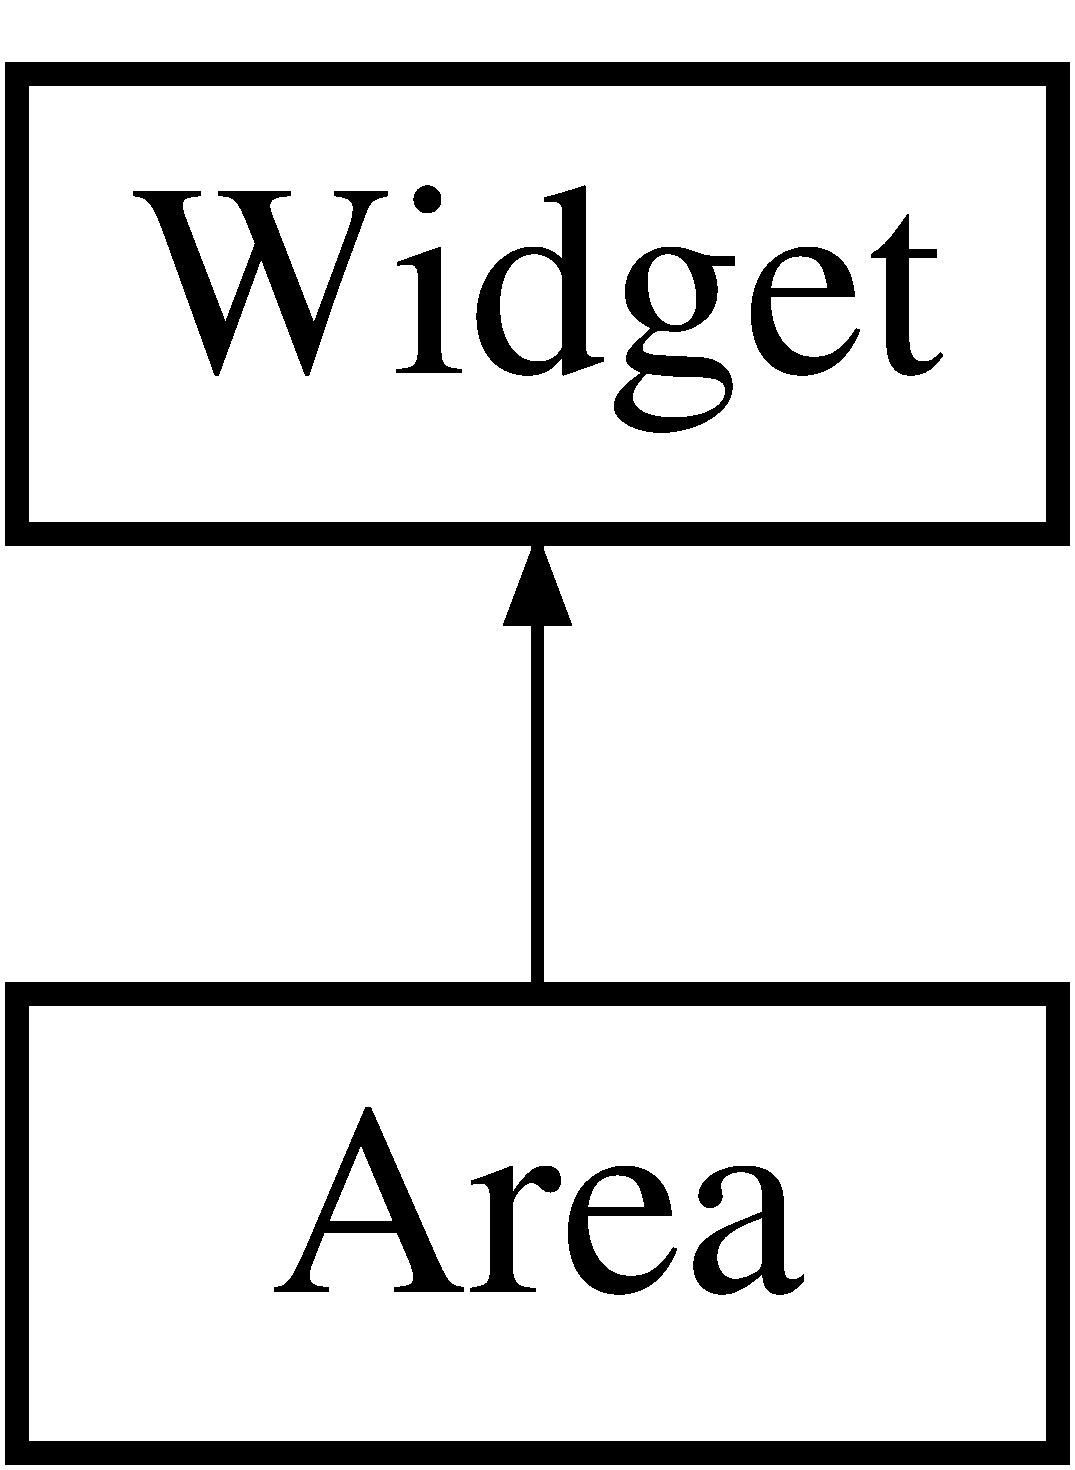
\includegraphics[height=2.000000cm]{class_area}
\end{center}
\end{figure}
\subsection*{Publikus tagfüggvények}
\begin{DoxyCompactItemize}
\item 
\hyperlink{class_area_a17542a72fc2a09713d5e9c90c2a99028}{Area} (int x, int y)
\begin{DoxyCompactList}\small\item\em L�trehoz egy �j ter�letet a X vagy O kijelz�s�re. \end{DoxyCompactList}\item 
void \hyperlink{class_area_aedf392939473fbf8e886b3878e411aea}{Set\+Event\+Void} (std\+::function$<$ void(\hyperlink{class_area}{Area} $\ast$)$>$ \hyperlink{structgenv_1_1event}{event})
\begin{DoxyCompactList}\small\item\em Be�ll�tja az esem�nyt, ami akkor k�vetkezik be, ha r�kattintanak. \end{DoxyCompactList}\item 
void \hyperlink{class_area_a78a2896834ec29e35c1289b7c73e3a98}{Set\+Value} (int value)
\begin{DoxyCompactList}\small\item\em Be�ll�tja az �rt�k�t \end{DoxyCompactList}\item 
void \hyperlink{class_area_a9420b052e63aee231e969aec168dbc03}{Set\+Marker\+Colour} (int r, int g, int b)
\begin{DoxyCompactList}\small\item\em A kijelz�s sz�n�t adja meg. \end{DoxyCompactList}\item 
int \hyperlink{class_area_aef3bb5bafb65da4ad27b570ec6327be4}{Get\+Value} ()
\begin{DoxyCompactList}\small\item\em Megadja az aktu�lis �rt�k�t \end{DoxyCompactList}\item 
int \hyperlink{class_area_a0e49be1c58b893fe6ad8c68b7ab5c3cb}{Get\+X\+Postion} ()
\begin{DoxyCompactList}\small\item\em Megadja az x koordin�t�j�t \end{DoxyCompactList}\item 
int \hyperlink{class_area_a328de42ab1d176e091726f2b459a45be}{Get\+Y\+Position} ()
\begin{DoxyCompactList}\small\item\em Megadja az y koordin�t�j�t \end{DoxyCompactList}\item 
virtual void \hyperlink{class_area_ac90399336ed7754946e274e443ed98ff}{Draw} ()
\begin{DoxyCompactList}\small\item\em Kirajzolja a widgetet. \end{DoxyCompactList}\item 
virtual void \hyperlink{class_area_a8917c7e4715659ae5021d2c9e40127f4}{Handle} (\hyperlink{structgenv_1_1event}{genv\+::event} ev)
\begin{DoxyCompactList}\small\item\em Kezeli a widgetet az inputnak megfelel�en. \end{DoxyCompactList}\item 
virtual bool \hyperlink{class_area_a9d309a54dbc62cd8edd8bc976644090c}{Is\+In\+Line} (int x, int y)
\begin{DoxyCompactList}\small\item\em Megadja, hogy egy koordin�ta rajta van-\/e a widgeten. \end{DoxyCompactList}\end{DoxyCompactItemize}
\subsection*{Privát attribútumok}
\begin{DoxyCompactItemize}
\item 
int \hyperlink{class_area_a7531aac606a8d9fa3ef3e70b28a7375e}{X\+Val}
\item 
int \hyperlink{class_area_a791b0f1915a30e990dca964afaaaecc2}{Y\+Val}
\item 
int \hyperlink{class_area_a3896accc992855520cb2eabc64ed09d0}{Value}
\item 
\hyperlink{class_colour}{Colour} $\ast$ \hyperlink{class_area_a5af595519a7061b9053de4a01bc072f6}{Mark\+Colour}
\item 
std\+::function$<$ void(\hyperlink{class_area}{Area} $\ast$)$>$ \hyperlink{class_area_a82637253c6ea81b16b0e26db9e9f87a8}{On\+Event}
\end{DoxyCompactItemize}
\subsection*{Additional Inherited Members}


\subsection{Konstruktorok és destruktorok dokumentációja}
\mbox{\Hypertarget{class_area_a17542a72fc2a09713d5e9c90c2a99028}\label{class_area_a17542a72fc2a09713d5e9c90c2a99028}} 
\index{Area@{Area}!Area@{Area}}
\index{Area@{Area}!Area@{Area}}
\subsubsection{\texorpdfstring{Area()}{Area()}}
{\footnotesize\ttfamily Area\+::\+Area (\begin{DoxyParamCaption}\item[{int}]{x,  }\item[{int}]{y }\end{DoxyParamCaption})}



L�trehoz egy �j ter�letet a X vagy O kijelz�s�re. 


\begin{DoxyParams}{Paraméterek}
{\em x} & int Az x koordin�ta \\
\hline
{\em y} & int Az y koordin�ta \\
\hline
\end{DoxyParams}


\subsection{Tagfüggvények dokumentációja}
\mbox{\Hypertarget{class_area_ac90399336ed7754946e274e443ed98ff}\label{class_area_ac90399336ed7754946e274e443ed98ff}} 
\index{Area@{Area}!Draw@{Draw}}
\index{Draw@{Draw}!Area@{Area}}
\subsubsection{\texorpdfstring{Draw()}{Draw()}}
{\footnotesize\ttfamily void Area\+::\+Draw (\begin{DoxyParamCaption}{ }\end{DoxyParamCaption})\hspace{0.3cm}{\ttfamily [virtual]}}



Kirajzolja a widgetet. 

\begin{DoxyReturn}{Visszatérési érték}
virtual void 
\end{DoxyReturn}


Megvalósítja a következőket\+: \hyperlink{class_widget_ac4c2063cd671468ad05d84cfe963c032}{Widget}.

\mbox{\Hypertarget{class_area_aef3bb5bafb65da4ad27b570ec6327be4}\label{class_area_aef3bb5bafb65da4ad27b570ec6327be4}} 
\index{Area@{Area}!Get\+Value@{Get\+Value}}
\index{Get\+Value@{Get\+Value}!Area@{Area}}
\subsubsection{\texorpdfstring{Get\+Value()}{GetValue()}}
{\footnotesize\ttfamily int Area\+::\+Get\+Value (\begin{DoxyParamCaption}{ }\end{DoxyParamCaption})}



Megadja az aktu�lis �rt�k�t 

\begin{DoxyReturn}{Visszatérési érték}
int Az aktu�lis �rt�k 
\end{DoxyReturn}
\mbox{\Hypertarget{class_area_a0e49be1c58b893fe6ad8c68b7ab5c3cb}\label{class_area_a0e49be1c58b893fe6ad8c68b7ab5c3cb}} 
\index{Area@{Area}!Get\+X\+Postion@{Get\+X\+Postion}}
\index{Get\+X\+Postion@{Get\+X\+Postion}!Area@{Area}}
\subsubsection{\texorpdfstring{Get\+X\+Postion()}{GetXPostion()}}
{\footnotesize\ttfamily int Area\+::\+Get\+X\+Postion (\begin{DoxyParamCaption}{ }\end{DoxyParamCaption})}



Megadja az x koordin�t�j�t 

\begin{DoxyReturn}{Visszatérési érték}
int Az x koordin�ta 
\end{DoxyReturn}
\mbox{\Hypertarget{class_area_a328de42ab1d176e091726f2b459a45be}\label{class_area_a328de42ab1d176e091726f2b459a45be}} 
\index{Area@{Area}!Get\+Y\+Position@{Get\+Y\+Position}}
\index{Get\+Y\+Position@{Get\+Y\+Position}!Area@{Area}}
\subsubsection{\texorpdfstring{Get\+Y\+Position()}{GetYPosition()}}
{\footnotesize\ttfamily int Area\+::\+Get\+Y\+Position (\begin{DoxyParamCaption}{ }\end{DoxyParamCaption})}



Megadja az y koordin�t�j�t 

\begin{DoxyReturn}{Visszatérési érték}
int Az y koordin�ta 
\end{DoxyReturn}
\mbox{\Hypertarget{class_area_a8917c7e4715659ae5021d2c9e40127f4}\label{class_area_a8917c7e4715659ae5021d2c9e40127f4}} 
\index{Area@{Area}!Handle@{Handle}}
\index{Handle@{Handle}!Area@{Area}}
\subsubsection{\texorpdfstring{Handle()}{Handle()}}
{\footnotesize\ttfamily void Area\+::\+Handle (\begin{DoxyParamCaption}\item[{\hyperlink{structgenv_1_1event}{genv\+::event}}]{ev }\end{DoxyParamCaption})\hspace{0.3cm}{\ttfamily [virtual]}}



Kezeli a widgetet az inputnak megfelel�en. 


\begin{DoxyParams}{Paraméterek}
{\em ev} & \hyperlink{structgenv_1_1event}{genv\+::event} Az input eventje \\
\hline
\end{DoxyParams}
\begin{DoxyReturn}{Visszatérési érték}
virtual void 
\end{DoxyReturn}


Megvalósítja a következőket\+: \hyperlink{class_widget_abf512e4606c7a5d44245a9b0246634a0}{Widget}.

\mbox{\Hypertarget{class_area_a9d309a54dbc62cd8edd8bc976644090c}\label{class_area_a9d309a54dbc62cd8edd8bc976644090c}} 
\index{Area@{Area}!Is\+In\+Line@{Is\+In\+Line}}
\index{Is\+In\+Line@{Is\+In\+Line}!Area@{Area}}
\subsubsection{\texorpdfstring{Is\+In\+Line()}{IsInLine()}}
{\footnotesize\ttfamily bool Area\+::\+Is\+In\+Line (\begin{DoxyParamCaption}\item[{int}]{x,  }\item[{int}]{y }\end{DoxyParamCaption})\hspace{0.3cm}{\ttfamily [virtual]}}



Megadja, hogy egy koordin�ta rajta van-\/e a widgeten. 


\begin{DoxyParams}{Paraméterek}
{\em x} & int Az x koordin�ta \\
\hline
{\em y} & int Az y koordin�ta \\
\hline
\end{DoxyParams}
\begin{DoxyReturn}{Visszatérési érték}
virtual bool 
\end{DoxyReturn}


Megvalósítja a következőket\+: \hyperlink{class_widget_a7a18323ef481add82e5edba5c0c6ec06}{Widget}.

\mbox{\Hypertarget{class_area_aedf392939473fbf8e886b3878e411aea}\label{class_area_aedf392939473fbf8e886b3878e411aea}} 
\index{Area@{Area}!Set\+Event\+Void@{Set\+Event\+Void}}
\index{Set\+Event\+Void@{Set\+Event\+Void}!Area@{Area}}
\subsubsection{\texorpdfstring{Set\+Event\+Void()}{SetEventVoid()}}
{\footnotesize\ttfamily void Area\+::\+Set\+Event\+Void (\begin{DoxyParamCaption}\item[{std\+::function$<$ void(\hyperlink{class_area}{Area} $\ast$)$>$}]{event }\end{DoxyParamCaption})}



Be�ll�tja az esem�nyt, ami akkor k�vetkezik be, ha r�kattintanak. 


\begin{DoxyParams}{Paraméterek}
{\em Area$\ast$} & Saj�t mag�t adja vissza \\
\hline
\end{DoxyParams}
\begin{DoxyReturn}{Visszatérési érték}
void 
\end{DoxyReturn}
\mbox{\Hypertarget{class_area_a9420b052e63aee231e969aec168dbc03}\label{class_area_a9420b052e63aee231e969aec168dbc03}} 
\index{Area@{Area}!Set\+Marker\+Colour@{Set\+Marker\+Colour}}
\index{Set\+Marker\+Colour@{Set\+Marker\+Colour}!Area@{Area}}
\subsubsection{\texorpdfstring{Set\+Marker\+Colour()}{SetMarkerColour()}}
{\footnotesize\ttfamily void Area\+::\+Set\+Marker\+Colour (\begin{DoxyParamCaption}\item[{int}]{r,  }\item[{int}]{g,  }\item[{int}]{b }\end{DoxyParamCaption})}



A kijelz�s sz�n�t adja meg. 


\begin{DoxyParams}{Paraméterek}
{\em r} & int A piros �rt�k \\
\hline
{\em g} & int A z�ld �rt�k \\
\hline
{\em b} & int A k�k �rt�k \\
\hline
\end{DoxyParams}
\begin{DoxyReturn}{Visszatérési érték}
void 
\end{DoxyReturn}
\mbox{\Hypertarget{class_area_a78a2896834ec29e35c1289b7c73e3a98}\label{class_area_a78a2896834ec29e35c1289b7c73e3a98}} 
\index{Area@{Area}!Set\+Value@{Set\+Value}}
\index{Set\+Value@{Set\+Value}!Area@{Area}}
\subsubsection{\texorpdfstring{Set\+Value()}{SetValue()}}
{\footnotesize\ttfamily void Area\+::\+Set\+Value (\begin{DoxyParamCaption}\item[{int}]{value }\end{DoxyParamCaption})}



Be�ll�tja az �rt�k�t 


\begin{DoxyParams}{Paraméterek}
{\em value} & int A be�ll�tand� �rt�k \\
\hline
\end{DoxyParams}
\begin{DoxyReturn}{Visszatérési érték}
void 
\end{DoxyReturn}


\subsection{Adattagok dokumentációja}
\mbox{\Hypertarget{class_area_a5af595519a7061b9053de4a01bc072f6}\label{class_area_a5af595519a7061b9053de4a01bc072f6}} 
\index{Area@{Area}!Mark\+Colour@{Mark\+Colour}}
\index{Mark\+Colour@{Mark\+Colour}!Area@{Area}}
\subsubsection{\texorpdfstring{Mark\+Colour}{MarkColour}}
{\footnotesize\ttfamily \hyperlink{class_colour}{Colour}$\ast$ Area\+::\+Mark\+Colour\hspace{0.3cm}{\ttfamily [private]}}

A kijelz�s sz�ne \mbox{\Hypertarget{class_area_a82637253c6ea81b16b0e26db9e9f87a8}\label{class_area_a82637253c6ea81b16b0e26db9e9f87a8}} 
\index{Area@{Area}!On\+Event@{On\+Event}}
\index{On\+Event@{On\+Event}!Area@{Area}}
\subsubsection{\texorpdfstring{On\+Event}{OnEvent}}
{\footnotesize\ttfamily std\+::function$<$void(\hyperlink{class_area}{Area}$\ast$)$>$ Area\+::\+On\+Event\hspace{0.3cm}{\ttfamily [private]}}

Az event hat�s�ra megh�v�d� esem�ny \mbox{\Hypertarget{class_area_a3896accc992855520cb2eabc64ed09d0}\label{class_area_a3896accc992855520cb2eabc64ed09d0}} 
\index{Area@{Area}!Value@{Value}}
\index{Value@{Value}!Area@{Area}}
\subsubsection{\texorpdfstring{Value}{Value}}
{\footnotesize\ttfamily int Area\+::\+Value\hspace{0.3cm}{\ttfamily [private]}}

Az aktu�lis �rt�ke \mbox{\Hypertarget{class_area_a7531aac606a8d9fa3ef3e70b28a7375e}\label{class_area_a7531aac606a8d9fa3ef3e70b28a7375e}} 
\index{Area@{Area}!X\+Val@{X\+Val}}
\index{X\+Val@{X\+Val}!Area@{Area}}
\subsubsection{\texorpdfstring{X\+Val}{XVal}}
{\footnotesize\ttfamily int Area\+::\+X\+Val\hspace{0.3cm}{\ttfamily [private]}}

Az x koordin�ta \mbox{\Hypertarget{class_area_a791b0f1915a30e990dca964afaaaecc2}\label{class_area_a791b0f1915a30e990dca964afaaaecc2}} 
\index{Area@{Area}!Y\+Val@{Y\+Val}}
\index{Y\+Val@{Y\+Val}!Area@{Area}}
\subsubsection{\texorpdfstring{Y\+Val}{YVal}}
{\footnotesize\ttfamily int Area\+::\+Y\+Val\hspace{0.3cm}{\ttfamily [private]}}

Az y koordin�ta 

Ez a dokumentáció az osztályról a következő fájlok alapján készült\+:\begin{DoxyCompactItemize}
\item 
Area.\+h\item 
Area.\+cpp\end{DoxyCompactItemize}

\hypertarget{classasd}{}\section{asd osztályreferencia}
\label{classasd}\index{asd@{asd}}


Ez a dokumentáció az osztályról a következő fájlok alapján készült\+:\begin{DoxyCompactItemize}
\item 
asd.\+h\item 
asd.\+cpp\end{DoxyCompactItemize}

\hypertarget{structgenv_1_1box}{}\section{genv\+:\+:box struktúrareferencia}
\label{structgenv_1_1box}\index{genv\+::box@{genv\+::box}}
\subsection*{Publikus tagfüggvények}
\begin{DoxyCompactItemize}
\item 
\mbox{\Hypertarget{structgenv_1_1box_af3503beee95ae0b5fa4a33fcdd75a0b5}\label{structgenv_1_1box_af3503beee95ae0b5fa4a33fcdd75a0b5}} 
{\bfseries box} (int x, int y)
\item 
\mbox{\Hypertarget{structgenv_1_1box_aa370a72cc0844a0dcb18efd335dc2c72}\label{structgenv_1_1box_aa370a72cc0844a0dcb18efd335dc2c72}} 
void {\bfseries operator()} (\hyperlink{classgenv_1_1canvas}{canvas} \&out)
\end{DoxyCompactItemize}
\subsection*{Publikus attribútumok}
\begin{DoxyCompactItemize}
\item 
\mbox{\Hypertarget{structgenv_1_1box_af28b87b7187c6d544168b96201ea31f6}\label{structgenv_1_1box_af28b87b7187c6d544168b96201ea31f6}} 
int {\bfseries vec\+\_\+x}
\item 
\mbox{\Hypertarget{structgenv_1_1box_a7d0c1be9618a7b76b3b411d0501275cb}\label{structgenv_1_1box_a7d0c1be9618a7b76b3b411d0501275cb}} 
int {\bfseries vec\+\_\+y}
\end{DoxyCompactItemize}


Ez a dokumentáció a struktúráról a következő fájl alapján készült\+:\begin{DoxyCompactItemize}
\item 
graphics.\+hpp\end{DoxyCompactItemize}

\hypertarget{structgenv_1_1box__to}{}\section{genv\+:\+:box\+\_\+to struktúrareferencia}
\label{structgenv_1_1box__to}\index{genv\+::box\+\_\+to@{genv\+::box\+\_\+to}}
\subsection*{Publikus tagfüggvények}
\begin{DoxyCompactItemize}
\item 
\mbox{\Hypertarget{structgenv_1_1box__to_a0d5524a0b4d159d3fc6b89a9c13d4bdf}\label{structgenv_1_1box__to_a0d5524a0b4d159d3fc6b89a9c13d4bdf}} 
{\bfseries box\+\_\+to} (unsigned x, unsigned y)
\item 
\mbox{\Hypertarget{structgenv_1_1box__to_a7f1d42b300184be6c383bea7fabfc74b}\label{structgenv_1_1box__to_a7f1d42b300184be6c383bea7fabfc74b}} 
void {\bfseries operator()} (\hyperlink{classgenv_1_1canvas}{canvas} \&out)
\end{DoxyCompactItemize}
\subsection*{Publikus attribútumok}
\begin{DoxyCompactItemize}
\item 
\mbox{\Hypertarget{structgenv_1_1box__to_a137dbe74c0bc47a4ce80558649017be2}\label{structgenv_1_1box__to_a137dbe74c0bc47a4ce80558649017be2}} 
int {\bfseries pos\+\_\+x}
\item 
\mbox{\Hypertarget{structgenv_1_1box__to_ae29e53f61817b3ffbc1a6cd63b45e332}\label{structgenv_1_1box__to_ae29e53f61817b3ffbc1a6cd63b45e332}} 
int {\bfseries pos\+\_\+y}
\end{DoxyCompactItemize}


Ez a dokumentáció a struktúráról a következő fájl alapján készült\+:\begin{DoxyCompactItemize}
\item 
graphics.\+hpp\end{DoxyCompactItemize}

\hypertarget{class_button}{}\section{Button osztályreferencia}
\label{class_button}\index{Button@{Button}}
A Button osztály származási diagramja\+:\begin{figure}[H]
\begin{center}
\leavevmode
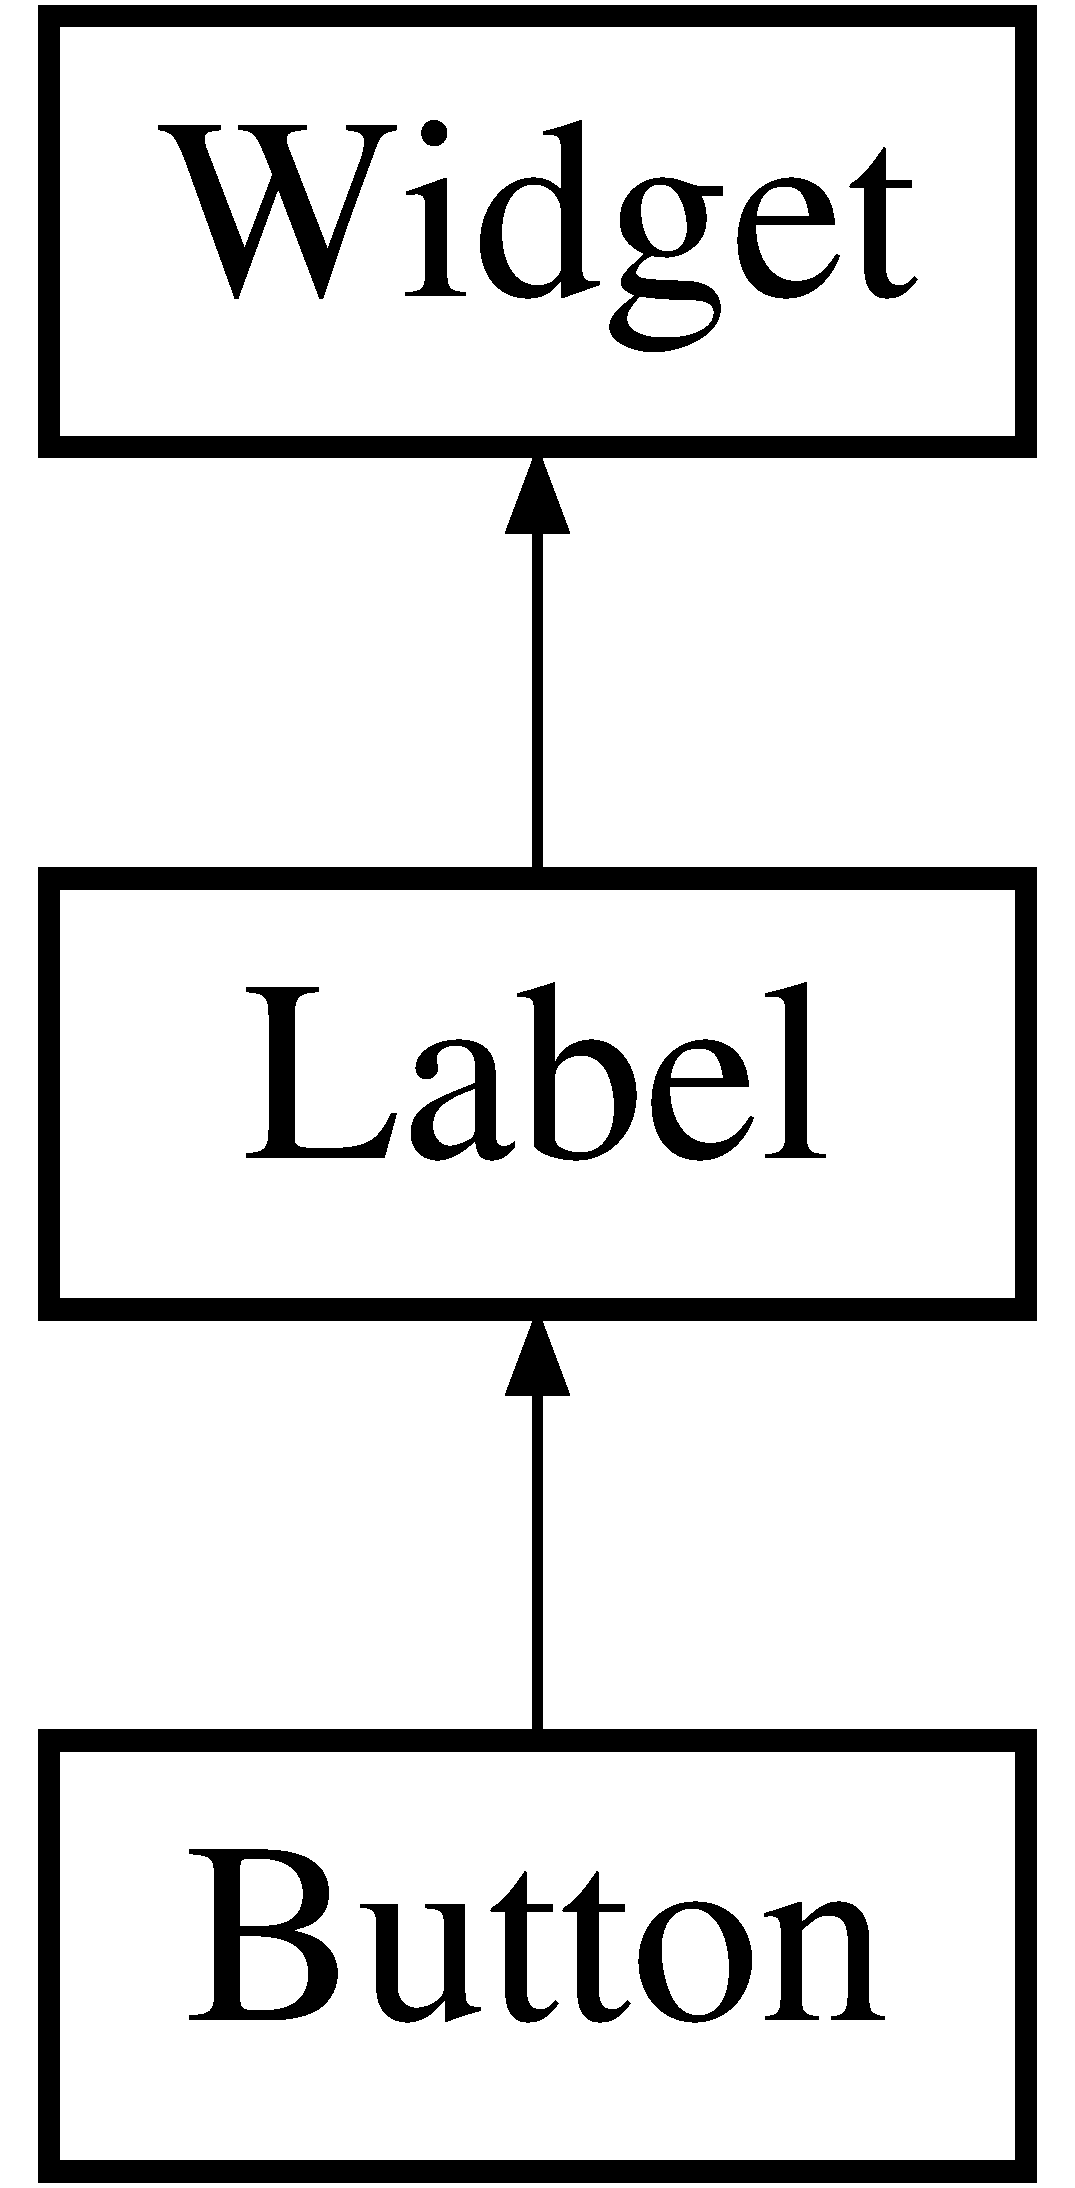
\includegraphics[height=3.000000cm]{class_button}
\end{center}
\end{figure}
\subsection*{Publikus tagfüggvények}
\begin{DoxyCompactItemize}
\item 
\hyperlink{class_button_a33553572657626500239c144f1bbc04f}{Button} (int x, int y, int x\+Size, int y\+Size, std\+::string text, std\+::function$<$ void()$>$ fv)
\begin{DoxyCompactList}\small\item\em Létrehoz egy új gombot. \end{DoxyCompactList}\item 
virtual void \hyperlink{class_button_a6aaa2b781c933a296f41a8eca890eb1f}{Draw} ()
\begin{DoxyCompactList}\small\item\em Kirajzolja a widgetet. \end{DoxyCompactList}\item 
virtual void \hyperlink{class_button_a72dc68b7a78edfebe904bf489d6e03fb}{Handle} (\hyperlink{structgenv_1_1event}{genv\+::event} ev)
\begin{DoxyCompactList}\small\item\em Kezeli a widgetet az inputnak megfelelõen. \end{DoxyCompactList}\item 
virtual bool \hyperlink{class_button_a61832186fb0cf58c4c1c6fbbe572b61c}{Is\+In\+Line} (int x, int y)
\begin{DoxyCompactList}\small\item\em Megadja, hogy egy koordináta rajta van-\/e a widgeten. \end{DoxyCompactList}\item 
void \hyperlink{class_button_aa9bb1fc7a079ef575f255f9c7e4fcfbb}{Set\+On\+Click\+Color} (int r, int g, int b)
\begin{DoxyCompactList}\small\item\em A kattintáskor látható színt változtatja meg. \end{DoxyCompactList}\end{DoxyCompactItemize}
\subsection*{Privát attribútumok}
\begin{DoxyCompactItemize}
\item 
std\+::function$<$ void()$>$ \hyperlink{class_button_ac125da6324c6d2e107eea9072a6eb351}{Function}
\item 
\hyperlink{class_colour}{Colour} $\ast$ \hyperlink{class_button_a16b3b12b5112e4e9fe88e8f84f4a6dcc}{On\+Click\+Color}
\item 
bool \hyperlink{class_button_a166458b3e6dc6161b64f65a30a8cb31c}{is\+Clicking}
\end{DoxyCompactItemize}
\subsection*{Additional Inherited Members}


\subsection{Konstruktorok és destruktorok dokumentációja}
\mbox{\Hypertarget{class_button_a33553572657626500239c144f1bbc04f}\label{class_button_a33553572657626500239c144f1bbc04f}} 
\index{Button@{Button}!Button@{Button}}
\index{Button@{Button}!Button@{Button}}
\subsubsection{\texorpdfstring{Button()}{Button()}}
{\footnotesize\ttfamily Button\+::\+Button (\begin{DoxyParamCaption}\item[{int}]{x,  }\item[{int}]{y,  }\item[{int}]{x\+Size,  }\item[{int}]{y\+Size,  }\item[{std\+::string}]{text,  }\item[{std\+::function$<$ void()$>$}]{fv }\end{DoxyParamCaption})}



Létrehoz egy új gombot. 

\begin{DoxyReturn}{Visszatérési érték}
\hyperlink{class_button}{Button}(int x, int y, int x\+Size, int y\+Size, std\+::string text, 
\end{DoxyReturn}


\subsection{Tagfüggvények dokumentációja}
\mbox{\Hypertarget{class_button_a6aaa2b781c933a296f41a8eca890eb1f}\label{class_button_a6aaa2b781c933a296f41a8eca890eb1f}} 
\index{Button@{Button}!Draw@{Draw}}
\index{Draw@{Draw}!Button@{Button}}
\subsubsection{\texorpdfstring{Draw()}{Draw()}}
{\footnotesize\ttfamily void Button\+::\+Draw (\begin{DoxyParamCaption}{ }\end{DoxyParamCaption})\hspace{0.3cm}{\ttfamily [virtual]}}



Kirajzolja a widgetet. 

\begin{DoxyReturn}{Visszatérési érték}
virtual void 
\end{DoxyReturn}


Újraimplementált ősök\+: \hyperlink{class_label_a184df028b3aa8c7f8dec8ecb90533319}{Label}.

\mbox{\Hypertarget{class_button_a72dc68b7a78edfebe904bf489d6e03fb}\label{class_button_a72dc68b7a78edfebe904bf489d6e03fb}} 
\index{Button@{Button}!Handle@{Handle}}
\index{Handle@{Handle}!Button@{Button}}
\subsubsection{\texorpdfstring{Handle()}{Handle()}}
{\footnotesize\ttfamily void Button\+::\+Handle (\begin{DoxyParamCaption}\item[{\hyperlink{structgenv_1_1event}{genv\+::event}}]{ev }\end{DoxyParamCaption})\hspace{0.3cm}{\ttfamily [virtual]}}



Kezeli a widgetet az inputnak megfelelõen. 


\begin{DoxyParams}{Paraméterek}
{\em ev} & \hyperlink{structgenv_1_1event}{genv\+::event} Az input eventje \\
\hline
\end{DoxyParams}
\begin{DoxyReturn}{Visszatérési érték}
virtual void 
\end{DoxyReturn}


Újraimplementált ősök\+: \hyperlink{class_label_a5cf04da7def075453b5c0fda93a1b575}{Label}.

\mbox{\Hypertarget{class_button_a61832186fb0cf58c4c1c6fbbe572b61c}\label{class_button_a61832186fb0cf58c4c1c6fbbe572b61c}} 
\index{Button@{Button}!Is\+In\+Line@{Is\+In\+Line}}
\index{Is\+In\+Line@{Is\+In\+Line}!Button@{Button}}
\subsubsection{\texorpdfstring{Is\+In\+Line()}{IsInLine()}}
{\footnotesize\ttfamily bool Button\+::\+Is\+In\+Line (\begin{DoxyParamCaption}\item[{int}]{x,  }\item[{int}]{y }\end{DoxyParamCaption})\hspace{0.3cm}{\ttfamily [virtual]}}



Megadja, hogy egy koordináta rajta van-\/e a widgeten. 


\begin{DoxyParams}{Paraméterek}
{\em x} & int Az x koordináta \\
\hline
{\em y} & int Az y koordináta \\
\hline
\end{DoxyParams}
\begin{DoxyReturn}{Visszatérési érték}
virtual bool 
\end{DoxyReturn}


Újraimplementált ősök\+: \hyperlink{class_label_a918ebb45dbaa5484643355cf5ab4be47}{Label}.

\mbox{\Hypertarget{class_button_aa9bb1fc7a079ef575f255f9c7e4fcfbb}\label{class_button_aa9bb1fc7a079ef575f255f9c7e4fcfbb}} 
\index{Button@{Button}!Set\+On\+Click\+Color@{Set\+On\+Click\+Color}}
\index{Set\+On\+Click\+Color@{Set\+On\+Click\+Color}!Button@{Button}}
\subsubsection{\texorpdfstring{Set\+On\+Click\+Color()}{SetOnClickColor()}}
{\footnotesize\ttfamily void Button\+::\+Set\+On\+Click\+Color (\begin{DoxyParamCaption}\item[{int}]{r,  }\item[{int}]{g,  }\item[{int}]{b }\end{DoxyParamCaption})}



A kattintáskor látható színt változtatja meg. 


\begin{DoxyParams}{Paraméterek}
{\em r} & int Az új szín piros értéke \\
\hline
{\em g} & int Az új szín zöld értéke \\
\hline
{\em b} & int Az új szín kék értéke \\
\hline
\end{DoxyParams}
\begin{DoxyReturn}{Visszatérési érték}
void 
\end{DoxyReturn}


\subsection{Adattagok dokumentációja}
\mbox{\Hypertarget{class_button_ac125da6324c6d2e107eea9072a6eb351}\label{class_button_ac125da6324c6d2e107eea9072a6eb351}} 
\index{Button@{Button}!Function@{Function}}
\index{Function@{Function}!Button@{Button}}
\subsubsection{\texorpdfstring{Function}{Function}}
{\footnotesize\ttfamily std\+::function$<$void()$>$ Button\+::\+Function\hspace{0.3cm}{\ttfamily [private]}}

A kattintáskor meghívandó funció \mbox{\Hypertarget{class_button_a166458b3e6dc6161b64f65a30a8cb31c}\label{class_button_a166458b3e6dc6161b64f65a30a8cb31c}} 
\index{Button@{Button}!is\+Clicking@{is\+Clicking}}
\index{is\+Clicking@{is\+Clicking}!Button@{Button}}
\subsubsection{\texorpdfstring{is\+Clicking}{isClicking}}
{\footnotesize\ttfamily bool Button\+::is\+Clicking\hspace{0.3cm}{\ttfamily [private]}}

Le van-\/e nyomva a gomb \mbox{\Hypertarget{class_button_a16b3b12b5112e4e9fe88e8f84f4a6dcc}\label{class_button_a16b3b12b5112e4e9fe88e8f84f4a6dcc}} 
\index{Button@{Button}!On\+Click\+Color@{On\+Click\+Color}}
\index{On\+Click\+Color@{On\+Click\+Color}!Button@{Button}}
\subsubsection{\texorpdfstring{On\+Click\+Color}{OnClickColor}}
{\footnotesize\ttfamily \hyperlink{class_colour}{Colour}$\ast$ Button\+::\+On\+Click\+Color\hspace{0.3cm}{\ttfamily [private]}}

A kattintáskor látható szín 

Ez a dokumentáció az osztályról a következő fájlok alapján készült\+:\begin{DoxyCompactItemize}
\item 
Button.\+h\item 
Button.\+cpp\end{DoxyCompactItemize}

\hypertarget{classgenv_1_1canvas}{}\section{genv\+:\+:canvas osztályreferencia}
\label{classgenv_1_1canvas}\index{genv\+::canvas@{genv\+::canvas}}
A genv\+:\+:canvas osztály származási diagramja\+:\begin{figure}[H]
\begin{center}
\leavevmode
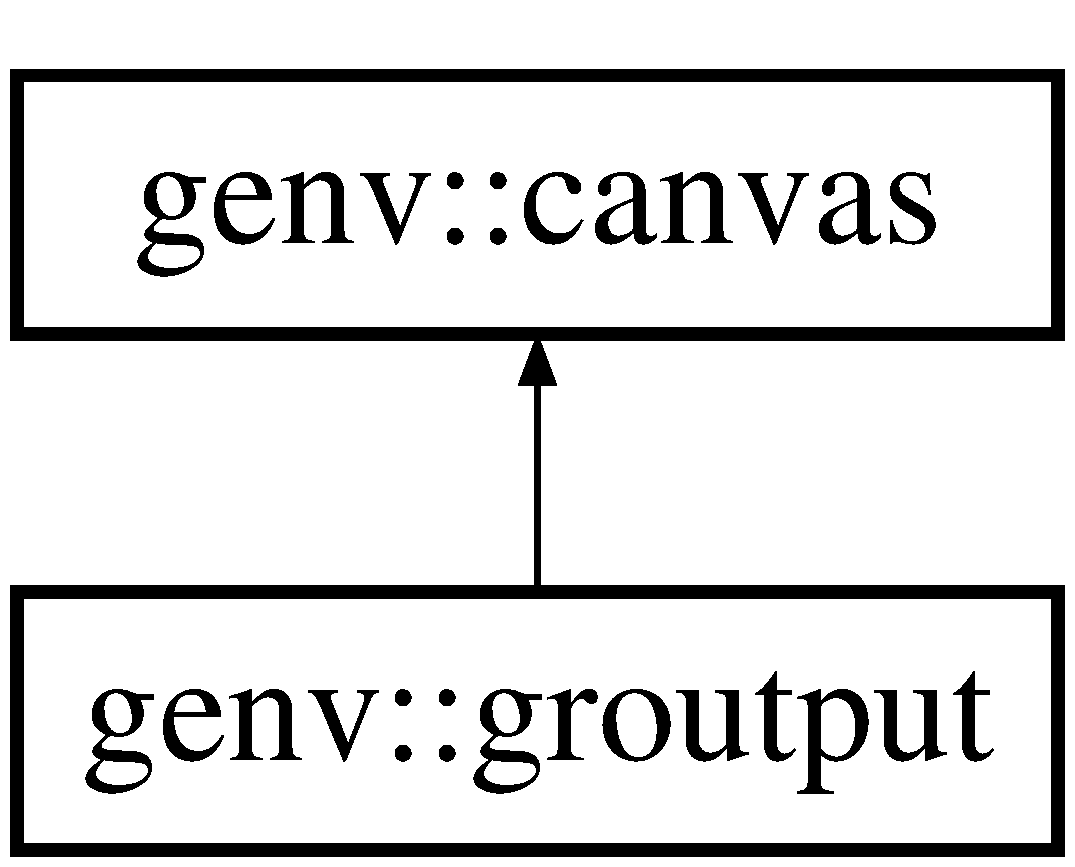
\includegraphics[height=2.000000cm]{classgenv_1_1canvas}
\end{center}
\end{figure}
\subsection*{Publikus tagfüggvények}
\begin{DoxyCompactItemize}
\item 
\mbox{\Hypertarget{classgenv_1_1canvas_ae4210ffb2450a3ba02df10dc54e51450}\label{classgenv_1_1canvas_ae4210ffb2450a3ba02df10dc54e51450}} 
{\bfseries canvas} (int w, int h)
\item 
\mbox{\Hypertarget{classgenv_1_1canvas_a86451ee2e5574e00d3afc56333f531e4}\label{classgenv_1_1canvas_a86451ee2e5574e00d3afc56333f531e4}} 
{\bfseries canvas} (const \hyperlink{classgenv_1_1canvas}{canvas} \&c)
\item 
\mbox{\Hypertarget{classgenv_1_1canvas_ab39f2907cf7fda9c27246e9e644877e8}\label{classgenv_1_1canvas_ab39f2907cf7fda9c27246e9e644877e8}} 
\hyperlink{classgenv_1_1canvas}{genv\+::canvas} \& {\bfseries operator=} (const \hyperlink{classgenv_1_1canvas}{genv\+::canvas} \&c)
\item 
\mbox{\Hypertarget{classgenv_1_1canvas_aeb1d899ae60e28a104923d3b63266638}\label{classgenv_1_1canvas_aeb1d899ae60e28a104923d3b63266638}} 
bool {\bfseries open} (unsigned width, unsigned height)
\item 
\mbox{\Hypertarget{classgenv_1_1canvas_a8f1a7098176b298409a1aeb9dfdb6333}\label{classgenv_1_1canvas_a8f1a7098176b298409a1aeb9dfdb6333}} 
bool {\bfseries save} (const std\+::string \&file) const
\item 
\mbox{\Hypertarget{classgenv_1_1canvas_a05e9e3bc7664435b02175325e667ffcc}\label{classgenv_1_1canvas_a05e9e3bc7664435b02175325e667ffcc}} 
void {\bfseries transparent} (bool t)
\item 
\mbox{\Hypertarget{classgenv_1_1canvas_a085f91bf2c74631935ba2fe7cc0a6002}\label{classgenv_1_1canvas_a085f91bf2c74631935ba2fe7cc0a6002}} 
void {\bfseries set\+\_\+color} (int r, int g, int b)
\item 
\mbox{\Hypertarget{classgenv_1_1canvas_a03b50301a46098ee2e0ba4e4203e3995}\label{classgenv_1_1canvas_a03b50301a46098ee2e0ba4e4203e3995}} 
bool {\bfseries move\+\_\+point} (int x, int y)
\item 
\mbox{\Hypertarget{classgenv_1_1canvas_a767d2a082da511ab6e84d4d7b98360be}\label{classgenv_1_1canvas_a767d2a082da511ab6e84d4d7b98360be}} 
void {\bfseries draw\+\_\+dot} ()
\item 
\mbox{\Hypertarget{classgenv_1_1canvas_a89a4e72f7064389cbe9418646863e919}\label{classgenv_1_1canvas_a89a4e72f7064389cbe9418646863e919}} 
void {\bfseries draw\+\_\+line} (int x, int y)
\item 
\mbox{\Hypertarget{classgenv_1_1canvas_aea31b05cd41534691b329bd1545eeb84}\label{classgenv_1_1canvas_aea31b05cd41534691b329bd1545eeb84}} 
void {\bfseries draw\+\_\+box} (int x, int y)
\item 
\mbox{\Hypertarget{classgenv_1_1canvas_a6c6b77a47bde4163919ad44dfa6e0638}\label{classgenv_1_1canvas_a6c6b77a47bde4163919ad44dfa6e0638}} 
void {\bfseries draw\+\_\+text} (const std\+::string \&str)
\item 
\mbox{\Hypertarget{classgenv_1_1canvas_a94bad016a557ab62c7019ca25647bc0c}\label{classgenv_1_1canvas_a94bad016a557ab62c7019ca25647bc0c}} 
void {\bfseries blitfrom} (const \hyperlink{classgenv_1_1canvas}{canvas} \&c, short x1, short y1, unsigned short x2, unsigned short y2, short x3, short y3)
\item 
\mbox{\Hypertarget{classgenv_1_1canvas_a8ecb2e0d7f15f8a4875e04f747762a13}\label{classgenv_1_1canvas_a8ecb2e0d7f15f8a4875e04f747762a13}} 
bool {\bfseries load\+\_\+font} (const std\+::string \&fname, int fontsize=16, bool antialias=true)
\item 
\mbox{\Hypertarget{classgenv_1_1canvas_ad57cbfa2d960d827e5f689c508255254}\label{classgenv_1_1canvas_ad57cbfa2d960d827e5f689c508255254}} 
void {\bfseries set\+\_\+antialias} (bool antialias)
\item 
\mbox{\Hypertarget{classgenv_1_1canvas_ad220ddfad4b67f2e24e2699e2ad7f91e}\label{classgenv_1_1canvas_ad220ddfad4b67f2e24e2699e2ad7f91e}} 
int {\bfseries x} () const
\item 
\mbox{\Hypertarget{classgenv_1_1canvas_a56c80674a756a69f09c0ce63bf17402d}\label{classgenv_1_1canvas_a56c80674a756a69f09c0ce63bf17402d}} 
int {\bfseries y} () const
\item 
\mbox{\Hypertarget{classgenv_1_1canvas_a21c0c57177ee0e47eb444a6bae8b7da5}\label{classgenv_1_1canvas_a21c0c57177ee0e47eb444a6bae8b7da5}} 
int {\bfseries cascent} () const
\item 
\mbox{\Hypertarget{classgenv_1_1canvas_ae90f845816ac7045be771cca107f6f73}\label{classgenv_1_1canvas_ae90f845816ac7045be771cca107f6f73}} 
int {\bfseries cdescent} () const
\item 
\mbox{\Hypertarget{classgenv_1_1canvas_a79b09f2fa46b713164ddc326fb5c7c31}\label{classgenv_1_1canvas_a79b09f2fa46b713164ddc326fb5c7c31}} 
int {\bfseries twidth} (const std\+::string \&s) const
\item 
\mbox{\Hypertarget{classgenv_1_1canvas_a04bc3204672ade4baa0a13a10a43d9e2}\label{classgenv_1_1canvas_a04bc3204672ade4baa0a13a10a43d9e2}} 
virtual void {\bfseries refresh} ()
\item 
\mbox{\Hypertarget{classgenv_1_1canvas_a6a4a48ca686c16460d0c42e9d8c2ea3c}\label{classgenv_1_1canvas_a6a4a48ca686c16460d0c42e9d8c2ea3c}} 
{\footnotesize template$<$typename T $>$ }\\void {\bfseries call\+\_\+with\+\_\+rel} (T meth, int vec\+\_\+x, int vec\+\_\+y)
\end{DoxyCompactItemize}
\subsection*{Védett tagfüggvények}
\begin{DoxyCompactItemize}
\item 
\mbox{\Hypertarget{classgenv_1_1canvas_a7d2385f86f8e25db8c3a9254037e42df}\label{classgenv_1_1canvas_a7d2385f86f8e25db8c3a9254037e42df}} 
{\footnotesize template$<$typename T $>$ }\\int {\bfseries sgn} (const T \&a)
\end{DoxyCompactItemize}
\subsection*{Védett attribútumok}
\begin{DoxyCompactItemize}
\item 
\mbox{\Hypertarget{classgenv_1_1canvas_a4b7ebfdeae85fea93d7d42627e7a4919}\label{classgenv_1_1canvas_a4b7ebfdeae85fea93d7d42627e7a4919}} 
short {\bfseries pt\+\_\+x}
\item 
\mbox{\Hypertarget{classgenv_1_1canvas_ab6429e418598bad6fe741dbe91f5be6b}\label{classgenv_1_1canvas_ab6429e418598bad6fe741dbe91f5be6b}} 
short {\bfseries pt\+\_\+y}
\item 
\mbox{\Hypertarget{classgenv_1_1canvas_a6ca0cd219fcf31c40782584639d2529a}\label{classgenv_1_1canvas_a6ca0cd219fcf31c40782584639d2529a}} 
S\+D\+L\+\_\+\+Surface $\ast$ {\bfseries buf}
\item 
\mbox{\Hypertarget{classgenv_1_1canvas_a016e8269b583c1cee52b462ddcf12da9}\label{classgenv_1_1canvas_a016e8269b583c1cee52b462ddcf12da9}} 
int {\bfseries draw\+\_\+clr}
\item 
\mbox{\Hypertarget{classgenv_1_1canvas_a3c35d75d98e09c7a631cdba7ad80ed7e}\label{classgenv_1_1canvas_a3c35d75d98e09c7a631cdba7ad80ed7e}} 
bool {\bfseries transp}
\item 
\mbox{\Hypertarget{classgenv_1_1canvas_a2c732f76f91edcc63269a964a87d4e99}\label{classgenv_1_1canvas_a2c732f76f91edcc63269a964a87d4e99}} 
\+\_\+\+T\+T\+F\+\_\+\+Font $\ast$ {\bfseries font}
\item 
\mbox{\Hypertarget{classgenv_1_1canvas_a4def7539f99a07252d83a2ebe11c5116}\label{classgenv_1_1canvas_a4def7539f99a07252d83a2ebe11c5116}} 
bool {\bfseries antialiastext}
\item 
\mbox{\Hypertarget{classgenv_1_1canvas_a9d432f9f584dfe620becf4fe30ea5fb9}\label{classgenv_1_1canvas_a9d432f9f584dfe620becf4fe30ea5fb9}} 
std\+::string {\bfseries loaded\+\_\+font\+\_\+file\+\_\+name}
\item 
\mbox{\Hypertarget{classgenv_1_1canvas_a53d8e4a8b3d3d88330783b999be8e6ef}\label{classgenv_1_1canvas_a53d8e4a8b3d3d88330783b999be8e6ef}} 
int {\bfseries font\+\_\+size}
\end{DoxyCompactItemize}


Ez a dokumentáció az osztályról a következő fájl alapján készült\+:\begin{DoxyCompactItemize}
\item 
graphics.\+hpp\end{DoxyCompactItemize}

\hypertarget{structgenv_1_1color}{}\section{genv\+:\+:color struktúrareferencia}
\label{structgenv_1_1color}\index{genv\+::color@{genv\+::color}}
\subsection*{Publikus tagfüggvények}
\begin{DoxyCompactItemize}
\item 
\mbox{\Hypertarget{structgenv_1_1color_a212f9aeefe4fd3fd95dfca0cbfc286cd}\label{structgenv_1_1color_a212f9aeefe4fd3fd95dfca0cbfc286cd}} 
{\bfseries color} (int r, int g, int b)
\item 
\mbox{\Hypertarget{structgenv_1_1color_a88efd3188c6cffa85ba3422e7e32c0d9}\label{structgenv_1_1color_a88efd3188c6cffa85ba3422e7e32c0d9}} 
void {\bfseries operator()} (\hyperlink{classgenv_1_1canvas}{canvas} \&out)
\end{DoxyCompactItemize}
\subsection*{Publikus attribútumok}
\begin{DoxyCompactItemize}
\item 
\mbox{\Hypertarget{structgenv_1_1color_a0b861888917127b3c11c09130a8b02c3}\label{structgenv_1_1color_a0b861888917127b3c11c09130a8b02c3}} 
int {\bfseries red}
\item 
\mbox{\Hypertarget{structgenv_1_1color_ab7ba9f8dcf43ea8f3e0b644044d3dc52}\label{structgenv_1_1color_ab7ba9f8dcf43ea8f3e0b644044d3dc52}} 
int {\bfseries green}
\item 
\mbox{\Hypertarget{structgenv_1_1color_a02a4b955c8dec0e12ac18d9359cef52e}\label{structgenv_1_1color_a02a4b955c8dec0e12ac18d9359cef52e}} 
int {\bfseries blue}
\end{DoxyCompactItemize}


Ez a dokumentáció a struktúráról a következő fájl alapján készült\+:\begin{DoxyCompactItemize}
\item 
graphics.\+hpp\end{DoxyCompactItemize}

\hypertarget{class_colour}{}\section{Colour osztályreferencia}
\label{class_colour}\index{Colour@{Colour}}
\subsection*{Publikus tagfüggvények}
\begin{DoxyCompactItemize}
\item 
\hyperlink{class_colour_a46612b9524fcd4cee818af6a86b7a4d2}{Colour} ()
\item 
\hyperlink{class_colour_a88131e7210ca30c64fcf0d73d4705945}{Colour} (int r, int g, int b)
\item 
void \hyperlink{class_colour_a8781ecef0908fa0b0795e35a0282c4c9}{Adjust\+Colour} (int r, int g, int b)
\item 
void \hyperlink{class_colour_ada133c508a2b08f0884e260daee0bb82}{Set\+Colour} (int r, int g, int b)
\item 
void \hyperlink{class_colour_a403a38c1c711785622f8bacfadbb2801}{Set\+This\+Colour} ()
\item 
int \hyperlink{class_colour_aa520286f0c3e65e02298dafd98e730af}{GetR} ()
\item 
int \hyperlink{class_colour_a5867c71ecb081868729f81e9c2f104b1}{GetG} ()
\item 
int \hyperlink{class_colour_a1fbadc37dbe6ca5d7f9e40356a0b8213}{GetB} ()
\end{DoxyCompactItemize}
\subsection*{Privát tagfüggvények}
\begin{DoxyCompactItemize}
\item 
void \hyperlink{class_colour_a6b770134b677d05d9062fe55a5466e03}{Check\+R\+GB} ()
\end{DoxyCompactItemize}
\subsection*{Privát attribútumok}
\begin{DoxyCompactItemize}
\item 
int \hyperlink{class_colour_a2045bcd0534cd4cf0bd025571ac72feb}{R}
\item 
int \hyperlink{class_colour_a05957ae575ef990faf6f24ef1f6eb828}{G}
\item 
int \hyperlink{class_colour_a25ef99016bc619acb35d25e0eb86cad6}{B}
\end{DoxyCompactItemize}


\subsection{Konstruktorok és destruktorok dokumentációja}
\mbox{\Hypertarget{class_colour_a46612b9524fcd4cee818af6a86b7a4d2}\label{class_colour_a46612b9524fcd4cee818af6a86b7a4d2}} 
\index{Colour@{Colour}!Colour@{Colour}}
\index{Colour@{Colour}!Colour@{Colour}}
\subsubsection{\texorpdfstring{Colour()}{Colour()}\hspace{0.1cm}{\footnotesize\ttfamily [1/2]}}
{\footnotesize\ttfamily Colour\+::\+Colour (\begin{DoxyParamCaption}{ }\end{DoxyParamCaption})}

Egy sz�n R\+GB k�dj�t t�rolja, alap�rtelmezetten fekete \mbox{\Hypertarget{class_colour_a88131e7210ca30c64fcf0d73d4705945}\label{class_colour_a88131e7210ca30c64fcf0d73d4705945}} 
\index{Colour@{Colour}!Colour@{Colour}}
\index{Colour@{Colour}!Colour@{Colour}}
\subsubsection{\texorpdfstring{Colour()}{Colour()}\hspace{0.1cm}{\footnotesize\ttfamily [2/2]}}
{\footnotesize\ttfamily Colour\+::\+Colour (\begin{DoxyParamCaption}\item[{int}]{r,  }\item[{int}]{g,  }\item[{int}]{b }\end{DoxyParamCaption})}

Egy sz�n R\+GB k�dj�t t�rolja 
\begin{DoxyParams}{Paraméterek}
{\em r} & a sz�n piros k�dja \\
\hline
{\em g} & a sz�n z�ld k�dja \\
\hline
{\em b} & a sz�n k�k k�dja \\
\hline
\end{DoxyParams}


\subsection{Tagfüggvények dokumentációja}
\mbox{\Hypertarget{class_colour_a8781ecef0908fa0b0795e35a0282c4c9}\label{class_colour_a8781ecef0908fa0b0795e35a0282c4c9}} 
\index{Colour@{Colour}!Adjust\+Colour@{Adjust\+Colour}}
\index{Adjust\+Colour@{Adjust\+Colour}!Colour@{Colour}}
\subsubsection{\texorpdfstring{Adjust\+Colour()}{AdjustColour()}}
{\footnotesize\ttfamily void Colour\+::\+Adjust\+Colour (\begin{DoxyParamCaption}\item[{int}]{r,  }\item[{int}]{g,  }\item[{int}]{b }\end{DoxyParamCaption})}

A sz�nt m�dos�tja a megadott �rt�kekkel 
\begin{DoxyParams}{Paraméterek}
{\em r} & a piros m�dos�t�s m�rt�ke \\
\hline
{\em g} & a z�ld m�dos�t�s m�rt�ke \\
\hline
{\em b} & a k�k m�dos�t�s m�rt�ke \\
\hline
\end{DoxyParams}
\mbox{\Hypertarget{class_colour_a6b770134b677d05d9062fe55a5466e03}\label{class_colour_a6b770134b677d05d9062fe55a5466e03}} 
\index{Colour@{Colour}!Check\+R\+GB@{Check\+R\+GB}}
\index{Check\+R\+GB@{Check\+R\+GB}!Colour@{Colour}}
\subsubsection{\texorpdfstring{Check\+R\+G\+B()}{CheckRGB()}}
{\footnotesize\ttfamily void Colour\+::\+Check\+R\+GB (\begin{DoxyParamCaption}{ }\end{DoxyParamCaption})\hspace{0.3cm}{\ttfamily [private]}}

Ellen�rzi, hogy a sz�nek nem-\/e l�gnak ki a 0-\/255 tartom�nyb�l \mbox{\Hypertarget{class_colour_a1fbadc37dbe6ca5d7f9e40356a0b8213}\label{class_colour_a1fbadc37dbe6ca5d7f9e40356a0b8213}} 
\index{Colour@{Colour}!GetB@{GetB}}
\index{GetB@{GetB}!Colour@{Colour}}
\subsubsection{\texorpdfstring{Get\+B()}{GetB()}}
{\footnotesize\ttfamily int Colour\+::\+GetB (\begin{DoxyParamCaption}{ }\end{DoxyParamCaption})}

Megadja a t�rolt sz�n k�k �rt�k�t \begin{DoxyReturn}{Visszatérési érték}
A t�rolt k�k �rt�k 
\end{DoxyReturn}
\mbox{\Hypertarget{class_colour_a5867c71ecb081868729f81e9c2f104b1}\label{class_colour_a5867c71ecb081868729f81e9c2f104b1}} 
\index{Colour@{Colour}!GetG@{GetG}}
\index{GetG@{GetG}!Colour@{Colour}}
\subsubsection{\texorpdfstring{Get\+G()}{GetG()}}
{\footnotesize\ttfamily int Colour\+::\+GetG (\begin{DoxyParamCaption}{ }\end{DoxyParamCaption})}

Megadja a t�rolt sz�n z�ld �rt�k�t \begin{DoxyReturn}{Visszatérési érték}
A t�rolt z�ld �rt�k 
\end{DoxyReturn}
\mbox{\Hypertarget{class_colour_aa520286f0c3e65e02298dafd98e730af}\label{class_colour_aa520286f0c3e65e02298dafd98e730af}} 
\index{Colour@{Colour}!GetR@{GetR}}
\index{GetR@{GetR}!Colour@{Colour}}
\subsubsection{\texorpdfstring{Get\+R()}{GetR()}}
{\footnotesize\ttfamily int Colour\+::\+GetR (\begin{DoxyParamCaption}{ }\end{DoxyParamCaption})}

Megadja a t�rolt sz�n piros �rt�k�t \begin{DoxyReturn}{Visszatérési érték}
A t�rolt piros �rt�k 
\end{DoxyReturn}
\mbox{\Hypertarget{class_colour_ada133c508a2b08f0884e260daee0bb82}\label{class_colour_ada133c508a2b08f0884e260daee0bb82}} 
\index{Colour@{Colour}!Set\+Colour@{Set\+Colour}}
\index{Set\+Colour@{Set\+Colour}!Colour@{Colour}}
\subsubsection{\texorpdfstring{Set\+Colour()}{SetColour()}}
{\footnotesize\ttfamily void Colour\+::\+Set\+Colour (\begin{DoxyParamCaption}\item[{int}]{r,  }\item[{int}]{g,  }\item[{int}]{b }\end{DoxyParamCaption})}

Megv�ltoztatja a t�rolt sz�nt az �j sz�nre 
\begin{DoxyParams}{Paraméterek}
{\em r} & az �j piros �rt�k \\
\hline
{\em g} & az �j z�ld �rt�k \\
\hline
{\em b} & az �j k�k �rt�k \\
\hline
\end{DoxyParams}
\mbox{\Hypertarget{class_colour_a403a38c1c711785622f8bacfadbb2801}\label{class_colour_a403a38c1c711785622f8bacfadbb2801}} 
\index{Colour@{Colour}!Set\+This\+Colour@{Set\+This\+Colour}}
\index{Set\+This\+Colour@{Set\+This\+Colour}!Colour@{Colour}}
\subsubsection{\texorpdfstring{Set\+This\+Colour()}{SetThisColour()}}
{\footnotesize\ttfamily void Colour\+::\+Set\+This\+Colour (\begin{DoxyParamCaption}{ }\end{DoxyParamCaption})}

A gout sz�n�t �t�l�tja az �ltala t�rolt sz�nre 

\subsection{Adattagok dokumentációja}
\mbox{\Hypertarget{class_colour_a25ef99016bc619acb35d25e0eb86cad6}\label{class_colour_a25ef99016bc619acb35d25e0eb86cad6}} 
\index{Colour@{Colour}!B@{B}}
\index{B@{B}!Colour@{Colour}}
\subsubsection{\texorpdfstring{B}{B}}
{\footnotesize\ttfamily int Colour\+::B\hspace{0.3cm}{\ttfamily [private]}}

A t�rolt k�k �rt�k \mbox{\Hypertarget{class_colour_a05957ae575ef990faf6f24ef1f6eb828}\label{class_colour_a05957ae575ef990faf6f24ef1f6eb828}} 
\index{Colour@{Colour}!G@{G}}
\index{G@{G}!Colour@{Colour}}
\subsubsection{\texorpdfstring{G}{G}}
{\footnotesize\ttfamily int Colour\+::G\hspace{0.3cm}{\ttfamily [private]}}

A t�rolt z�ld �rt�k \mbox{\Hypertarget{class_colour_a2045bcd0534cd4cf0bd025571ac72feb}\label{class_colour_a2045bcd0534cd4cf0bd025571ac72feb}} 
\index{Colour@{Colour}!R@{R}}
\index{R@{R}!Colour@{Colour}}
\subsubsection{\texorpdfstring{R}{R}}
{\footnotesize\ttfamily int Colour\+::R\hspace{0.3cm}{\ttfamily [private]}}

A t�rolt piros �rt�k 

Ez a dokumentáció az osztályról a következő fájlok alapján készült\+:\begin{DoxyCompactItemize}
\item 
Colour.\+h\item 
Colour.\+cpp\end{DoxyCompactItemize}

\hypertarget{structgenv_1_1event}{}\section{genv\+:\+:event struktúrareferencia}
\label{structgenv_1_1event}\index{genv\+::event@{genv\+::event}}
\subsection*{Publikus attribútumok}
\begin{DoxyCompactItemize}
\item 
\mbox{\Hypertarget{structgenv_1_1event_a80bbbf715307eab046126ad5ddc25429}\label{structgenv_1_1event_a80bbbf715307eab046126ad5ddc25429}} 
int {\bfseries keycode}
\item 
\mbox{\Hypertarget{structgenv_1_1event_a3b0cc38e48dcbcb6beecf065278bb7f3}\label{structgenv_1_1event_a3b0cc38e48dcbcb6beecf065278bb7f3}} 
int {\bfseries pos\+\_\+x}
\item 
\mbox{\Hypertarget{structgenv_1_1event_a3da71f2e3942f349436ec9475f30bba7}\label{structgenv_1_1event_a3da71f2e3942f349436ec9475f30bba7}} 
int {\bfseries pos\+\_\+y}
\item 
\mbox{\Hypertarget{structgenv_1_1event_ab25aa638d0d9df2b5a3d3fabd5c915bd}\label{structgenv_1_1event_ab25aa638d0d9df2b5a3d3fabd5c915bd}} 
int {\bfseries button}
\item 
\mbox{\Hypertarget{structgenv_1_1event_aa02e509f3a8a8e96edafb9547d351686}\label{structgenv_1_1event_aa02e509f3a8a8e96edafb9547d351686}} 
int {\bfseries time}
\item 
\mbox{\Hypertarget{structgenv_1_1event_a750e19a440a750514e905c6dcefd017c}\label{structgenv_1_1event_a750e19a440a750514e905c6dcefd017c}} 
int {\bfseries type}
\end{DoxyCompactItemize}


Ez a dokumentáció a struktúráról a következő fájl alapján készült\+:\begin{DoxyCompactItemize}
\item 
graphics.\+hpp\end{DoxyCompactItemize}

\hypertarget{structgenv_1_1font}{}\section{genv\+:\+:font struktúrareferencia}
\label{structgenv_1_1font}\index{genv\+::font@{genv\+::font}}
\subsection*{Publikus tagfüggvények}
\begin{DoxyCompactItemize}
\item 
\mbox{\Hypertarget{structgenv_1_1font_adc633a2154134707b8f04cc87aa5dd01}\label{structgenv_1_1font_adc633a2154134707b8f04cc87aa5dd01}} 
{\bfseries font} (const std\+::string \&s, int fs, bool a=true)
\item 
\mbox{\Hypertarget{structgenv_1_1font_a7dc21041fb8e0903e2952910c4dfe797}\label{structgenv_1_1font_a7dc21041fb8e0903e2952910c4dfe797}} 
void {\bfseries operator()} (\hyperlink{classgenv_1_1canvas}{canvas} \&out)
\end{DoxyCompactItemize}
\subsection*{Publikus attribútumok}
\begin{DoxyCompactItemize}
\item 
\mbox{\Hypertarget{structgenv_1_1font_a6bdc25d9cd31740f8d6f8797a748b893}\label{structgenv_1_1font_a6bdc25d9cd31740f8d6f8797a748b893}} 
std\+::string {\bfseries font\+\_\+name}
\item 
\mbox{\Hypertarget{structgenv_1_1font_a4f66de414f4f86e42881e4019b39e1ba}\label{structgenv_1_1font_a4f66de414f4f86e42881e4019b39e1ba}} 
int {\bfseries font\+\_\+size}
\item 
\mbox{\Hypertarget{structgenv_1_1font_a473cdccdfaf0777e181f957354c7a782}\label{structgenv_1_1font_a473cdccdfaf0777e181f957354c7a782}} 
bool {\bfseries antialias}
\end{DoxyCompactItemize}


Ez a dokumentáció a struktúráról a következő fájl alapján készült\+:\begin{DoxyCompactItemize}
\item 
graphics.\+hpp\end{DoxyCompactItemize}

\hypertarget{class_game_handler}{}\section{Game\+Handler osztályreferencia}
\label{class_game_handler}\index{Game\+Handler@{Game\+Handler}}
\subsection*{Publikus tagfüggvények}
\begin{DoxyCompactItemize}
\item 
\hyperlink{class_game_handler_accd106fc5bd9a39593514c25c8450de9}{Game\+Handler} (int x, int y)
\begin{DoxyCompactList}\small\item\em L�trehozza a j�t�kkezel�t \end{DoxyCompactList}\end{DoxyCompactItemize}
\subsection*{Privát tagfüggvények}
\begin{DoxyCompactItemize}
\item 
void \hyperlink{class_game_handler_a1c19a06309f4880721a37ad5fe881f69}{Load\+Main\+Menu} ()
\begin{DoxyCompactList}\small\item\em Bet�lti a f�men�t \end{DoxyCompactList}\item 
void \hyperlink{class_game_handler_a4f4f116c1e7471be9085ce0d8f2ab450}{Load\+Game} ()
\begin{DoxyCompactList}\small\item\em Bet�lti a j�t�kot. \end{DoxyCompactList}\item 
void \hyperlink{class_game_handler_a7fd389c5fcc29e73a6e155d78dec360b}{Place\+At} (int x, int y)
\begin{DoxyCompactList}\small\item\em Az adott k�r alapj�n a megfelel� koordin�t�kra elhelyez egy �rt�ket. \end{DoxyCompactList}\item 
void \hyperlink{class_game_handler_a2249380f0f621aa47424ac8c3e475524}{Delete\+Areas} ()
\begin{DoxyCompactList}\small\item\em T�lri az �sszes \char`\"{}kis n�gyzetet\char`\"{}. \end{DoxyCompactList}\item 
void \hyperlink{class_game_handler_a274e0714b306ef58003c8c9929f5bbed}{Disable\+Areas} ()
\begin{DoxyCompactList}\small\item\em Deaktiv�lja az �sszes \char`\"{}kis n�gyzetet\char`\"{}, nem lehet r�juk kattintani. \end{DoxyCompactList}\item 
void \hyperlink{class_game_handler_a40e62066a33afbf44bef34bc3c030a73}{Enable\+Areas} ()
\begin{DoxyCompactList}\small\item\em Aktiv�lja az �sszes \char`\"{}kis n�gyzetet\char`\"{}, lehet r�juk kattintani. \end{DoxyCompactList}\item 
void \hyperlink{class_game_handler_a7f191789c2d981951005e4636cb52b1c}{Do\+A\+I\+Step} ()
\begin{DoxyCompactList}\small\item\em A sz�m�t�g�pes j�t�kos l�p egyet. \end{DoxyCompactList}\item 
void \hyperlink{class_game_handler_a1bd8ec1c1a5b75785d7f0805bb2228a6}{Show\+Win\+Window} (std\+::string text)
\begin{DoxyCompactList}\small\item\em A gy�zelmi ablakot jelen�ti meg. \end{DoxyCompactList}\end{DoxyCompactItemize}
\subsection*{Privát attribútumok}
\begin{DoxyCompactItemize}
\item 
bool \hyperlink{class_game_handler_a4bbd542d4cba34233dbcc128f096c964}{Is\+X\+Turn}
\item 
bool \hyperlink{class_game_handler_ac943feed75c7aa4dafe6da69e72ed387}{Is\+PlayerX}
\item 
\hyperlink{class_g_u_i_handler}{G\+U\+I\+Handler} $\ast$ \hyperlink{class_game_handler_a5830f61982613c1d51944d70a4986d12}{handler}
\item 
\hyperlink{class_level}{Level} $\ast$ \hyperlink{class_game_handler_afcc2a593886689300dee26840256d5d3}{level}
\item 
int \hyperlink{class_game_handler_abd120bbc9f6aeec14134ccfc7c0733b2}{Game\+Mode}
\item 
int \hyperlink{class_game_handler_a272db5aaa9ef25477b0104c20e23e1c2}{Need\+To\+Win}
\item 
int \hyperlink{class_game_handler_a2fdc95843285fcc78ed2ec99578d4ff6}{Level\+Size}
\item 
\hyperlink{class_area}{Area} $\ast$$\ast$$\ast$ \hyperlink{class_game_handler_aa554f59cf468f56bee4dfcec6beeb25e}{Areas}
\item 
\hyperlink{class_label}{Label} $\ast$ \hyperlink{class_game_handler_ab966d28eb81aa09be28c468c147ca975}{turn\+Display}
\item 
\hyperlink{class_min_max}{Min\+Max} $\ast$ \hyperlink{class_game_handler_a4b1fd49a8f52cd170e5ff6374f878997}{ai}
\end{DoxyCompactItemize}


\subsection{Konstruktorok és destruktorok dokumentációja}
\mbox{\Hypertarget{class_game_handler_accd106fc5bd9a39593514c25c8450de9}\label{class_game_handler_accd106fc5bd9a39593514c25c8450de9}} 
\index{Game\+Handler@{Game\+Handler}!Game\+Handler@{Game\+Handler}}
\index{Game\+Handler@{Game\+Handler}!Game\+Handler@{Game\+Handler}}
\subsubsection{\texorpdfstring{Game\+Handler()}{GameHandler()}}
{\footnotesize\ttfamily Game\+Handler\+::\+Game\+Handler (\begin{DoxyParamCaption}\item[{int}]{x,  }\item[{int}]{y }\end{DoxyParamCaption})}



L�trehozza a j�t�kkezel�t 


\begin{DoxyParams}{Paraméterek}
{\em x} & int A k�perny� sz�less�ge \\
\hline
{\em y} & int A k�perny� magass�ga \\
\hline
\end{DoxyParams}


\subsection{Tagfüggvények dokumentációja}
\mbox{\Hypertarget{class_game_handler_a2249380f0f621aa47424ac8c3e475524}\label{class_game_handler_a2249380f0f621aa47424ac8c3e475524}} 
\index{Game\+Handler@{Game\+Handler}!Delete\+Areas@{Delete\+Areas}}
\index{Delete\+Areas@{Delete\+Areas}!Game\+Handler@{Game\+Handler}}
\subsubsection{\texorpdfstring{Delete\+Areas()}{DeleteAreas()}}
{\footnotesize\ttfamily void Game\+Handler\+::\+Delete\+Areas (\begin{DoxyParamCaption}{ }\end{DoxyParamCaption})\hspace{0.3cm}{\ttfamily [private]}}



T�lri az �sszes \char`\"{}kis n�gyzetet\char`\"{}. 

\begin{DoxyReturn}{Visszatérési érték}
void 
\end{DoxyReturn}
\mbox{\Hypertarget{class_game_handler_a274e0714b306ef58003c8c9929f5bbed}\label{class_game_handler_a274e0714b306ef58003c8c9929f5bbed}} 
\index{Game\+Handler@{Game\+Handler}!Disable\+Areas@{Disable\+Areas}}
\index{Disable\+Areas@{Disable\+Areas}!Game\+Handler@{Game\+Handler}}
\subsubsection{\texorpdfstring{Disable\+Areas()}{DisableAreas()}}
{\footnotesize\ttfamily void Game\+Handler\+::\+Disable\+Areas (\begin{DoxyParamCaption}{ }\end{DoxyParamCaption})\hspace{0.3cm}{\ttfamily [private]}}



Deaktiv�lja az �sszes \char`\"{}kis n�gyzetet\char`\"{}, nem lehet r�juk kattintani. 

\begin{DoxyReturn}{Visszatérési érték}
void 
\end{DoxyReturn}
\mbox{\Hypertarget{class_game_handler_a7f191789c2d981951005e4636cb52b1c}\label{class_game_handler_a7f191789c2d981951005e4636cb52b1c}} 
\index{Game\+Handler@{Game\+Handler}!Do\+A\+I\+Step@{Do\+A\+I\+Step}}
\index{Do\+A\+I\+Step@{Do\+A\+I\+Step}!Game\+Handler@{Game\+Handler}}
\subsubsection{\texorpdfstring{Do\+A\+I\+Step()}{DoAIStep()}}
{\footnotesize\ttfamily void Game\+Handler\+::\+Do\+A\+I\+Step (\begin{DoxyParamCaption}{ }\end{DoxyParamCaption})\hspace{0.3cm}{\ttfamily [private]}}



A sz�m�t�g�pes j�t�kos l�p egyet. 

\begin{DoxyReturn}{Visszatérési érték}
void 
\end{DoxyReturn}
\mbox{\Hypertarget{class_game_handler_a40e62066a33afbf44bef34bc3c030a73}\label{class_game_handler_a40e62066a33afbf44bef34bc3c030a73}} 
\index{Game\+Handler@{Game\+Handler}!Enable\+Areas@{Enable\+Areas}}
\index{Enable\+Areas@{Enable\+Areas}!Game\+Handler@{Game\+Handler}}
\subsubsection{\texorpdfstring{Enable\+Areas()}{EnableAreas()}}
{\footnotesize\ttfamily void Game\+Handler\+::\+Enable\+Areas (\begin{DoxyParamCaption}{ }\end{DoxyParamCaption})\hspace{0.3cm}{\ttfamily [private]}}



Aktiv�lja az �sszes \char`\"{}kis n�gyzetet\char`\"{}, lehet r�juk kattintani. 

\begin{DoxyReturn}{Visszatérési érték}
void 
\end{DoxyReturn}
\mbox{\Hypertarget{class_game_handler_a4f4f116c1e7471be9085ce0d8f2ab450}\label{class_game_handler_a4f4f116c1e7471be9085ce0d8f2ab450}} 
\index{Game\+Handler@{Game\+Handler}!Load\+Game@{Load\+Game}}
\index{Load\+Game@{Load\+Game}!Game\+Handler@{Game\+Handler}}
\subsubsection{\texorpdfstring{Load\+Game()}{LoadGame()}}
{\footnotesize\ttfamily void Game\+Handler\+::\+Load\+Game (\begin{DoxyParamCaption}{ }\end{DoxyParamCaption})\hspace{0.3cm}{\ttfamily [private]}}



Bet�lti a j�t�kot. 

\begin{DoxyReturn}{Visszatérési érték}
void 
\end{DoxyReturn}
\mbox{\Hypertarget{class_game_handler_a1c19a06309f4880721a37ad5fe881f69}\label{class_game_handler_a1c19a06309f4880721a37ad5fe881f69}} 
\index{Game\+Handler@{Game\+Handler}!Load\+Main\+Menu@{Load\+Main\+Menu}}
\index{Load\+Main\+Menu@{Load\+Main\+Menu}!Game\+Handler@{Game\+Handler}}
\subsubsection{\texorpdfstring{Load\+Main\+Menu()}{LoadMainMenu()}}
{\footnotesize\ttfamily void Game\+Handler\+::\+Load\+Main\+Menu (\begin{DoxyParamCaption}{ }\end{DoxyParamCaption})\hspace{0.3cm}{\ttfamily [private]}}



Bet�lti a f�men�t 

\begin{DoxyReturn}{Visszatérési érték}
void 
\end{DoxyReturn}
\mbox{\Hypertarget{class_game_handler_a7fd389c5fcc29e73a6e155d78dec360b}\label{class_game_handler_a7fd389c5fcc29e73a6e155d78dec360b}} 
\index{Game\+Handler@{Game\+Handler}!Place\+At@{Place\+At}}
\index{Place\+At@{Place\+At}!Game\+Handler@{Game\+Handler}}
\subsubsection{\texorpdfstring{Place\+At()}{PlaceAt()}}
{\footnotesize\ttfamily void Game\+Handler\+::\+Place\+At (\begin{DoxyParamCaption}\item[{int}]{x,  }\item[{int}]{y }\end{DoxyParamCaption})\hspace{0.3cm}{\ttfamily [private]}}



Az adott k�r alapj�n a megfelel� koordin�t�kra elhelyez egy �rt�ket. 


\begin{DoxyParams}{Paraméterek}
{\em x} & int Az x koordin�ta \\
\hline
{\em y} & int Az y koordin�ta \\
\hline
\end{DoxyParams}
\begin{DoxyReturn}{Visszatérési érték}
void 
\end{DoxyReturn}
\mbox{\Hypertarget{class_game_handler_a1bd8ec1c1a5b75785d7f0805bb2228a6}\label{class_game_handler_a1bd8ec1c1a5b75785d7f0805bb2228a6}} 
\index{Game\+Handler@{Game\+Handler}!Show\+Win\+Window@{Show\+Win\+Window}}
\index{Show\+Win\+Window@{Show\+Win\+Window}!Game\+Handler@{Game\+Handler}}
\subsubsection{\texorpdfstring{Show\+Win\+Window()}{ShowWinWindow()}}
{\footnotesize\ttfamily void Game\+Handler\+::\+Show\+Win\+Window (\begin{DoxyParamCaption}\item[{std\+::string}]{text }\end{DoxyParamCaption})\hspace{0.3cm}{\ttfamily [private]}}



A gy�zelmi ablakot jelen�ti meg. 


\begin{DoxyParams}{Paraméterek}
{\em text} & std\+::string A sz�veg arr�l, hogy ki nyert \\
\hline
\end{DoxyParams}
\begin{DoxyReturn}{Visszatérési érték}
void 
\end{DoxyReturn}


\subsection{Adattagok dokumentációja}
\mbox{\Hypertarget{class_game_handler_a4b1fd49a8f52cd170e5ff6374f878997}\label{class_game_handler_a4b1fd49a8f52cd170e5ff6374f878997}} 
\index{Game\+Handler@{Game\+Handler}!ai@{ai}}
\index{ai@{ai}!Game\+Handler@{Game\+Handler}}
\subsubsection{\texorpdfstring{ai}{ai}}
{\footnotesize\ttfamily \hyperlink{class_min_max}{Min\+Max}$\ast$ Game\+Handler\+::ai\hspace{0.3cm}{\ttfamily [private]}}

A sz�m�t�g�pes j�t�kos \mbox{\Hypertarget{class_game_handler_aa554f59cf468f56bee4dfcec6beeb25e}\label{class_game_handler_aa554f59cf468f56bee4dfcec6beeb25e}} 
\index{Game\+Handler@{Game\+Handler}!Areas@{Areas}}
\index{Areas@{Areas}!Game\+Handler@{Game\+Handler}}
\subsubsection{\texorpdfstring{Areas}{Areas}}
{\footnotesize\ttfamily \hyperlink{class_area}{Area}$\ast$$\ast$$\ast$ Game\+Handler\+::\+Areas\hspace{0.3cm}{\ttfamily [private]}}

A j�t�k k�zben l�that� n�gyzeteket itt t�rolom \mbox{\Hypertarget{class_game_handler_abd120bbc9f6aeec14134ccfc7c0733b2}\label{class_game_handler_abd120bbc9f6aeec14134ccfc7c0733b2}} 
\index{Game\+Handler@{Game\+Handler}!Game\+Mode@{Game\+Mode}}
\index{Game\+Mode@{Game\+Mode}!Game\+Handler@{Game\+Handler}}
\subsubsection{\texorpdfstring{Game\+Mode}{GameMode}}
{\footnotesize\ttfamily int Game\+Handler\+::\+Game\+Mode\hspace{0.3cm}{\ttfamily [private]}}

A j�t�km�d \mbox{\Hypertarget{class_game_handler_a5830f61982613c1d51944d70a4986d12}\label{class_game_handler_a5830f61982613c1d51944d70a4986d12}} 
\index{Game\+Handler@{Game\+Handler}!handler@{handler}}
\index{handler@{handler}!Game\+Handler@{Game\+Handler}}
\subsubsection{\texorpdfstring{handler}{handler}}
{\footnotesize\ttfamily \hyperlink{class_g_u_i_handler}{G\+U\+I\+Handler}$\ast$ Game\+Handler\+::handler\hspace{0.3cm}{\ttfamily [private]}}

A grafikai widget kezel� \mbox{\Hypertarget{class_game_handler_ac943feed75c7aa4dafe6da69e72ed387}\label{class_game_handler_ac943feed75c7aa4dafe6da69e72ed387}} 
\index{Game\+Handler@{Game\+Handler}!Is\+PlayerX@{Is\+PlayerX}}
\index{Is\+PlayerX@{Is\+PlayerX}!Game\+Handler@{Game\+Handler}}
\subsubsection{\texorpdfstring{Is\+PlayerX}{IsPlayerX}}
{\footnotesize\ttfamily bool Game\+Handler\+::\+Is\+PlayerX\hspace{0.3cm}{\ttfamily [private]}}

Megadja, hogy az els� j�t�kos x-\/el j�tszik-\/e \mbox{\Hypertarget{class_game_handler_a4bbd542d4cba34233dbcc128f096c964}\label{class_game_handler_a4bbd542d4cba34233dbcc128f096c964}} 
\index{Game\+Handler@{Game\+Handler}!Is\+X\+Turn@{Is\+X\+Turn}}
\index{Is\+X\+Turn@{Is\+X\+Turn}!Game\+Handler@{Game\+Handler}}
\subsubsection{\texorpdfstring{Is\+X\+Turn}{IsXTurn}}
{\footnotesize\ttfamily bool Game\+Handler\+::\+Is\+X\+Turn\hspace{0.3cm}{\ttfamily [private]}}

Megadja, hogy X k�vetkezik-\/e \mbox{\Hypertarget{class_game_handler_afcc2a593886689300dee26840256d5d3}\label{class_game_handler_afcc2a593886689300dee26840256d5d3}} 
\index{Game\+Handler@{Game\+Handler}!level@{level}}
\index{level@{level}!Game\+Handler@{Game\+Handler}}
\subsubsection{\texorpdfstring{level}{level}}
{\footnotesize\ttfamily \hyperlink{class_level}{Level}$\ast$ Game\+Handler\+::level\hspace{0.3cm}{\ttfamily [private]}}

A p�lya \mbox{\Hypertarget{class_game_handler_a2fdc95843285fcc78ed2ec99578d4ff6}\label{class_game_handler_a2fdc95843285fcc78ed2ec99578d4ff6}} 
\index{Game\+Handler@{Game\+Handler}!Level\+Size@{Level\+Size}}
\index{Level\+Size@{Level\+Size}!Game\+Handler@{Game\+Handler}}
\subsubsection{\texorpdfstring{Level\+Size}{LevelSize}}
{\footnotesize\ttfamily int Game\+Handler\+::\+Level\+Size\hspace{0.3cm}{\ttfamily [private]}}

P�lya m�rete \mbox{\Hypertarget{class_game_handler_a272db5aaa9ef25477b0104c20e23e1c2}\label{class_game_handler_a272db5aaa9ef25477b0104c20e23e1c2}} 
\index{Game\+Handler@{Game\+Handler}!Need\+To\+Win@{Need\+To\+Win}}
\index{Need\+To\+Win@{Need\+To\+Win}!Game\+Handler@{Game\+Handler}}
\subsubsection{\texorpdfstring{Need\+To\+Win}{NeedToWin}}
{\footnotesize\ttfamily int Game\+Handler\+::\+Need\+To\+Win\hspace{0.3cm}{\ttfamily [private]}}

Pontsz�m a gy�zelemhez \mbox{\Hypertarget{class_game_handler_ab966d28eb81aa09be28c468c147ca975}\label{class_game_handler_ab966d28eb81aa09be28c468c147ca975}} 
\index{Game\+Handler@{Game\+Handler}!turn\+Display@{turn\+Display}}
\index{turn\+Display@{turn\+Display}!Game\+Handler@{Game\+Handler}}
\subsubsection{\texorpdfstring{turn\+Display}{turnDisplay}}
{\footnotesize\ttfamily \hyperlink{class_label}{Label}$\ast$ Game\+Handler\+::turn\+Display\hspace{0.3cm}{\ttfamily [private]}}

A jelenelgi l�p�s kijelz�je 

Ez a dokumentáció az osztályról a következő fájlok alapján készült\+:\begin{DoxyCompactItemize}
\item 
Game\+Handler.\+h\item 
Game\+Handler.\+cpp\end{DoxyCompactItemize}

\hypertarget{classgenv_1_1grinput}{}\section{genv\+:\+:grinput osztályreferencia}
\label{classgenv_1_1grinput}\index{genv\+::grinput@{genv\+::grinput}}
\subsection*{Publikus tagfüggvények}
\begin{DoxyCompactItemize}
\item 
\mbox{\Hypertarget{classgenv_1_1grinput_ae4f9d54544e151699f217bdf02243114}\label{classgenv_1_1grinput_ae4f9d54544e151699f217bdf02243114}} 
\hyperlink{classgenv_1_1grinput}{grinput} \& {\bfseries wait\+\_\+event} (\hyperlink{structgenv_1_1event}{event} \&)
\item 
\mbox{\Hypertarget{classgenv_1_1grinput_acc7dfa69bbba1020b0400b1684a92516}\label{classgenv_1_1grinput_acc7dfa69bbba1020b0400b1684a92516}} 
void {\bfseries timer} (int wait)
\item 
\mbox{\Hypertarget{classgenv_1_1grinput_a1213762545b4bf7b798216a63ff0130f}\label{classgenv_1_1grinput_a1213762545b4bf7b798216a63ff0130f}} 
{\bfseries operator const void $\ast$} () const
\end{DoxyCompactItemize}
\subsection*{Statikus publikus tagfüggvények}
\begin{DoxyCompactItemize}
\item 
\mbox{\Hypertarget{classgenv_1_1grinput_aa338fbab6e9e363edcccf05ca83c93ab}\label{classgenv_1_1grinput_aa338fbab6e9e363edcccf05ca83c93ab}} 
static \hyperlink{classgenv_1_1grinput}{grinput} \& {\bfseries instance} ()
\end{DoxyCompactItemize}
\subsection*{Privát attribútumok}
\begin{DoxyCompactItemize}
\item 
\mbox{\Hypertarget{classgenv_1_1grinput_a213959ea96c33465f5102fb1d9a191ec}\label{classgenv_1_1grinput_a213959ea96c33465f5102fb1d9a191ec}} 
bool {\bfseries quit}
\end{DoxyCompactItemize}


Ez a dokumentáció az osztályról a következő fájl alapján készült\+:\begin{DoxyCompactItemize}
\item 
graphics.\+hpp\end{DoxyCompactItemize}

\hypertarget{classgenv_1_1groutput}{}\section{genv\+:\+:groutput osztályreferencia}
\label{classgenv_1_1groutput}\index{genv\+::groutput@{genv\+::groutput}}
A genv\+:\+:groutput osztály származási diagramja\+:\begin{figure}[H]
\begin{center}
\leavevmode
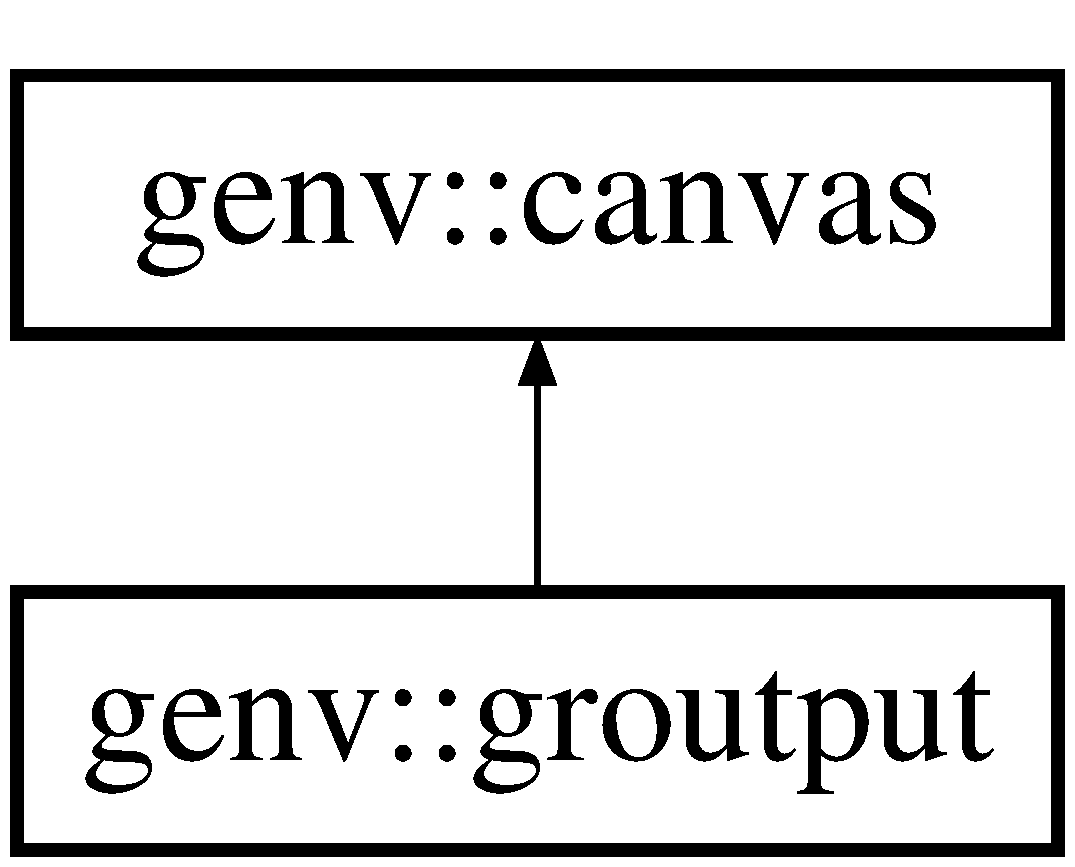
\includegraphics[height=2.000000cm]{classgenv_1_1groutput}
\end{center}
\end{figure}
\subsection*{Publikus tagfüggvények}
\begin{DoxyCompactItemize}
\item 
\mbox{\Hypertarget{classgenv_1_1groutput_a8ed996705e1dc0620715b193c971faf8}\label{classgenv_1_1groutput_a8ed996705e1dc0620715b193c971faf8}} 
void {\bfseries showmouse} (bool toggle)
\item 
\mbox{\Hypertarget{classgenv_1_1groutput_a2d0714199248562a8b0c8124dec148ea}\label{classgenv_1_1groutput_a2d0714199248562a8b0c8124dec148ea}} 
void {\bfseries movemouse} (int x, int y)
\item 
\mbox{\Hypertarget{classgenv_1_1groutput_a4f2e395396c08492e5fb23e63d9d3c77}\label{classgenv_1_1groutput_a4f2e395396c08492e5fb23e63d9d3c77}} 
bool {\bfseries open} (unsigned width, unsigned height, bool fullscreen=false)
\item 
\mbox{\Hypertarget{classgenv_1_1groutput_a5cf426dcd4d104ad23e359e4d8106ad3}\label{classgenv_1_1groutput_a5cf426dcd4d104ad23e359e4d8106ad3}} 
virtual void {\bfseries refresh} ()
\item 
\mbox{\Hypertarget{classgenv_1_1groutput_acb0e52cee139f03f653a8adefc7c31ba}\label{classgenv_1_1groutput_acb0e52cee139f03f653a8adefc7c31ba}} 
void {\bfseries set\+\_\+title} (const std\+::string \&title)
\end{DoxyCompactItemize}
\subsection*{Statikus publikus tagfüggvények}
\begin{DoxyCompactItemize}
\item 
\mbox{\Hypertarget{classgenv_1_1groutput_aaa2dd41fe95e14d04e97c4811dcacf75}\label{classgenv_1_1groutput_aaa2dd41fe95e14d04e97c4811dcacf75}} 
static \hyperlink{classgenv_1_1groutput}{groutput} \& {\bfseries instance} ()
\end{DoxyCompactItemize}
\subsection*{Additional Inherited Members}


Ez a dokumentáció az osztályról a következő fájl alapján készült\+:\begin{DoxyCompactItemize}
\item 
graphics.\+hpp\end{DoxyCompactItemize}

\hypertarget{class_g_u_i_handler}{}\section{G\+U\+I\+Handler osztályreferencia}
\label{class_g_u_i_handler}\index{G\+U\+I\+Handler@{G\+U\+I\+Handler}}
\subsection*{Publikus tagfüggvények}
\begin{DoxyCompactItemize}
\item 
\hyperlink{class_g_u_i_handler_a5f7c105ce1232b512206e7720c91d5e3}{G\+U\+I\+Handler} (int \&xx, int \&yy)
\item 
void \hyperlink{class_g_u_i_handler_ab25716ff908ac3258a11ceff6511c1a8}{Add\+Widget} (\hyperlink{class_widget}{Widget} $\ast$w)
\item 
void \hyperlink{class_g_u_i_handler_a1aab537eafbed97a0b5fc3d766c3a0f8}{Remove\+Widget} (int num)
\item 
void \hyperlink{class_g_u_i_handler_aab8a99ca72267874a44658289b549475}{Remove\+Widget} (\hyperlink{class_widget}{Widget} $\ast$w)
\item 
\mbox{\Hypertarget{class_g_u_i_handler_a37fa59c3f059dbabf71cde6c512ed7a7}\label{class_g_u_i_handler_a37fa59c3f059dbabf71cde6c512ed7a7}} 
void {\bfseries Delete\+All\+Widget} ()
\item 
void \hyperlink{class_g_u_i_handler_a2682b297a7ec68033772358add0b6ca5}{Start} (bool exit\+On\+Escape, int timer)
\item 
\mbox{\Hypertarget{class_g_u_i_handler_ad02a7d1ca919b024bff2c7448eb03b1f}\label{class_g_u_i_handler_ad02a7d1ca919b024bff2c7448eb03b1f}} 
void {\bfseries Exit} ()
\item 
\mbox{\Hypertarget{class_g_u_i_handler_a142790c8f0c34233d839afc497bc0a73}\label{class_g_u_i_handler_a142790c8f0c34233d839afc497bc0a73}} 
bool {\bfseries Get\+Is\+Running} ()
\item 
\mbox{\Hypertarget{class_g_u_i_handler_ae2e564681e3a523af1d66ee17aa1c72c}\label{class_g_u_i_handler_ae2e564681e3a523af1d66ee17aa1c72c}} 
int {\bfseries Get\+Widget\+Number} (\hyperlink{class_widget}{Widget} $\ast$a)
\end{DoxyCompactItemize}
\subsection*{Privát tagfüggvények}
\begin{DoxyCompactItemize}
\item 
void \hyperlink{class_g_u_i_handler_a62e6efe1f011584f34ec69b20b585c18}{Draw} ()
\item 
void \hyperlink{class_g_u_i_handler_a8ea722319827ba27eb941151c562539f}{Handle} (\hyperlink{structgenv_1_1event}{genv\+::event} ev)
\end{DoxyCompactItemize}
\subsection*{Privát attribútumok}
\begin{DoxyCompactItemize}
\item 
std\+::vector$<$ \hyperlink{class_widget}{Widget} $\ast$ $>$ \hyperlink{class_g_u_i_handler_a393237de816334de912d1b113ee1fcc5}{Widgets}
\item 
int \hyperlink{class_g_u_i_handler_ac16356b3284231bdd602f3b0176955fe}{Selected\+Widget}
\item 
\hyperlink{class_colour}{Colour} $\ast$ \hyperlink{class_g_u_i_handler_af084b370233fa8e3bda14b9a35828eb6}{bg\+Colour}
\item 
int \hyperlink{class_g_u_i_handler_ac0cbeb259e73abcbe34888ca5ff4a248}{WindowX}
\item 
int \hyperlink{class_g_u_i_handler_aa4ee4e5b027093bd990e7f06e12c35b5}{WindowY}
\item 
\mbox{\Hypertarget{class_g_u_i_handler_a5dd2d0cb24cf73d4a7487c25a2a13f61}\label{class_g_u_i_handler_a5dd2d0cb24cf73d4a7487c25a2a13f61}} 
bool {\bfseries Exiting}
\item 
\mbox{\Hypertarget{class_g_u_i_handler_a28ce7aa5216fc6082537a0b598aba67e}\label{class_g_u_i_handler_a28ce7aa5216fc6082537a0b598aba67e}} 
bool {\bfseries Is\+Running}
\item 
bool \hyperlink{class_g_u_i_handler_af864fc3eb860de1b198cf857dc120db9}{is\+Escape\+Exit}
\end{DoxyCompactItemize}


\subsection{Konstruktorok és destruktorok dokumentációja}
\mbox{\Hypertarget{class_g_u_i_handler_a5f7c105ce1232b512206e7720c91d5e3}\label{class_g_u_i_handler_a5f7c105ce1232b512206e7720c91d5e3}} 
\index{G\+U\+I\+Handler@{G\+U\+I\+Handler}!G\+U\+I\+Handler@{G\+U\+I\+Handler}}
\index{G\+U\+I\+Handler@{G\+U\+I\+Handler}!G\+U\+I\+Handler@{G\+U\+I\+Handler}}
\subsubsection{\texorpdfstring{G\+U\+I\+Handler()}{GUIHandler()}}
{\footnotesize\ttfamily G\+U\+I\+Handler\+::\+G\+U\+I\+Handler (\begin{DoxyParamCaption}\item[{int \&}]{xx,  }\item[{int \&}]{yy }\end{DoxyParamCaption})}

Ez az oszt�ly kezeli az �sszes widgetet 
\begin{DoxyParams}{Paraméterek}
{\em xx} & az ablak sz�less�ge \\
\hline
{\em yy} & az ablak magass�ga \\
\hline
\end{DoxyParams}


\subsection{Tagfüggvények dokumentációja}
\mbox{\Hypertarget{class_g_u_i_handler_ab25716ff908ac3258a11ceff6511c1a8}\label{class_g_u_i_handler_ab25716ff908ac3258a11ceff6511c1a8}} 
\index{G\+U\+I\+Handler@{G\+U\+I\+Handler}!Add\+Widget@{Add\+Widget}}
\index{Add\+Widget@{Add\+Widget}!G\+U\+I\+Handler@{G\+U\+I\+Handler}}
\subsubsection{\texorpdfstring{Add\+Widget()}{AddWidget()}}
{\footnotesize\ttfamily void G\+U\+I\+Handler\+::\+Add\+Widget (\begin{DoxyParamCaption}\item[{\hyperlink{class_widget}{Widget} $\ast$}]{w }\end{DoxyParamCaption})}

Ezzel a f�ggvv�nnyel lehet �j widgetet hozz�dani az oszt�lyhoz 
\begin{DoxyParams}{Paraméterek}
{\em w} & egy mutat� a hozz�dani k�v�nt widgetre \\
\hline
\end{DoxyParams}
\mbox{\Hypertarget{class_g_u_i_handler_a62e6efe1f011584f34ec69b20b585c18}\label{class_g_u_i_handler_a62e6efe1f011584f34ec69b20b585c18}} 
\index{G\+U\+I\+Handler@{G\+U\+I\+Handler}!Draw@{Draw}}
\index{Draw@{Draw}!G\+U\+I\+Handler@{G\+U\+I\+Handler}}
\subsubsection{\texorpdfstring{Draw()}{Draw()}}
{\footnotesize\ttfamily void G\+U\+I\+Handler\+::\+Draw (\begin{DoxyParamCaption}{ }\end{DoxyParamCaption})\hspace{0.3cm}{\ttfamily [private]}}

Ez a f�ggv�ny felel a k�perny� t�rl�s��rt �s a widgetek kirajzol�s��rt \mbox{\Hypertarget{class_g_u_i_handler_a8ea722319827ba27eb941151c562539f}\label{class_g_u_i_handler_a8ea722319827ba27eb941151c562539f}} 
\index{G\+U\+I\+Handler@{G\+U\+I\+Handler}!Handle@{Handle}}
\index{Handle@{Handle}!G\+U\+I\+Handler@{G\+U\+I\+Handler}}
\subsubsection{\texorpdfstring{Handle()}{Handle()}}
{\footnotesize\ttfamily void G\+U\+I\+Handler\+::\+Handle (\begin{DoxyParamCaption}\item[{\hyperlink{structgenv_1_1event}{genv\+::event}}]{ev }\end{DoxyParamCaption})\hspace{0.3cm}{\ttfamily [private]}}

Ez a f�ggv�ny kezeli az inputokat 
\begin{DoxyParams}{Paraméterek}
{\em ev} & a megkapott eventet t�rolja \\
\hline
\end{DoxyParams}
\mbox{\Hypertarget{class_g_u_i_handler_a1aab537eafbed97a0b5fc3d766c3a0f8}\label{class_g_u_i_handler_a1aab537eafbed97a0b5fc3d766c3a0f8}} 
\index{G\+U\+I\+Handler@{G\+U\+I\+Handler}!Remove\+Widget@{Remove\+Widget}}
\index{Remove\+Widget@{Remove\+Widget}!G\+U\+I\+Handler@{G\+U\+I\+Handler}}
\subsubsection{\texorpdfstring{Remove\+Widget()}{RemoveWidget()}\hspace{0.1cm}{\footnotesize\ttfamily [1/2]}}
{\footnotesize\ttfamily void G\+U\+I\+Handler\+::\+Remove\+Widget (\begin{DoxyParamCaption}\item[{int}]{num }\end{DoxyParamCaption})}

Ez a f�ggv�ny az adott poz�cion lev� widgetet t�vol�tja el az oszt�lyb�l, es t�rli a k�perny�r�l 
\begin{DoxyParams}{Paraméterek}
{\em num} & adja meg a vektorban lev� sorsz�m�t a t�r�lni k�v�nt vektornak \\
\hline
\end{DoxyParams}
\mbox{\Hypertarget{class_g_u_i_handler_aab8a99ca72267874a44658289b549475}\label{class_g_u_i_handler_aab8a99ca72267874a44658289b549475}} 
\index{G\+U\+I\+Handler@{G\+U\+I\+Handler}!Remove\+Widget@{Remove\+Widget}}
\index{Remove\+Widget@{Remove\+Widget}!G\+U\+I\+Handler@{G\+U\+I\+Handler}}
\subsubsection{\texorpdfstring{Remove\+Widget()}{RemoveWidget()}\hspace{0.1cm}{\footnotesize\ttfamily [2/2]}}
{\footnotesize\ttfamily void G\+U\+I\+Handler\+::\+Remove\+Widget (\begin{DoxyParamCaption}\item[{\hyperlink{class_widget}{Widget} $\ast$}]{w }\end{DoxyParamCaption})}

Ez a f�ggv�ny t�rli a megadott widgetet az oszt�lyb�l, ha l�tezik 
\begin{DoxyParams}{Paraméterek}
{\em w} & a t�r�lni k�v�nt widget \\
\hline
\end{DoxyParams}
\mbox{\Hypertarget{class_g_u_i_handler_a2682b297a7ec68033772358add0b6ca5}\label{class_g_u_i_handler_a2682b297a7ec68033772358add0b6ca5}} 
\index{G\+U\+I\+Handler@{G\+U\+I\+Handler}!Start@{Start}}
\index{Start@{Start}!G\+U\+I\+Handler@{G\+U\+I\+Handler}}
\subsubsection{\texorpdfstring{Start()}{Start()}}
{\footnotesize\ttfamily void G\+U\+I\+Handler\+::\+Start (\begin{DoxyParamCaption}\item[{bool}]{exit\+On\+Escape,  }\item[{int}]{timer }\end{DoxyParamCaption})}

Ez a f�ggv�ny ind�tja el a f� ciklust ami kezeli az inputot �s a widgeteket 
\begin{DoxyParams}{Paraméterek}
{\em exit\+On\+Escape} & ha igazra van �llitva a grafikus fel�letb�l ki lehet l�pni az Esc billenty� lenyom�s�val \\
\hline
{\em timer} & megadja, hogy h�ny milliszekundomonk�nt rajzolja �jra a k�perny�t \\
\hline
\end{DoxyParams}


\subsection{Adattagok dokumentációja}
\mbox{\Hypertarget{class_g_u_i_handler_af084b370233fa8e3bda14b9a35828eb6}\label{class_g_u_i_handler_af084b370233fa8e3bda14b9a35828eb6}} 
\index{G\+U\+I\+Handler@{G\+U\+I\+Handler}!bg\+Colour@{bg\+Colour}}
\index{bg\+Colour@{bg\+Colour}!G\+U\+I\+Handler@{G\+U\+I\+Handler}}
\subsubsection{\texorpdfstring{bg\+Colour}{bgColour}}
{\footnotesize\ttfamily \hyperlink{class_colour}{Colour}$\ast$ G\+U\+I\+Handler\+::bg\+Colour\hspace{0.3cm}{\ttfamily [private]}}

Ez az ablak h�tt�rsz�n�t adja meg \mbox{\Hypertarget{class_g_u_i_handler_af864fc3eb860de1b198cf857dc120db9}\label{class_g_u_i_handler_af864fc3eb860de1b198cf857dc120db9}} 
\index{G\+U\+I\+Handler@{G\+U\+I\+Handler}!is\+Escape\+Exit@{is\+Escape\+Exit}}
\index{is\+Escape\+Exit@{is\+Escape\+Exit}!G\+U\+I\+Handler@{G\+U\+I\+Handler}}
\subsubsection{\texorpdfstring{is\+Escape\+Exit}{isEscapeExit}}
{\footnotesize\ttfamily bool G\+U\+I\+Handler\+::is\+Escape\+Exit\hspace{0.3cm}{\ttfamily [private]}}

Ezzel ellen�rz�m, hogy ki kell-\/e l�pni az Esc billenty� lenyom�s�ra \mbox{\Hypertarget{class_g_u_i_handler_ac16356b3284231bdd602f3b0176955fe}\label{class_g_u_i_handler_ac16356b3284231bdd602f3b0176955fe}} 
\index{G\+U\+I\+Handler@{G\+U\+I\+Handler}!Selected\+Widget@{Selected\+Widget}}
\index{Selected\+Widget@{Selected\+Widget}!G\+U\+I\+Handler@{G\+U\+I\+Handler}}
\subsubsection{\texorpdfstring{Selected\+Widget}{SelectedWidget}}
{\footnotesize\ttfamily int G\+U\+I\+Handler\+::\+Selected\+Widget\hspace{0.3cm}{\ttfamily [private]}}

Ez az �ppen kiv�lasztott widget sorsz�m�t t�rolja \mbox{\Hypertarget{class_g_u_i_handler_a393237de816334de912d1b113ee1fcc5}\label{class_g_u_i_handler_a393237de816334de912d1b113ee1fcc5}} 
\index{G\+U\+I\+Handler@{G\+U\+I\+Handler}!Widgets@{Widgets}}
\index{Widgets@{Widgets}!G\+U\+I\+Handler@{G\+U\+I\+Handler}}
\subsubsection{\texorpdfstring{Widgets}{Widgets}}
{\footnotesize\ttfamily std\+::vector$<$\hyperlink{class_widget}{Widget}$\ast$$>$ G\+U\+I\+Handler\+::\+Widgets\hspace{0.3cm}{\ttfamily [private]}}

Ez a vektor t�rolja a widgeteket \mbox{\Hypertarget{class_g_u_i_handler_ac0cbeb259e73abcbe34888ca5ff4a248}\label{class_g_u_i_handler_ac0cbeb259e73abcbe34888ca5ff4a248}} 
\index{G\+U\+I\+Handler@{G\+U\+I\+Handler}!WindowX@{WindowX}}
\index{WindowX@{WindowX}!G\+U\+I\+Handler@{G\+U\+I\+Handler}}
\subsubsection{\texorpdfstring{WindowX}{WindowX}}
{\footnotesize\ttfamily int G\+U\+I\+Handler\+::\+WindowX\hspace{0.3cm}{\ttfamily [private]}}

Ebben t�rolom az ablak sz�less�g�t \mbox{\Hypertarget{class_g_u_i_handler_aa4ee4e5b027093bd990e7f06e12c35b5}\label{class_g_u_i_handler_aa4ee4e5b027093bd990e7f06e12c35b5}} 
\index{G\+U\+I\+Handler@{G\+U\+I\+Handler}!WindowY@{WindowY}}
\index{WindowY@{WindowY}!G\+U\+I\+Handler@{G\+U\+I\+Handler}}
\subsubsection{\texorpdfstring{WindowY}{WindowY}}
{\footnotesize\ttfamily int G\+U\+I\+Handler\+::\+WindowY\hspace{0.3cm}{\ttfamily [private]}}

Ebben t�rolom az ablak magass�g�t 

Ez a dokumentáció az osztályról a következő fájlok alapján készült\+:\begin{DoxyCompactItemize}
\item 
G\+U\+I\+Handler.\+h\item 
G\+U\+I\+Handler.\+cpp\end{DoxyCompactItemize}

\hypertarget{class_label}{}\section{Label osztályreferencia}
\label{class_label}\index{Label@{Label}}
A Label osztály származási diagramja\+:\begin{figure}[H]
\begin{center}
\leavevmode
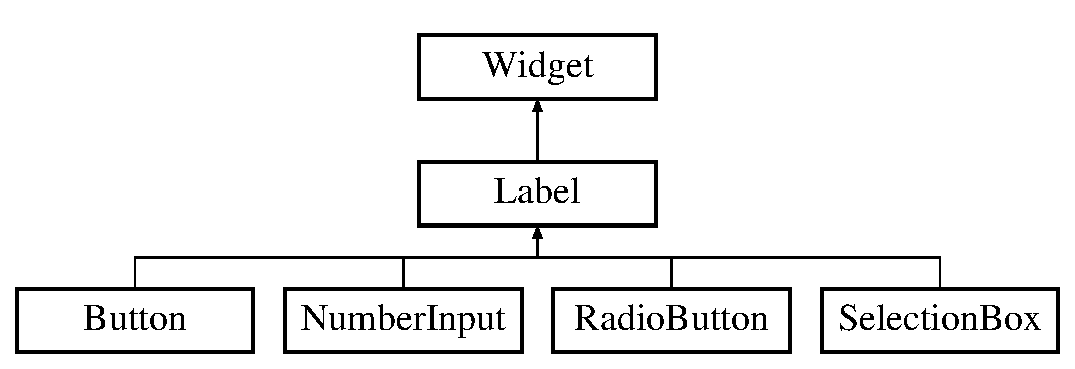
\includegraphics[height=3.000000cm]{class_label}
\end{center}
\end{figure}
\subsection*{Publikus tagfüggvények}
\begin{DoxyCompactItemize}
\item 
\hyperlink{class_label_a4fcabadbd0cfb0a53b8d1caf306bd5a7}{Label} (int x, int y, int x\+Size, int y\+Size, std\+::string \hyperlink{structgenv_1_1text}{text})
\item 
virtual void \hyperlink{class_label_a184df028b3aa8c7f8dec8ecb90533319}{Draw} ()
\item 
virtual void \hyperlink{class_label_a5cf04da7def075453b5c0fda93a1b575}{Handle} (\hyperlink{structgenv_1_1event}{genv\+::event} ev)
\item 
virtual bool \hyperlink{class_label_a918ebb45dbaa5484643355cf5ab4be47}{Is\+In\+Line} (int x, int y)
\item 
bool \hyperlink{class_label_a0dcc047c736b8c20bcba6796e85f909e}{Is\+Text\+Fits} ()
\item 
void \hyperlink{class_label_ac22c98a976f1fb6f4b86ee9ac8dd50b2}{Set\+Font\+Colour} (int r, int g, int b)
\item 
void \hyperlink{class_label_a4dcd2036ce1fdd30eb3471e2c842e97d}{Set\+Text} (std\+::string new\+Text)
\end{DoxyCompactItemize}
\subsection*{Védett attribútumok}
\begin{DoxyCompactItemize}
\item 
\hyperlink{class_colour}{Colour} $\ast$ \hyperlink{class_label_a72057af57385e0e88577cae1ae35af66}{font\+Color}
\item 
std\+::string \hyperlink{class_label_a74410e9b43ea90d40c828008e5904f95}{Text}
\end{DoxyCompactItemize}


\subsection{Konstruktorok és destruktorok dokumentációja}
\mbox{\Hypertarget{class_label_a4fcabadbd0cfb0a53b8d1caf306bd5a7}\label{class_label_a4fcabadbd0cfb0a53b8d1caf306bd5a7}} 
\index{Label@{Label}!Label@{Label}}
\index{Label@{Label}!Label@{Label}}
\subsubsection{\texorpdfstring{Label()}{Label()}}
{\footnotesize\ttfamily Label\+::\+Label (\begin{DoxyParamCaption}\item[{int}]{x,  }\item[{int}]{y,  }\item[{int}]{x\+Size,  }\item[{int}]{y\+Size,  }\item[{std\+::string}]{text }\end{DoxyParamCaption})}

Egy \hyperlink{class_label}{Label} widgetet hoz létre ami egyszerűen egy szöveget tárol és rajzol ki 
\begin{DoxyParams}{Paraméterek}
{\em x} & Az X pozíciót tárolja \\
\hline
{\em y} & Az Y pozíciót tátolja \\
\hline
{\em x\+Size} & Az X tengelyen való hosszt tárolja \\
\hline
{\em y\+Size} & Az Y tengelyen való magasságot tárolja \\
\hline
{\em text} & A kirajzolni kívánt szöveg \\
\hline
\end{DoxyParams}


\subsection{Tagfüggvények dokumentációja}
\mbox{\Hypertarget{class_label_a184df028b3aa8c7f8dec8ecb90533319}\label{class_label_a184df028b3aa8c7f8dec8ecb90533319}} 
\index{Label@{Label}!Draw@{Draw}}
\index{Draw@{Draw}!Label@{Label}}
\subsubsection{\texorpdfstring{Draw()}{Draw()}}
{\footnotesize\ttfamily void Label\+::\+Draw (\begin{DoxyParamCaption}{ }\end{DoxyParamCaption})\hspace{0.3cm}{\ttfamily [virtual]}}

Ez a függvény felel a widget kirajzolásáért 

Megvalósítja a következőket\+: \hyperlink{class_widget_ac4c2063cd671468ad05d84cfe963c032}{Widget}.



Újraimplementáló leszármazottak\+: \hyperlink{class_radio_button_a296e30588da8a4767164c2dfc5d25a71}{Radio\+Button}, \hyperlink{class_number_input_ab65631421ec222bb929f74d1782b5c8b}{Number\+Input}, \hyperlink{class_selection_box_a1c0b7b6c851180450964a4df0c7c15e8}{Selection\+Box} és \hyperlink{class_button_a6aaa2b781c933a296f41a8eca890eb1f}{Button}.

\mbox{\Hypertarget{class_label_a5cf04da7def075453b5c0fda93a1b575}\label{class_label_a5cf04da7def075453b5c0fda93a1b575}} 
\index{Label@{Label}!Handle@{Handle}}
\index{Handle@{Handle}!Label@{Label}}
\subsubsection{\texorpdfstring{Handle()}{Handle()}}
{\footnotesize\ttfamily virtual void Label\+::\+Handle (\begin{DoxyParamCaption}\item[{\hyperlink{structgenv_1_1event}{genv\+::event}}]{ev }\end{DoxyParamCaption})\hspace{0.3cm}{\ttfamily [inline]}, {\ttfamily [virtual]}}

Ez a függvény kezeli az eventeket (ebben az oszályban üres, mivel a \hyperlink{class_label}{Label} csak szöveg kijelzsésére használt) 
\begin{DoxyParams}{Paraméterek}
{\em ev} & Az aktuális event objektum \\
\hline
\end{DoxyParams}


Megvalósítja a következőket\+: \hyperlink{class_widget_abf512e4606c7a5d44245a9b0246634a0}{Widget}.



Újraimplementáló leszármazottak\+: \hyperlink{class_radio_button_a9287d026f57bdfedd878269ec4648135}{Radio\+Button}, \hyperlink{class_button_a72dc68b7a78edfebe904bf489d6e03fb}{Button}, \hyperlink{class_number_input_a08a2de51093fe35c3c7b9998e88924a9}{Number\+Input} és \hyperlink{class_selection_box_a4762480ce86018d74c0cfa271c9cce11}{Selection\+Box}.

\mbox{\Hypertarget{class_label_a918ebb45dbaa5484643355cf5ab4be47}\label{class_label_a918ebb45dbaa5484643355cf5ab4be47}} 
\index{Label@{Label}!Is\+In\+Line@{Is\+In\+Line}}
\index{Is\+In\+Line@{Is\+In\+Line}!Label@{Label}}
\subsubsection{\texorpdfstring{Is\+In\+Line()}{IsInLine()}}
{\footnotesize\ttfamily bool Label\+::\+Is\+In\+Line (\begin{DoxyParamCaption}\item[{int}]{x,  }\item[{int}]{y }\end{DoxyParamCaption})\hspace{0.3cm}{\ttfamily [virtual]}}

Megadja, hogy az egér a saját keretein belül van-\/e 
\begin{DoxyParams}{Paraméterek}
{\em x} & Az egér X pozíciója \\
\hline
{\em y} & Az egér Y pozíciója \\
\hline
\end{DoxyParams}


Megvalósítja a következőket\+: \hyperlink{class_widget_a7a18323ef481add82e5edba5c0c6ec06}{Widget}.



Újraimplementáló leszármazottak\+: \hyperlink{class_radio_button_a94ab27ee37cdd639a185cb746ad7b32f}{Radio\+Button}, \hyperlink{class_button_a61832186fb0cf58c4c1c6fbbe572b61c}{Button}, \hyperlink{class_number_input_af364cc666a41dfa189e024464e4bc317}{Number\+Input} és \hyperlink{class_selection_box_a0378e1ec035f90dd04efac5d6a2c7132}{Selection\+Box}.

\mbox{\Hypertarget{class_label_a0dcc047c736b8c20bcba6796e85f909e}\label{class_label_a0dcc047c736b8c20bcba6796e85f909e}} 
\index{Label@{Label}!Is\+Text\+Fits@{Is\+Text\+Fits}}
\index{Is\+Text\+Fits@{Is\+Text\+Fits}!Label@{Label}}
\subsubsection{\texorpdfstring{Is\+Text\+Fits()}{IsTextFits()}}
{\footnotesize\ttfamily bool Label\+::\+Is\+Text\+Fits (\begin{DoxyParamCaption}{ }\end{DoxyParamCaption})}

Megadja, hogy az éppen tárolt szöveg elfér-\/e a widgeten \begin{DoxyReturn}{Visszatérési érték}
Elfér-\/e a \char`\"{}\+Text\char`\"{} a widgeten 
\end{DoxyReturn}
\mbox{\Hypertarget{class_label_ac22c98a976f1fb6f4b86ee9ac8dd50b2}\label{class_label_ac22c98a976f1fb6f4b86ee9ac8dd50b2}} 
\index{Label@{Label}!Set\+Font\+Colour@{Set\+Font\+Colour}}
\index{Set\+Font\+Colour@{Set\+Font\+Colour}!Label@{Label}}
\subsubsection{\texorpdfstring{Set\+Font\+Colour()}{SetFontColour()}}
{\footnotesize\ttfamily void Label\+::\+Set\+Font\+Colour (\begin{DoxyParamCaption}\item[{int}]{r,  }\item[{int}]{g,  }\item[{int}]{b }\end{DoxyParamCaption})}

Átálítja az betű színét 
\begin{DoxyParams}{Paraméterek}
{\em r} & A betű piros értéke \\
\hline
{\em g} & A betű zöld értéke \\
\hline
{\em b} & A betű kék értéke \\
\hline
\end{DoxyParams}
\mbox{\Hypertarget{class_label_a4dcd2036ce1fdd30eb3471e2c842e97d}\label{class_label_a4dcd2036ce1fdd30eb3471e2c842e97d}} 
\index{Label@{Label}!Set\+Text@{Set\+Text}}
\index{Set\+Text@{Set\+Text}!Label@{Label}}
\subsubsection{\texorpdfstring{Set\+Text()}{SetText()}}
{\footnotesize\ttfamily void Label\+::\+Set\+Text (\begin{DoxyParamCaption}\item[{std\+::string}]{new\+Text }\end{DoxyParamCaption})}

Átálítja az aktuális szöveget 
\begin{DoxyParams}{Paraméterek}
{\em new\+Text} & Az új szöveg \\
\hline
\end{DoxyParams}


\subsection{Adattagok dokumentációja}
\mbox{\Hypertarget{class_label_a72057af57385e0e88577cae1ae35af66}\label{class_label_a72057af57385e0e88577cae1ae35af66}} 
\index{Label@{Label}!font\+Color@{font\+Color}}
\index{font\+Color@{font\+Color}!Label@{Label}}
\subsubsection{\texorpdfstring{font\+Color}{fontColor}}
{\footnotesize\ttfamily \hyperlink{class_colour}{Colour}$\ast$ Label\+::font\+Color\hspace{0.3cm}{\ttfamily [protected]}}

A szöveg színét tárolja \mbox{\Hypertarget{class_label_a74410e9b43ea90d40c828008e5904f95}\label{class_label_a74410e9b43ea90d40c828008e5904f95}} 
\index{Label@{Label}!Text@{Text}}
\index{Text@{Text}!Label@{Label}}
\subsubsection{\texorpdfstring{Text}{Text}}
{\footnotesize\ttfamily std\+::string Label\+::\+Text\hspace{0.3cm}{\ttfamily [protected]}}

Az aktuális szöveget tárolja 

Ez a dokumentáció az osztályról a következő fájlok alapján készült\+:\begin{DoxyCompactItemize}
\item 
Label.\+h\item 
Label.\+cpp\end{DoxyCompactItemize}

\hypertarget{class_level}{}\section{Level osztályreferencia}
\label{class_level}\index{Level@{Level}}
\subsection*{Publikus tagfüggvények}
\begin{DoxyCompactItemize}
\item 
\hyperlink{class_level_ac9a3c078ddbc1fb1e622aeece4b21484}{Level} (int level\+Size, int win)
\begin{DoxyCompactList}\small\item\em L�trehoz egy �j p�ly�t \end{DoxyCompactList}\item 
int \hyperlink{class_level_a49511c05442d904229c8e603e6dfc067}{Get\+Value} (int x, int y)
\begin{DoxyCompactList}\small\item\em Megadja a p�lya egy adott koordin�t�j�n lev� mez� �rt�k�t \end{DoxyCompactList}\item 
int \hyperlink{class_level_a1acfceb6295e1bf3f3dd3b64bd7d38d6}{Value\+To\+Win} ()
\begin{DoxyCompactList}\small\item\em Visszat�r�sk�nt megadja, hogy h�ny pont kell a gy�zelemhez. \end{DoxyCompactList}\item 
int \hyperlink{class_level_a2f77bdcd4cc4536dc2dffbaf05d4db1d}{Get\+Size} ()
\begin{DoxyCompactList}\small\item\em A p�lya m�ret�t adja meg. \end{DoxyCompactList}\item 
void \hyperlink{class_level_a73b6dd3a3e23881ae63c72d4fc7667bf}{Place} (int x, int y, bool x\+Val)
\begin{DoxyCompactList}\small\item\em A megadott koordin�t�kra elhelyez egy �rt�ket. \end{DoxyCompactList}\item 
int \hyperlink{class_level_ae4c2034a22fc8c229b3b0e058d30fc91}{Is\+Game\+Won} ()
\begin{DoxyCompactList}\small\item\em Megadja, hogy megnyerte-\/e valaki a j�t�kot. \end{DoxyCompactList}\item 
void \hyperlink{class_level_a5414deea40ce7604d7df76cc955b803d}{Remove\+Value} (int x, int y)
\begin{DoxyCompactList}\small\item\em Egy adott koordin�t�r�l t�lri az �rt�ket. \end{DoxyCompactList}\item 
bool \hyperlink{class_level_a635da67a86e8a63bf88571dbcf1b4385}{Is\+Area\+Empty} (int x, int y)
\begin{DoxyCompactList}\small\item\em Megadja, hogy egy adott koordin�ta k�r�l �resek-\/e a mez�k \end{DoxyCompactList}\item 
bool \hyperlink{class_level_a520988125e87d13b98b7c42b5e2fe928}{Is\+Level\+Empty} ()
\begin{DoxyCompactList}\small\item\em Megadja, hogy �res-\/e a p�lya. \end{DoxyCompactList}\item 
void \hyperlink{class_level_a743f5fee9bdce09b4ce87ffc2ceca4ce}{Recount} ()
\begin{DoxyCompactList}\small\item\em Megsz�molja, hogy h�ny X �s O van a p�ly�n \end{DoxyCompactList}\item 
void \hyperlink{class_level_abd143fd02f8959207315bdafd0be05ab}{Reset} ()
\begin{DoxyCompactList}\small\item\em Vissza�ll�tja a p�ly�t alap�rtelmezetten �resbe. \end{DoxyCompactList}\item 
int \hyperlink{class_level_aec4f6c6e75283e425a8cd5d52d35e8ee}{Get\+LastX} ()
\begin{DoxyCompactList}\small\item\em Az utolj�ra m�dos�tott mez� x koordin�t�j�t adja vissza. \end{DoxyCompactList}\item 
int \hyperlink{class_level_ae2a8b36cbebe340d8b0495487a3a156a}{Get\+LastY} ()
\begin{DoxyCompactList}\small\item\em Az utolj�ra m�dos�tott mez� y koordin�t�j�t adja vissza. \end{DoxyCompactList}\item 
void \hyperlink{class_level_a3e93b00a83e3a187d02c2b308ad538ed}{Write\+Current\+Position} (std\+::ostream \&writer)
\begin{DoxyCompactList}\small\item\em A megadott m�don ki�rja a p�lya aktu�lis tartalm�t \end{DoxyCompactList}\end{DoxyCompactItemize}
\subsection*{Privát tagfüggvények}
\begin{DoxyCompactItemize}
\item 
int \hyperlink{class_level_a8ad7db518fbe4527ee2c5b329a35c199}{Check\+Area} (int x, int y, int Look\+For)
\begin{DoxyCompactList}\small\item\em Egy ter�leten ellen�rzi, hogy el�g pontja van-\/e a j�t�kosnak a gy�zelemhez. \end{DoxyCompactList}\end{DoxyCompactItemize}
\subsection*{Privát attribútumok}
\begin{DoxyCompactItemize}
\item 
int $\ast$$\ast$ \hyperlink{class_level_ab03146b79cb15288ae8c2a58ca6bcc25}{Level\+Data}
\item 
int \hyperlink{class_level_af58abc7bfaf524e30484170301e184a4}{Size}
\item 
int \hyperlink{class_level_ae88ea518ad018d37fadbe11a1464fb10}{Need\+To\+Win}
\item 
int \hyperlink{class_level_a93b51a4d35d1c29c52eff276e83a9b43}{X\+Count}
\item 
int \hyperlink{class_level_a425f83b38930d2d8b0e3ce115e881e68}{O\+Count}
\item 
int \hyperlink{class_level_acd5302da9e83ba6183f2167c624b2f1e}{LastX}
\item 
int \hyperlink{class_level_a12ed79a812cee4eee19c63a964e7603d}{LastY}
\end{DoxyCompactItemize}


\subsection{Konstruktorok és destruktorok dokumentációja}
\mbox{\Hypertarget{class_level_ac9a3c078ddbc1fb1e622aeece4b21484}\label{class_level_ac9a3c078ddbc1fb1e622aeece4b21484}} 
\index{Level@{Level}!Level@{Level}}
\index{Level@{Level}!Level@{Level}}
\subsubsection{\texorpdfstring{Level()}{Level()}}
{\footnotesize\ttfamily Level\+::\+Level (\begin{DoxyParamCaption}\item[{int}]{level\+Size,  }\item[{int}]{win }\end{DoxyParamCaption})}



L�trehoz egy �j p�ly�t 


\begin{DoxyParams}{Paraméterek}
{\em level\+Size} & int A p�lya m�rete (X$\ast$X) \\
\hline
{\em win} & int A sz�ks�ges pontsz�m a j�t�k megnyer�s�hez \\
\hline
\end{DoxyParams}


\subsection{Tagfüggvények dokumentációja}
\mbox{\Hypertarget{class_level_a8ad7db518fbe4527ee2c5b329a35c199}\label{class_level_a8ad7db518fbe4527ee2c5b329a35c199}} 
\index{Level@{Level}!Check\+Area@{Check\+Area}}
\index{Check\+Area@{Check\+Area}!Level@{Level}}
\subsubsection{\texorpdfstring{Check\+Area()}{CheckArea()}}
{\footnotesize\ttfamily int Level\+::\+Check\+Area (\begin{DoxyParamCaption}\item[{int}]{x,  }\item[{int}]{y,  }\item[{int}]{Look\+For }\end{DoxyParamCaption})\hspace{0.3cm}{\ttfamily [private]}}



Egy ter�leten ellen�rzi, hogy el�g pontja van-\/e a j�t�kosnak a gy�zelemhez. 


\begin{DoxyParams}{Paraméterek}
{\em x} & int A ter�let k�zep�nek x koordin�t�ja \\
\hline
{\em y} & int A ter�let k�zep�nek y koordin�t�ja \\
\hline
{\em Look\+For} & int A j�t�kos, akit figyelni kell \\
\hline
\end{DoxyParams}
\begin{DoxyReturn}{Visszatérési érték}
int Az adott j�t�kos �rt�ke, ha nyert, 0 ha nem 
\end{DoxyReturn}
\mbox{\Hypertarget{class_level_aec4f6c6e75283e425a8cd5d52d35e8ee}\label{class_level_aec4f6c6e75283e425a8cd5d52d35e8ee}} 
\index{Level@{Level}!Get\+LastX@{Get\+LastX}}
\index{Get\+LastX@{Get\+LastX}!Level@{Level}}
\subsubsection{\texorpdfstring{Get\+Last\+X()}{GetLastX()}}
{\footnotesize\ttfamily int Level\+::\+Get\+LastX (\begin{DoxyParamCaption}{ }\end{DoxyParamCaption})}



Az utolj�ra m�dos�tott mez� x koordin�t�j�t adja vissza. 

\begin{DoxyReturn}{Visszatérési érték}
int Az utolj�ra m�dos�tott mez� x koordin�t�ja 
\end{DoxyReturn}
\mbox{\Hypertarget{class_level_ae2a8b36cbebe340d8b0495487a3a156a}\label{class_level_ae2a8b36cbebe340d8b0495487a3a156a}} 
\index{Level@{Level}!Get\+LastY@{Get\+LastY}}
\index{Get\+LastY@{Get\+LastY}!Level@{Level}}
\subsubsection{\texorpdfstring{Get\+Last\+Y()}{GetLastY()}}
{\footnotesize\ttfamily int Level\+::\+Get\+LastY (\begin{DoxyParamCaption}{ }\end{DoxyParamCaption})}



Az utolj�ra m�dos�tott mez� y koordin�t�j�t adja vissza. 

\begin{DoxyReturn}{Visszatérési érték}
int Az utolj�ra m�dos�tott mez� y koordin�t�ja 
\end{DoxyReturn}
\mbox{\Hypertarget{class_level_a2f77bdcd4cc4536dc2dffbaf05d4db1d}\label{class_level_a2f77bdcd4cc4536dc2dffbaf05d4db1d}} 
\index{Level@{Level}!Get\+Size@{Get\+Size}}
\index{Get\+Size@{Get\+Size}!Level@{Level}}
\subsubsection{\texorpdfstring{Get\+Size()}{GetSize()}}
{\footnotesize\ttfamily int Level\+::\+Get\+Size (\begin{DoxyParamCaption}{ }\end{DoxyParamCaption})}



A p�lya m�ret�t adja meg. 

\begin{DoxyReturn}{Visszatérési érték}
int A p�lya m�rete 
\end{DoxyReturn}
\mbox{\Hypertarget{class_level_a49511c05442d904229c8e603e6dfc067}\label{class_level_a49511c05442d904229c8e603e6dfc067}} 
\index{Level@{Level}!Get\+Value@{Get\+Value}}
\index{Get\+Value@{Get\+Value}!Level@{Level}}
\subsubsection{\texorpdfstring{Get\+Value()}{GetValue()}}
{\footnotesize\ttfamily int Level\+::\+Get\+Value (\begin{DoxyParamCaption}\item[{int}]{x,  }\item[{int}]{y }\end{DoxyParamCaption})}



Megadja a p�lya egy adott koordin�t�j�n lev� mez� �rt�k�t 


\begin{DoxyParams}{Paraméterek}
{\em x} & int Az x koordin�ta \\
\hline
{\em y} & int Az y koordin�ta \\
\hline
\end{DoxyParams}
\begin{DoxyReturn}{Visszatérési érték}
int Az x,y koordin�t�n lev� �rt�k 
\end{DoxyReturn}
\mbox{\Hypertarget{class_level_a635da67a86e8a63bf88571dbcf1b4385}\label{class_level_a635da67a86e8a63bf88571dbcf1b4385}} 
\index{Level@{Level}!Is\+Area\+Empty@{Is\+Area\+Empty}}
\index{Is\+Area\+Empty@{Is\+Area\+Empty}!Level@{Level}}
\subsubsection{\texorpdfstring{Is\+Area\+Empty()}{IsAreaEmpty()}}
{\footnotesize\ttfamily bool Level\+::\+Is\+Area\+Empty (\begin{DoxyParamCaption}\item[{int}]{x,  }\item[{int}]{y }\end{DoxyParamCaption})}



Megadja, hogy egy adott koordin�ta k�r�l �resek-\/e a mez�k 


\begin{DoxyParams}{Paraméterek}
{\em x} & int Az x koordin�ta \\
\hline
{\em y} & int Az y koordin�ta \\
\hline
\end{DoxyParams}
\begin{DoxyReturn}{Visszatérési érték}
bool �resek-\/e a mez�k egy inervalumon bel�l 
\end{DoxyReturn}
\mbox{\Hypertarget{class_level_ae4c2034a22fc8c229b3b0e058d30fc91}\label{class_level_ae4c2034a22fc8c229b3b0e058d30fc91}} 
\index{Level@{Level}!Is\+Game\+Won@{Is\+Game\+Won}}
\index{Is\+Game\+Won@{Is\+Game\+Won}!Level@{Level}}
\subsubsection{\texorpdfstring{Is\+Game\+Won()}{IsGameWon()}}
{\footnotesize\ttfamily int Level\+::\+Is\+Game\+Won (\begin{DoxyParamCaption}{ }\end{DoxyParamCaption})}



Megadja, hogy megnyerte-\/e valaki a j�t�kot. 

\begin{DoxyReturn}{Visszatérési érték}
int A j�t�k aktu�lis �llapota sz�mk�nt (-\/1 nincs v�ge, 0 d�ntetlen, 1 x nyert, 2 O nyert) 
\end{DoxyReturn}
\mbox{\Hypertarget{class_level_a520988125e87d13b98b7c42b5e2fe928}\label{class_level_a520988125e87d13b98b7c42b5e2fe928}} 
\index{Level@{Level}!Is\+Level\+Empty@{Is\+Level\+Empty}}
\index{Is\+Level\+Empty@{Is\+Level\+Empty}!Level@{Level}}
\subsubsection{\texorpdfstring{Is\+Level\+Empty()}{IsLevelEmpty()}}
{\footnotesize\ttfamily bool Level\+::\+Is\+Level\+Empty (\begin{DoxyParamCaption}{ }\end{DoxyParamCaption})}



Megadja, hogy �res-\/e a p�lya. 

\begin{DoxyReturn}{Visszatérési érték}
bool �res-\/e a p�lya 
\end{DoxyReturn}
\mbox{\Hypertarget{class_level_a73b6dd3a3e23881ae63c72d4fc7667bf}\label{class_level_a73b6dd3a3e23881ae63c72d4fc7667bf}} 
\index{Level@{Level}!Place@{Place}}
\index{Place@{Place}!Level@{Level}}
\subsubsection{\texorpdfstring{Place()}{Place()}}
{\footnotesize\ttfamily void Level\+::\+Place (\begin{DoxyParamCaption}\item[{int}]{x,  }\item[{int}]{y,  }\item[{bool}]{x\+Val }\end{DoxyParamCaption})}



A megadott koordin�t�kra elhelyez egy �rt�ket. 


\begin{DoxyParams}{Paraméterek}
{\em x} & int Az x koordin�ta \\
\hline
{\em y} & int Az y koordin�ta \\
\hline
{\em x\+Val} & bool Az elhelyezni k�v�nt �rt�k x-\/e \\
\hline
\end{DoxyParams}
\begin{DoxyReturn}{Visszatérési érték}
void 
\end{DoxyReturn}
\mbox{\Hypertarget{class_level_a743f5fee9bdce09b4ce87ffc2ceca4ce}\label{class_level_a743f5fee9bdce09b4ce87ffc2ceca4ce}} 
\index{Level@{Level}!Recount@{Recount}}
\index{Recount@{Recount}!Level@{Level}}
\subsubsection{\texorpdfstring{Recount()}{Recount()}}
{\footnotesize\ttfamily void Level\+::\+Recount (\begin{DoxyParamCaption}{ }\end{DoxyParamCaption})}



Megsz�molja, hogy h�ny X �s O van a p�ly�n 

\begin{DoxyReturn}{Visszatérési érték}
void 
\end{DoxyReturn}
\mbox{\Hypertarget{class_level_a5414deea40ce7604d7df76cc955b803d}\label{class_level_a5414deea40ce7604d7df76cc955b803d}} 
\index{Level@{Level}!Remove\+Value@{Remove\+Value}}
\index{Remove\+Value@{Remove\+Value}!Level@{Level}}
\subsubsection{\texorpdfstring{Remove\+Value()}{RemoveValue()}}
{\footnotesize\ttfamily void Level\+::\+Remove\+Value (\begin{DoxyParamCaption}\item[{int}]{x,  }\item[{int}]{y }\end{DoxyParamCaption})}



Egy adott koordin�t�r�l t�lri az �rt�ket. 


\begin{DoxyParams}{Paraméterek}
{\em x} & int Az x koordin�ta \\
\hline
{\em y} & int Az y koordin�ta \\
\hline
\end{DoxyParams}
\begin{DoxyReturn}{Visszatérési érték}
void 
\end{DoxyReturn}
\mbox{\Hypertarget{class_level_abd143fd02f8959207315bdafd0be05ab}\label{class_level_abd143fd02f8959207315bdafd0be05ab}} 
\index{Level@{Level}!Reset@{Reset}}
\index{Reset@{Reset}!Level@{Level}}
\subsubsection{\texorpdfstring{Reset()}{Reset()}}
{\footnotesize\ttfamily void Level\+::\+Reset (\begin{DoxyParamCaption}{ }\end{DoxyParamCaption})}



Vissza�ll�tja a p�ly�t alap�rtelmezetten �resbe. 

\begin{DoxyReturn}{Visszatérési érték}
void 
\end{DoxyReturn}
\mbox{\Hypertarget{class_level_a1acfceb6295e1bf3f3dd3b64bd7d38d6}\label{class_level_a1acfceb6295e1bf3f3dd3b64bd7d38d6}} 
\index{Level@{Level}!Value\+To\+Win@{Value\+To\+Win}}
\index{Value\+To\+Win@{Value\+To\+Win}!Level@{Level}}
\subsubsection{\texorpdfstring{Value\+To\+Win()}{ValueToWin()}}
{\footnotesize\ttfamily int Level\+::\+Value\+To\+Win (\begin{DoxyParamCaption}{ }\end{DoxyParamCaption})}



Visszat�r�sk�nt megadja, hogy h�ny pont kell a gy�zelemhez. 

\begin{DoxyReturn}{Visszatérési érték}
int Pontok sz�ma a gy�zelemhez 
\end{DoxyReturn}
\mbox{\Hypertarget{class_level_a3e93b00a83e3a187d02c2b308ad538ed}\label{class_level_a3e93b00a83e3a187d02c2b308ad538ed}} 
\index{Level@{Level}!Write\+Current\+Position@{Write\+Current\+Position}}
\index{Write\+Current\+Position@{Write\+Current\+Position}!Level@{Level}}
\subsubsection{\texorpdfstring{Write\+Current\+Position()}{WriteCurrentPosition()}}
{\footnotesize\ttfamily void Level\+::\+Write\+Current\+Position (\begin{DoxyParamCaption}\item[{std\+::ostream \&}]{writer }\end{DoxyParamCaption})}



A megadott m�don ki�rja a p�lya aktu�lis tartalm�t 


\begin{DoxyParams}{Paraméterek}
{\em writer} & std\+::ostream\& A kimeneti forr�s \\
\hline
\end{DoxyParams}
\begin{DoxyReturn}{Visszatérési érték}
void 
\end{DoxyReturn}


\subsection{Adattagok dokumentációja}
\mbox{\Hypertarget{class_level_acd5302da9e83ba6183f2167c624b2f1e}\label{class_level_acd5302da9e83ba6183f2167c624b2f1e}} 
\index{Level@{Level}!LastX@{LastX}}
\index{LastX@{LastX}!Level@{Level}}
\subsubsection{\texorpdfstring{LastX}{LastX}}
{\footnotesize\ttfamily int Level\+::\+LastX\hspace{0.3cm}{\ttfamily [private]}}

Az utolj�ra m�dos�tott mez� X koordin�t�ja \mbox{\Hypertarget{class_level_a12ed79a812cee4eee19c63a964e7603d}\label{class_level_a12ed79a812cee4eee19c63a964e7603d}} 
\index{Level@{Level}!LastY@{LastY}}
\index{LastY@{LastY}!Level@{Level}}
\subsubsection{\texorpdfstring{LastY}{LastY}}
{\footnotesize\ttfamily int Level\+::\+LastY\hspace{0.3cm}{\ttfamily [private]}}

Az utolj�ra m�dos�tott mez� Y koordin�t�ja \mbox{\Hypertarget{class_level_ab03146b79cb15288ae8c2a58ca6bcc25}\label{class_level_ab03146b79cb15288ae8c2a58ca6bcc25}} 
\index{Level@{Level}!Level\+Data@{Level\+Data}}
\index{Level\+Data@{Level\+Data}!Level@{Level}}
\subsubsection{\texorpdfstring{Level\+Data}{LevelData}}
{\footnotesize\ttfamily int$\ast$$\ast$ Level\+::\+Level\+Data\hspace{0.3cm}{\ttfamily [private]}}

Maga a p�lya adatai \mbox{\Hypertarget{class_level_ae88ea518ad018d37fadbe11a1464fb10}\label{class_level_ae88ea518ad018d37fadbe11a1464fb10}} 
\index{Level@{Level}!Need\+To\+Win@{Need\+To\+Win}}
\index{Need\+To\+Win@{Need\+To\+Win}!Level@{Level}}
\subsubsection{\texorpdfstring{Need\+To\+Win}{NeedToWin}}
{\footnotesize\ttfamily int Level\+::\+Need\+To\+Win\hspace{0.3cm}{\ttfamily [private]}}

A nyer�shet sz�ks�ges pontsz�m \mbox{\Hypertarget{class_level_a425f83b38930d2d8b0e3ce115e881e68}\label{class_level_a425f83b38930d2d8b0e3ce115e881e68}} 
\index{Level@{Level}!O\+Count@{O\+Count}}
\index{O\+Count@{O\+Count}!Level@{Level}}
\subsubsection{\texorpdfstring{O\+Count}{OCount}}
{\footnotesize\ttfamily int Level\+::\+O\+Count\hspace{0.3cm}{\ttfamily [private]}}

O-\/k sz�ma \mbox{\Hypertarget{class_level_af58abc7bfaf524e30484170301e184a4}\label{class_level_af58abc7bfaf524e30484170301e184a4}} 
\index{Level@{Level}!Size@{Size}}
\index{Size@{Size}!Level@{Level}}
\subsubsection{\texorpdfstring{Size}{Size}}
{\footnotesize\ttfamily int Level\+::\+Size\hspace{0.3cm}{\ttfamily [private]}}

A p�lya m�rete \mbox{\Hypertarget{class_level_a93b51a4d35d1c29c52eff276e83a9b43}\label{class_level_a93b51a4d35d1c29c52eff276e83a9b43}} 
\index{Level@{Level}!X\+Count@{X\+Count}}
\index{X\+Count@{X\+Count}!Level@{Level}}
\subsubsection{\texorpdfstring{X\+Count}{XCount}}
{\footnotesize\ttfamily int Level\+::\+X\+Count\hspace{0.3cm}{\ttfamily [private]}}

X-\/ek sz�ma 

Ez a dokumentáció az osztályról a következő fájlok alapján készült\+:\begin{DoxyCompactItemize}
\item 
Level.\+h\item 
Level.\+cpp\end{DoxyCompactItemize}

\hypertarget{structgenv_1_1line}{}\section{genv\+:\+:line struktúrareferencia}
\label{structgenv_1_1line}\index{genv\+::line@{genv\+::line}}
\subsection*{Publikus tagfüggvények}
\begin{DoxyCompactItemize}
\item 
\mbox{\Hypertarget{structgenv_1_1line_a839928e1404ac5125c9e764afcf0141d}\label{structgenv_1_1line_a839928e1404ac5125c9e764afcf0141d}} 
{\bfseries line} (int x, int y)
\item 
\mbox{\Hypertarget{structgenv_1_1line_a51d0a1c02f83cd2c6426cd7491720a11}\label{structgenv_1_1line_a51d0a1c02f83cd2c6426cd7491720a11}} 
void {\bfseries operator()} (\hyperlink{classgenv_1_1canvas}{canvas} \&out)
\end{DoxyCompactItemize}
\subsection*{Publikus attribútumok}
\begin{DoxyCompactItemize}
\item 
\mbox{\Hypertarget{structgenv_1_1line_ab046213bb8b41da64ff5e28074ee15ed}\label{structgenv_1_1line_ab046213bb8b41da64ff5e28074ee15ed}} 
int {\bfseries vec\+\_\+x}
\item 
\mbox{\Hypertarget{structgenv_1_1line_aaa258c38b2e4843a137b358f9a100ff9}\label{structgenv_1_1line_aaa258c38b2e4843a137b358f9a100ff9}} 
int {\bfseries vec\+\_\+y}
\end{DoxyCompactItemize}


Ez a dokumentáció a struktúráról a következő fájl alapján készült\+:\begin{DoxyCompactItemize}
\item 
graphics.\+hpp\end{DoxyCompactItemize}

\hypertarget{structgenv_1_1line__to}{}\section{genv\+:\+:line\+\_\+to struktúrareferencia}
\label{structgenv_1_1line__to}\index{genv\+::line\+\_\+to@{genv\+::line\+\_\+to}}
\subsection*{Publikus tagfüggvények}
\begin{DoxyCompactItemize}
\item 
\mbox{\Hypertarget{structgenv_1_1line__to_ad4542f2b1357a1d357c545682d2ba789}\label{structgenv_1_1line__to_ad4542f2b1357a1d357c545682d2ba789}} 
{\bfseries line\+\_\+to} (unsigned x, unsigned y)
\item 
\mbox{\Hypertarget{structgenv_1_1line__to_ad259d328a81ecb6a4558fa1d2566ef52}\label{structgenv_1_1line__to_ad259d328a81ecb6a4558fa1d2566ef52}} 
void {\bfseries operator()} (\hyperlink{classgenv_1_1canvas}{canvas} \&out)
\end{DoxyCompactItemize}
\subsection*{Publikus attribútumok}
\begin{DoxyCompactItemize}
\item 
\mbox{\Hypertarget{structgenv_1_1line__to_add7d097d37d289d5a8edc9204e129bd5}\label{structgenv_1_1line__to_add7d097d37d289d5a8edc9204e129bd5}} 
int {\bfseries pos\+\_\+x}
\item 
\mbox{\Hypertarget{structgenv_1_1line__to_a30ebc3a8b9f60695f96aad5da4e24a86}\label{structgenv_1_1line__to_a30ebc3a8b9f60695f96aad5da4e24a86}} 
int {\bfseries pos\+\_\+y}
\end{DoxyCompactItemize}


Ez a dokumentáció a struktúráról a következő fájl alapján készült\+:\begin{DoxyCompactItemize}
\item 
graphics.\+hpp\end{DoxyCompactItemize}

\hypertarget{class_min_max}{}\section{Min\+Max osztályreferencia}
\label{class_min_max}\index{Min\+Max@{Min\+Max}}
\subsection*{Publikus tagfüggvények}
\begin{DoxyCompactItemize}
\item 
\hyperlink{class_min_max_a15fb56ebb61d033eced1ae2ae43252a9}{Min\+Max} (int deep, \hyperlink{class_level}{Level} $\ast$current\+Level, bool isX)
\begin{DoxyCompactList}\small\item\em Létrehoz egy új Mini\+Max algoritmus alapján működő számítógépes játékost. \end{DoxyCompactList}\item 
void \hyperlink{class_min_max_a8448a9ea304b2890ddca4a123de5693b}{Step} ()
\begin{DoxyCompactList}\small\item\em Ez a funckció számolja ki a következõ lépését a Mini\+Max algoritmusnak. \end{DoxyCompactList}\end{DoxyCompactItemize}
\subsection*{Privát tagfüggvények}
\begin{DoxyCompactItemize}
\item 
\hyperlink{struct_step_data}{Step\+Data} \hyperlink{class_min_max_ab491c411792412ad53665cbce23c0286}{Next\+Step} (int deep, bool is\+AI)
\begin{DoxyCompactList}\small\item\em Ez a függvény számolja a következõ lépést, úgy hogy rekurzívan meghívja önmagát. \end{DoxyCompactList}\item 
\mbox{\Hypertarget{class_min_max_a80ae5176daca604a8a949a9a03c10036}\label{class_min_max_a80ae5176daca604a8a949a9a03c10036}} 
void {\bfseries Copy\+Levels} ()
\end{DoxyCompactItemize}
\subsection*{Privát attribútumok}
\begin{DoxyCompactItemize}
\item 
bool \hyperlink{class_min_max_a6da4ca45e19de6c1bdbe8a5a3d4b7da8}{IsX}
\item 
\hyperlink{class_level}{Level} $\ast$ \hyperlink{class_min_max_a6972ddd2c6a41089c586220563e07e25}{playing\+Level}
\item 
\hyperlink{class_level}{Level} $\ast$ \hyperlink{class_min_max_a2b1b3631d9cf8c6efec0c7bf16c7d846}{computing\+Level}
\item 
int \hyperlink{class_min_max_a9bb13756ec099292e262724f16d39a88}{Max\+Steps}
\item 
int \hyperlink{class_min_max_ab1a2e347bd948d37b96a6694e6ee4a5b}{Map\+Size}
\item 
\mbox{\Hypertarget{class_min_max_a0740177bb8a63569fca8a05f880d912f}\label{class_min_max_a0740177bb8a63569fca8a05f880d912f}} 
std\+::ofstream {\bfseries Writer}
\end{DoxyCompactItemize}


\subsection{Konstruktorok és destruktorok dokumentációja}
\mbox{\Hypertarget{class_min_max_a15fb56ebb61d033eced1ae2ae43252a9}\label{class_min_max_a15fb56ebb61d033eced1ae2ae43252a9}} 
\index{Min\+Max@{Min\+Max}!Min\+Max@{Min\+Max}}
\index{Min\+Max@{Min\+Max}!Min\+Max@{Min\+Max}}
\subsubsection{\texorpdfstring{Min\+Max()}{MinMax()}}
{\footnotesize\ttfamily Min\+Max\+::\+Min\+Max (\begin{DoxyParamCaption}\item[{int}]{deep,  }\item[{\hyperlink{class_level}{Level} $\ast$}]{current\+Level,  }\item[{bool}]{isX }\end{DoxyParamCaption})}



Létrehoz egy új Mini\+Max algoritmus alapján működő számítógépes játékost. 


\begin{DoxyParams}{Paraméterek}
{\em deep} & int Ezzel lehet megadni, hogy maximum hány lépést számoljon előre \\
\hline
{\em current\+Level} & Level$\ast$ Ez a aktuális pályára mutató mutató \\
\hline
{\em isX} & bool Ez adja meg, hogy a gépi játékos az X-\/el játszik-\/e \\
\hline
\end{DoxyParams}


\subsection{Tagfüggvények dokumentációja}
\mbox{\Hypertarget{class_min_max_ab491c411792412ad53665cbce23c0286}\label{class_min_max_ab491c411792412ad53665cbce23c0286}} 
\index{Min\+Max@{Min\+Max}!Next\+Step@{Next\+Step}}
\index{Next\+Step@{Next\+Step}!Min\+Max@{Min\+Max}}
\subsubsection{\texorpdfstring{Next\+Step()}{NextStep()}}
{\footnotesize\ttfamily \hyperlink{struct_step_data}{Step\+Data} Min\+Max\+::\+Next\+Step (\begin{DoxyParamCaption}\item[{int}]{deep,  }\item[{bool}]{is\+AI }\end{DoxyParamCaption})\hspace{0.3cm}{\ttfamily [private]}}



Ez a függvény számolja a következõ lépést, úgy hogy rekurzívan meghívja önmagát. 


\begin{DoxyParams}{Paraméterek}
{\em deep} & int Az aktuális érték, hogy hány lépést számolt elõre \\
\hline
{\em is\+AI} & bool Megadja, hogy az aktuális lépés neki tesz jót, vagy a játékosnal \\
\hline
\end{DoxyParams}
\begin{DoxyReturn}{Visszatérési érték}
\hyperlink{struct_step_data}{Step\+Data} Megadja a lépés helyét, és a maximálisan szerzett pontot 
\end{DoxyReturn}
\mbox{\Hypertarget{class_min_max_a8448a9ea304b2890ddca4a123de5693b}\label{class_min_max_a8448a9ea304b2890ddca4a123de5693b}} 
\index{Min\+Max@{Min\+Max}!Step@{Step}}
\index{Step@{Step}!Min\+Max@{Min\+Max}}
\subsubsection{\texorpdfstring{Step()}{Step()}}
{\footnotesize\ttfamily void Min\+Max\+::\+Step (\begin{DoxyParamCaption}{ }\end{DoxyParamCaption})}



Ez a funckció számolja ki a következõ lépését a Mini\+Max algoritmusnak. 

\begin{DoxyReturn}{Visszatérési érték}
void 
\end{DoxyReturn}


\subsection{Adattagok dokumentációja}
\mbox{\Hypertarget{class_min_max_a2b1b3631d9cf8c6efec0c7bf16c7d846}\label{class_min_max_a2b1b3631d9cf8c6efec0c7bf16c7d846}} 
\index{Min\+Max@{Min\+Max}!computing\+Level@{computing\+Level}}
\index{computing\+Level@{computing\+Level}!Min\+Max@{Min\+Max}}
\subsubsection{\texorpdfstring{computing\+Level}{computingLevel}}
{\footnotesize\ttfamily \hyperlink{class_level}{Level}$\ast$ Min\+Max\+::computing\+Level\hspace{0.3cm}{\ttfamily [private]}}

Ezen a pályán számolja a lépéseit, így nem kell az éles pályán megtenni a próbalépéseket \mbox{\Hypertarget{class_min_max_a6da4ca45e19de6c1bdbe8a5a3d4b7da8}\label{class_min_max_a6da4ca45e19de6c1bdbe8a5a3d4b7da8}} 
\index{Min\+Max@{Min\+Max}!IsX@{IsX}}
\index{IsX@{IsX}!Min\+Max@{Min\+Max}}
\subsubsection{\texorpdfstring{IsX}{IsX}}
{\footnotesize\ttfamily bool Min\+Max\+::\+IsX\hspace{0.3cm}{\ttfamily [private]}}

Ez a változó tárolja, hogy a gép \textquotesingle{}X\textquotesingle{} szerint játszik-\/e \mbox{\Hypertarget{class_min_max_ab1a2e347bd948d37b96a6694e6ee4a5b}\label{class_min_max_ab1a2e347bd948d37b96a6694e6ee4a5b}} 
\index{Min\+Max@{Min\+Max}!Map\+Size@{Map\+Size}}
\index{Map\+Size@{Map\+Size}!Min\+Max@{Min\+Max}}
\subsubsection{\texorpdfstring{Map\+Size}{MapSize}}
{\footnotesize\ttfamily int Min\+Max\+::\+Map\+Size\hspace{0.3cm}{\ttfamily [private]}}

Ez a változó tárolja a pálya méretét, így nem kell újra és újra lekérni \mbox{\Hypertarget{class_min_max_a9bb13756ec099292e262724f16d39a88}\label{class_min_max_a9bb13756ec099292e262724f16d39a88}} 
\index{Min\+Max@{Min\+Max}!Max\+Steps@{Max\+Steps}}
\index{Max\+Steps@{Max\+Steps}!Min\+Max@{Min\+Max}}
\subsubsection{\texorpdfstring{Max\+Steps}{MaxSteps}}
{\footnotesize\ttfamily int Min\+Max\+::\+Max\+Steps\hspace{0.3cm}{\ttfamily [private]}}

Ez a változó adja meg, hogy maximum hány lépést számolhat elõre. Minnél nagyobb annál pontosabban lép, de a számolás hosszúsága exponenciálisan nõ \mbox{\Hypertarget{class_min_max_a6972ddd2c6a41089c586220563e07e25}\label{class_min_max_a6972ddd2c6a41089c586220563e07e25}} 
\index{Min\+Max@{Min\+Max}!playing\+Level@{playing\+Level}}
\index{playing\+Level@{playing\+Level}!Min\+Max@{Min\+Max}}
\subsubsection{\texorpdfstring{playing\+Level}{playingLevel}}
{\footnotesize\ttfamily \hyperlink{class_level}{Level}$\ast$ Min\+Max\+::playing\+Level\hspace{0.3cm}{\ttfamily [private]}}

Ez a mutató mutat a valódi pályára, amin a játék zajlik 

Ez a dokumentáció az osztályról a következő fájlok alapján készült\+:\begin{DoxyCompactItemize}
\item 
Min\+Max.\+h\item 
Min\+Max.\+cpp\end{DoxyCompactItemize}

\hypertarget{structgenv_1_1move}{}\section{genv\+:\+:move struktúrareferencia}
\label{structgenv_1_1move}\index{genv\+::move@{genv\+::move}}
\subsection*{Publikus tagfüggvények}
\begin{DoxyCompactItemize}
\item 
\mbox{\Hypertarget{structgenv_1_1move_afbf98ade6de4261999af994168551615}\label{structgenv_1_1move_afbf98ade6de4261999af994168551615}} 
{\bfseries move} (int x, int y)
\item 
\mbox{\Hypertarget{structgenv_1_1move_ab8dd0ef18914ea6301966162752db392}\label{structgenv_1_1move_ab8dd0ef18914ea6301966162752db392}} 
void {\bfseries operator()} (\hyperlink{classgenv_1_1canvas}{canvas} \&out)
\end{DoxyCompactItemize}
\subsection*{Publikus attribútumok}
\begin{DoxyCompactItemize}
\item 
\mbox{\Hypertarget{structgenv_1_1move_a94403aa1940b3071703da3217bfe300c}\label{structgenv_1_1move_a94403aa1940b3071703da3217bfe300c}} 
int {\bfseries vec\+\_\+x}
\item 
\mbox{\Hypertarget{structgenv_1_1move_ac957a49d9446552a00537db4177c4fb1}\label{structgenv_1_1move_ac957a49d9446552a00537db4177c4fb1}} 
int {\bfseries vec\+\_\+y}
\end{DoxyCompactItemize}


Ez a dokumentáció a struktúráról a következő fájl alapján készült\+:\begin{DoxyCompactItemize}
\item 
graphics.\+hpp\end{DoxyCompactItemize}

\hypertarget{structgenv_1_1move__to}{}\section{genv\+:\+:move\+\_\+to struktúrareferencia}
\label{structgenv_1_1move__to}\index{genv\+::move\+\_\+to@{genv\+::move\+\_\+to}}
\subsection*{Publikus tagfüggvények}
\begin{DoxyCompactItemize}
\item 
\mbox{\Hypertarget{structgenv_1_1move__to_a96daf75da25a8eeb6df3110bdce481a2}\label{structgenv_1_1move__to_a96daf75da25a8eeb6df3110bdce481a2}} 
{\bfseries move\+\_\+to} (unsigned x, unsigned y)
\item 
\mbox{\Hypertarget{structgenv_1_1move__to_a3321ab8a21292730ad46f62d29ef394f}\label{structgenv_1_1move__to_a3321ab8a21292730ad46f62d29ef394f}} 
void {\bfseries operator()} (\hyperlink{classgenv_1_1canvas}{canvas} \&out)
\end{DoxyCompactItemize}
\subsection*{Publikus attribútumok}
\begin{DoxyCompactItemize}
\item 
\mbox{\Hypertarget{structgenv_1_1move__to_acbe6ef0d2eb7a6f27d6028380ab40593}\label{structgenv_1_1move__to_acbe6ef0d2eb7a6f27d6028380ab40593}} 
int {\bfseries pos\+\_\+x}
\item 
\mbox{\Hypertarget{structgenv_1_1move__to_a56bd951bc4a32057eb0e3670d571a0ab}\label{structgenv_1_1move__to_a56bd951bc4a32057eb0e3670d571a0ab}} 
int {\bfseries pos\+\_\+y}
\end{DoxyCompactItemize}


Ez a dokumentáció a struktúráról a következő fájl alapján készült\+:\begin{DoxyCompactItemize}
\item 
graphics.\+hpp\end{DoxyCompactItemize}

\hypertarget{class_number_input}{}\section{Number\+Input osztályreferencia}
\label{class_number_input}\index{Number\+Input@{Number\+Input}}
A Number\+Input osztály származási diagramja\+:\begin{figure}[H]
\begin{center}
\leavevmode
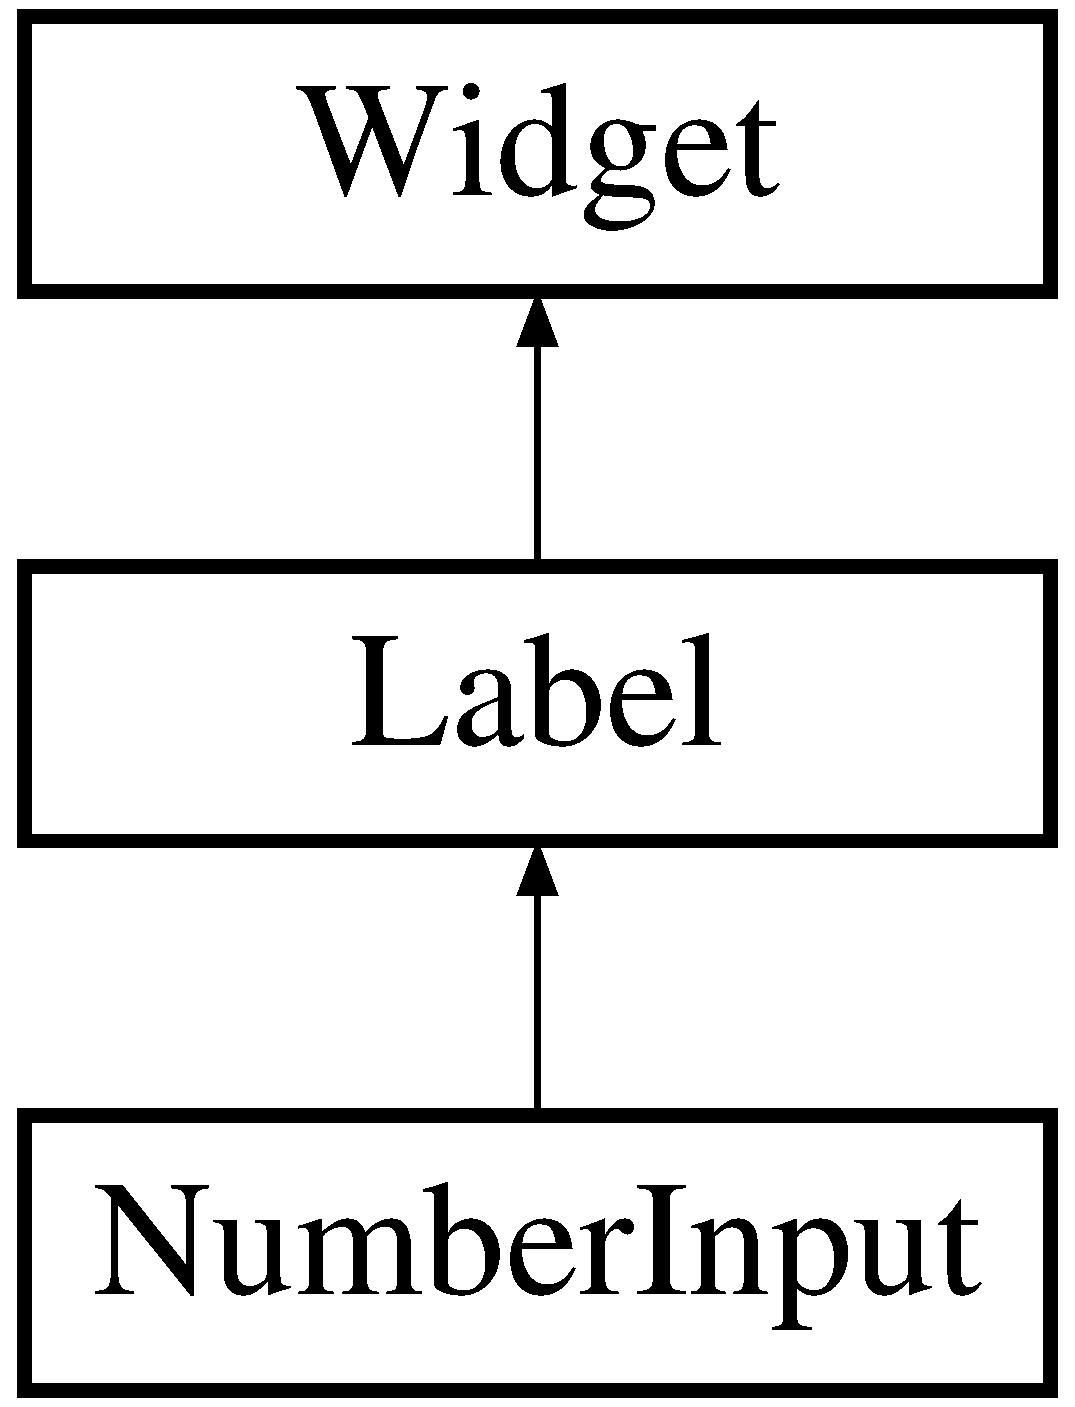
\includegraphics[height=3.000000cm]{class_number_input}
\end{center}
\end{figure}
\subsection*{Publikus tagfüggvények}
\begin{DoxyCompactItemize}
\item 
\hyperlink{class_number_input_aefdfa77f0126ef899ba0a769f2235342}{Number\+Input} (int x, int y, int x\+Size, int y\+Size, int starting\+Number, int max\+Value, int min\+Value)
\item 
void \hyperlink{class_number_input_ab65631421ec222bb929f74d1782b5c8b}{Draw} ()
\item 
void \hyperlink{class_number_input_a08a2de51093fe35c3c7b9998e88924a9}{Handle} (\hyperlink{structgenv_1_1event}{genv\+::event} ev)
\item 
bool \hyperlink{class_number_input_af364cc666a41dfa189e024464e4bc317}{Is\+In\+Line} (int x, int y)
\item 
void \hyperlink{class_number_input_a0682f3a3b5f11c791130dccf93fd99e2}{Set\+Value} (int val)
\item 
void \hyperlink{class_number_input_aef2773ed58e2afdd2db28bcd7adc7502}{Adjust\+Value} (int val)
\item 
void \hyperlink{class_number_input_a9c4d25e738d515215db9e7cf555564e8}{Step} (bool up, bool big)
\item 
void \hyperlink{class_number_input_ae64ca90e8c0aa327c859f0635e534e7e}{Set\+Maximum\+Value} (int maximum)
\item 
void \hyperlink{class_number_input_afd331b555cb1fd5b7b302657970fce7c}{Set\+Minimum\+Value} (int minimum)
\item 
void \hyperlink{class_number_input_acec58e03d46e46cddaab1232ad568321}{Set\+Step\+Value} (int step)
\item 
void \hyperlink{class_number_input_a1697046b4e5612acc5235d0fc641cca3}{Set\+Big\+Step\+Value} (int bigstep)
\item 
void \hyperlink{class_number_input_a2c606ddf06df2f60f26a3e4adaa1dd85}{Set\+Button\+Colour} (int r, int g, int b)
\item 
void \hyperlink{class_number_input_ae7d315b36400c767cff5c29e23504b5a}{Set\+Button\+On\+Click\+Colour} (int r, int g, int b)
\item 
\mbox{\Hypertarget{class_number_input_a4489ce154958175f41d23d1320f982a9}\label{class_number_input_a4489ce154958175f41d23d1320f982a9}} 
int {\bfseries Get\+Current\+Value} ()
\item 
\mbox{\Hypertarget{class_number_input_aabb4deeb84de3beeea983541a1cf6d39}\label{class_number_input_aabb4deeb84de3beeea983541a1cf6d39}} 
void {\bfseries Set\+Event\+Void} (std\+::function$<$ void(\hyperlink{class_number_input}{Number\+Input} $\ast$)$>$ \hyperlink{structgenv_1_1event}{event})
\end{DoxyCompactItemize}
\subsection*{Privát tagfüggvények}
\begin{DoxyCompactItemize}
\item 
void \hyperlink{class_number_input_a1f6bbdba5d2af8b5269d9e00d9d3e1e0}{Check\+Value} ()
\end{DoxyCompactItemize}
\subsection*{Privát attribútumok}
\begin{DoxyCompactItemize}
\item 
int \hyperlink{class_number_input_a95cf7c8f0185f0682a601302a811d2eb}{Current\+Number}
\item 
int \hyperlink{class_number_input_a55812397e1446404f7303b1603f52594}{Maximum\+Value}
\item 
int \hyperlink{class_number_input_af0b3680c0e74abe946bdc888858272fb}{Minimum\+Value}
\item 
int \hyperlink{class_number_input_a22772460b68ff126b8c289290ed09697}{Step\+Value}
\item 
int \hyperlink{class_number_input_a2e2ed204923756a047800cefb9572b6d}{Big\+Step\+Value}
\item 
bool \hyperlink{class_number_input_a0f32b7a17629ee4cf733fc0548ea2e66}{button\+Up\+Clicking}
\item 
bool \hyperlink{class_number_input_a98ab70cc84c3b5d6f134a039cf660f71}{button\+Down\+Clicking}
\item 
\mbox{\Hypertarget{class_number_input_abb2632847adce3030fbb0f5d471a2850}\label{class_number_input_abb2632847adce3030fbb0f5d471a2850}} 
std\+::function$<$ void(\hyperlink{class_number_input}{Number\+Input} $\ast$)$>$ {\bfseries On\+Event}
\item 
\hyperlink{class_colour}{Colour} $\ast$ \hyperlink{class_number_input_a6da104a673a46ff122cb89a5caed6679}{button\+Colour}
\item 
\hyperlink{class_colour}{Colour} $\ast$ \hyperlink{class_number_input_a46fe428af7fba158eb550639a1a5edc9}{button\+Click\+Colour}
\end{DoxyCompactItemize}
\subsection*{Additional Inherited Members}


\subsection{Konstruktorok és destruktorok dokumentációja}
\mbox{\Hypertarget{class_number_input_aefdfa77f0126ef899ba0a769f2235342}\label{class_number_input_aefdfa77f0126ef899ba0a769f2235342}} 
\index{Number\+Input@{Number\+Input}!Number\+Input@{Number\+Input}}
\index{Number\+Input@{Number\+Input}!Number\+Input@{Number\+Input}}
\subsubsection{\texorpdfstring{Number\+Input()}{NumberInput()}}
{\footnotesize\ttfamily Number\+Input\+::\+Number\+Input (\begin{DoxyParamCaption}\item[{int}]{x,  }\item[{int}]{y,  }\item[{int}]{x\+Size,  }\item[{int}]{y\+Size,  }\item[{int}]{starting\+Number,  }\item[{int}]{max\+Value,  }\item[{int}]{min\+Value }\end{DoxyParamCaption})}

Egy sz�ml�l� widget aminek az �rt�ke k�t gombbal, valamint a fel �s le nyilakkal �s a page up, page down gombokkal szab�lyozhat� 
\begin{DoxyParams}{Paraméterek}
{\em x} & A widget X poz�ci�ja \\
\hline
{\em y} & A widget Y poz�ci�ja \\
\hline
{\em x\+Size} & A widget hossza (20 pixel m�g tartozik a v�g�hez, ezek a gombok) \\
\hline
{\em y\+Size} & A widget magass�ga \\
\hline
{\em starting\+Number} & A sz�ml�l� kezd� sz�ma \\
\hline
{\em max\+Value} & A maximum �rt�k, a sz�ml�l� nem mehet ezen t�l \\
\hline
{\em min\+Value} & A minimum �rt�k, a sz�ml�l� �rt�ke nem lehet enn�l kisebb \\
\hline
\end{DoxyParams}


\subsection{Tagfüggvények dokumentációja}
\mbox{\Hypertarget{class_number_input_aef2773ed58e2afdd2db28bcd7adc7502}\label{class_number_input_aef2773ed58e2afdd2db28bcd7adc7502}} 
\index{Number\+Input@{Number\+Input}!Adjust\+Value@{Adjust\+Value}}
\index{Adjust\+Value@{Adjust\+Value}!Number\+Input@{Number\+Input}}
\subsubsection{\texorpdfstring{Adjust\+Value()}{AdjustValue()}}
{\footnotesize\ttfamily void Number\+Input\+::\+Adjust\+Value (\begin{DoxyParamCaption}\item[{int}]{val }\end{DoxyParamCaption})}

Hozz�ad valamennyit a sz�ml�l� jelenlegi �rt�k�hez 
\begin{DoxyParams}{Paraméterek}
{\em val} & A hpzz�adand� �rt�k \\
\hline
\end{DoxyParams}
\mbox{\Hypertarget{class_number_input_a1f6bbdba5d2af8b5269d9e00d9d3e1e0}\label{class_number_input_a1f6bbdba5d2af8b5269d9e00d9d3e1e0}} 
\index{Number\+Input@{Number\+Input}!Check\+Value@{Check\+Value}}
\index{Check\+Value@{Check\+Value}!Number\+Input@{Number\+Input}}
\subsubsection{\texorpdfstring{Check\+Value()}{CheckValue()}}
{\footnotesize\ttfamily void Number\+Input\+::\+Check\+Value (\begin{DoxyParamCaption}{ }\end{DoxyParamCaption})\hspace{0.3cm}{\ttfamily [private]}}

Ellen�rzi, hogy a jelenlegi �rt�k nem-\/e l�g ki a hat�rokon \mbox{\Hypertarget{class_number_input_ab65631421ec222bb929f74d1782b5c8b}\label{class_number_input_ab65631421ec222bb929f74d1782b5c8b}} 
\index{Number\+Input@{Number\+Input}!Draw@{Draw}}
\index{Draw@{Draw}!Number\+Input@{Number\+Input}}
\subsubsection{\texorpdfstring{Draw()}{Draw()}}
{\footnotesize\ttfamily void Number\+Input\+::\+Draw (\begin{DoxyParamCaption}{ }\end{DoxyParamCaption})\hspace{0.3cm}{\ttfamily [virtual]}}

Ez felel a widget kirajzol�s��rt 

Újraimplementált ősök\+: \hyperlink{class_label_a184df028b3aa8c7f8dec8ecb90533319}{Label}.

\mbox{\Hypertarget{class_number_input_a08a2de51093fe35c3c7b9998e88924a9}\label{class_number_input_a08a2de51093fe35c3c7b9998e88924a9}} 
\index{Number\+Input@{Number\+Input}!Handle@{Handle}}
\index{Handle@{Handle}!Number\+Input@{Number\+Input}}
\subsubsection{\texorpdfstring{Handle()}{Handle()}}
{\footnotesize\ttfamily void Number\+Input\+::\+Handle (\begin{DoxyParamCaption}\item[{\hyperlink{structgenv_1_1event}{genv\+::event}}]{ev }\end{DoxyParamCaption})\hspace{0.3cm}{\ttfamily [virtual]}}

Ez a f�ggv�ny kezeli az eventeket 
\begin{DoxyParams}{Paraméterek}
{\em ev} & Az aktu�lis event objektum \\
\hline
\end{DoxyParams}


Újraimplementált ősök\+: \hyperlink{class_label_a5cf04da7def075453b5c0fda93a1b575}{Label}.

\mbox{\Hypertarget{class_number_input_af364cc666a41dfa189e024464e4bc317}\label{class_number_input_af364cc666a41dfa189e024464e4bc317}} 
\index{Number\+Input@{Number\+Input}!Is\+In\+Line@{Is\+In\+Line}}
\index{Is\+In\+Line@{Is\+In\+Line}!Number\+Input@{Number\+Input}}
\subsubsection{\texorpdfstring{Is\+In\+Line()}{IsInLine()}}
{\footnotesize\ttfamily bool Number\+Input\+::\+Is\+In\+Line (\begin{DoxyParamCaption}\item[{int}]{x,  }\item[{int}]{y }\end{DoxyParamCaption})\hspace{0.3cm}{\ttfamily [virtual]}}

Megadja, hogy az eg�r a saj�t keretein bel�l van-\/e 
\begin{DoxyParams}{Paraméterek}
{\em x} & Az eg�r X poz�ci�ja \\
\hline
{\em y} & Az eg�r Y poz�ci�ja \\
\hline
\end{DoxyParams}


Újraimplementált ősök\+: \hyperlink{class_label_a918ebb45dbaa5484643355cf5ab4be47}{Label}.

\mbox{\Hypertarget{class_number_input_a1697046b4e5612acc5235d0fc641cca3}\label{class_number_input_a1697046b4e5612acc5235d0fc641cca3}} 
\index{Number\+Input@{Number\+Input}!Set\+Big\+Step\+Value@{Set\+Big\+Step\+Value}}
\index{Set\+Big\+Step\+Value@{Set\+Big\+Step\+Value}!Number\+Input@{Number\+Input}}
\subsubsection{\texorpdfstring{Set\+Big\+Step\+Value()}{SetBigStepValue()}}
{\footnotesize\ttfamily void Number\+Input\+::\+Set\+Big\+Step\+Value (\begin{DoxyParamCaption}\item[{int}]{bigstep }\end{DoxyParamCaption})}

�t�l�tja a nagy egys�g �rt�k�t (amit a page up/down gombra l�p) 
\begin{DoxyParams}{Paraméterek}
{\em bigstep} & Az �j egys�g �rt�ke \\
\hline
\end{DoxyParams}
\mbox{\Hypertarget{class_number_input_a2c606ddf06df2f60f26a3e4adaa1dd85}\label{class_number_input_a2c606ddf06df2f60f26a3e4adaa1dd85}} 
\index{Number\+Input@{Number\+Input}!Set\+Button\+Colour@{Set\+Button\+Colour}}
\index{Set\+Button\+Colour@{Set\+Button\+Colour}!Number\+Input@{Number\+Input}}
\subsubsection{\texorpdfstring{Set\+Button\+Colour()}{SetButtonColour()}}
{\footnotesize\ttfamily void Number\+Input\+::\+Set\+Button\+Colour (\begin{DoxyParamCaption}\item[{int}]{r,  }\item[{int}]{g,  }\item[{int}]{b }\end{DoxyParamCaption})}

�t�l�tja a gomb sz�n�t 
\begin{DoxyParams}{Paraméterek}
{\em r} & Az �j piros �rt�k \\
\hline
{\em g} & Az �j z�ld �rt�k \\
\hline
{\em b} & Az �j k�k �rt�k \\
\hline
\end{DoxyParams}
\mbox{\Hypertarget{class_number_input_ae7d315b36400c767cff5c29e23504b5a}\label{class_number_input_ae7d315b36400c767cff5c29e23504b5a}} 
\index{Number\+Input@{Number\+Input}!Set\+Button\+On\+Click\+Colour@{Set\+Button\+On\+Click\+Colour}}
\index{Set\+Button\+On\+Click\+Colour@{Set\+Button\+On\+Click\+Colour}!Number\+Input@{Number\+Input}}
\subsubsection{\texorpdfstring{Set\+Button\+On\+Click\+Colour()}{SetButtonOnClickColour()}}
{\footnotesize\ttfamily void Number\+Input\+::\+Set\+Button\+On\+Click\+Colour (\begin{DoxyParamCaption}\item[{int}]{r,  }\item[{int}]{g,  }\item[{int}]{b }\end{DoxyParamCaption})}

�t�l�tja a gomb kattint�skor l�that� sz�n�t 
\begin{DoxyParams}{Paraméterek}
{\em r} & Az �j piros �rt�k \\
\hline
{\em g} & Az �j z�ld �rt�k \\
\hline
{\em b} & Az �j k�k �rt�k \\
\hline
\end{DoxyParams}
\mbox{\Hypertarget{class_number_input_ae64ca90e8c0aa327c859f0635e534e7e}\label{class_number_input_ae64ca90e8c0aa327c859f0635e534e7e}} 
\index{Number\+Input@{Number\+Input}!Set\+Maximum\+Value@{Set\+Maximum\+Value}}
\index{Set\+Maximum\+Value@{Set\+Maximum\+Value}!Number\+Input@{Number\+Input}}
\subsubsection{\texorpdfstring{Set\+Maximum\+Value()}{SetMaximumValue()}}
{\footnotesize\ttfamily void Number\+Input\+::\+Set\+Maximum\+Value (\begin{DoxyParamCaption}\item[{int}]{maximum }\end{DoxyParamCaption})}

�j fels�korl�tot ad a widgetnek 
\begin{DoxyParams}{Paraméterek}
{\em maximum} & Az �j maximum \\
\hline
\end{DoxyParams}
\mbox{\Hypertarget{class_number_input_afd331b555cb1fd5b7b302657970fce7c}\label{class_number_input_afd331b555cb1fd5b7b302657970fce7c}} 
\index{Number\+Input@{Number\+Input}!Set\+Minimum\+Value@{Set\+Minimum\+Value}}
\index{Set\+Minimum\+Value@{Set\+Minimum\+Value}!Number\+Input@{Number\+Input}}
\subsubsection{\texorpdfstring{Set\+Minimum\+Value()}{SetMinimumValue()}}
{\footnotesize\ttfamily void Number\+Input\+::\+Set\+Minimum\+Value (\begin{DoxyParamCaption}\item[{int}]{minimum }\end{DoxyParamCaption})}

�j als�korl�tot ad a widgetnek 
\begin{DoxyParams}{Paraméterek}
{\em minimum} & Az �j minimum \\
\hline
\end{DoxyParams}
\mbox{\Hypertarget{class_number_input_acec58e03d46e46cddaab1232ad568321}\label{class_number_input_acec58e03d46e46cddaab1232ad568321}} 
\index{Number\+Input@{Number\+Input}!Set\+Step\+Value@{Set\+Step\+Value}}
\index{Set\+Step\+Value@{Set\+Step\+Value}!Number\+Input@{Number\+Input}}
\subsubsection{\texorpdfstring{Set\+Step\+Value()}{SetStepValue()}}
{\footnotesize\ttfamily void Number\+Input\+::\+Set\+Step\+Value (\begin{DoxyParamCaption}\item[{int}]{step }\end{DoxyParamCaption})}

�t�l�tja a kis egys�g �rt�k�t (amit egy kattint�ssal l�p) 
\begin{DoxyParams}{Paraméterek}
{\em step} & Az �j egys�g �rt�ke \\
\hline
\end{DoxyParams}
\mbox{\Hypertarget{class_number_input_a0682f3a3b5f11c791130dccf93fd99e2}\label{class_number_input_a0682f3a3b5f11c791130dccf93fd99e2}} 
\index{Number\+Input@{Number\+Input}!Set\+Value@{Set\+Value}}
\index{Set\+Value@{Set\+Value}!Number\+Input@{Number\+Input}}
\subsubsection{\texorpdfstring{Set\+Value()}{SetValue()}}
{\footnotesize\ttfamily void Number\+Input\+::\+Set\+Value (\begin{DoxyParamCaption}\item[{int}]{val }\end{DoxyParamCaption})}

�t�l�tja a sz�ml�l� �rt�k�t 
\begin{DoxyParams}{Paraméterek}
{\em val} & Az �j �rt�k \\
\hline
\end{DoxyParams}
\mbox{\Hypertarget{class_number_input_a9c4d25e738d515215db9e7cf555564e8}\label{class_number_input_a9c4d25e738d515215db9e7cf555564e8}} 
\index{Number\+Input@{Number\+Input}!Step@{Step}}
\index{Step@{Step}!Number\+Input@{Number\+Input}}
\subsubsection{\texorpdfstring{Step()}{Step()}}
{\footnotesize\ttfamily void Number\+Input\+::\+Step (\begin{DoxyParamCaption}\item[{bool}]{up,  }\item[{bool}]{big }\end{DoxyParamCaption})}

A sz�ml�l�t l�pteti kis vagy nagy egys�gnyivel pozit�v vagy negat�v ir�nyba 
\begin{DoxyParams}{Paraméterek}
{\em up} & Ez adja meg, hogy pozit�v ir�nyba l�p-\/e \\
\hline
{\em bug} & Ez adja meg, hogy kis vagy nagy egys�get l�p \\
\hline
\end{DoxyParams}


\subsection{Adattagok dokumentációja}
\mbox{\Hypertarget{class_number_input_a2e2ed204923756a047800cefb9572b6d}\label{class_number_input_a2e2ed204923756a047800cefb9572b6d}} 
\index{Number\+Input@{Number\+Input}!Big\+Step\+Value@{Big\+Step\+Value}}
\index{Big\+Step\+Value@{Big\+Step\+Value}!Number\+Input@{Number\+Input}}
\subsubsection{\texorpdfstring{Big\+Step\+Value}{BigStepValue}}
{\footnotesize\ttfamily int Number\+Input\+::\+Big\+Step\+Value\hspace{0.3cm}{\ttfamily [private]}}

A nagy l�p�s m�rt�ke \mbox{\Hypertarget{class_number_input_a46fe428af7fba158eb550639a1a5edc9}\label{class_number_input_a46fe428af7fba158eb550639a1a5edc9}} 
\index{Number\+Input@{Number\+Input}!button\+Click\+Colour@{button\+Click\+Colour}}
\index{button\+Click\+Colour@{button\+Click\+Colour}!Number\+Input@{Number\+Input}}
\subsubsection{\texorpdfstring{button\+Click\+Colour}{buttonClickColour}}
{\footnotesize\ttfamily \hyperlink{class_colour}{Colour}$\ast$ Number\+Input\+::button\+Click\+Colour\hspace{0.3cm}{\ttfamily [private]}}

A gomb kattint�skor l�that� sz�n�t t�rolja \mbox{\Hypertarget{class_number_input_a6da104a673a46ff122cb89a5caed6679}\label{class_number_input_a6da104a673a46ff122cb89a5caed6679}} 
\index{Number\+Input@{Number\+Input}!button\+Colour@{button\+Colour}}
\index{button\+Colour@{button\+Colour}!Number\+Input@{Number\+Input}}
\subsubsection{\texorpdfstring{button\+Colour}{buttonColour}}
{\footnotesize\ttfamily \hyperlink{class_colour}{Colour}$\ast$ Number\+Input\+::button\+Colour\hspace{0.3cm}{\ttfamily [private]}}

A gomb sz�n�t t�rolja \mbox{\Hypertarget{class_number_input_a98ab70cc84c3b5d6f134a039cf660f71}\label{class_number_input_a98ab70cc84c3b5d6f134a039cf660f71}} 
\index{Number\+Input@{Number\+Input}!button\+Down\+Clicking@{button\+Down\+Clicking}}
\index{button\+Down\+Clicking@{button\+Down\+Clicking}!Number\+Input@{Number\+Input}}
\subsubsection{\texorpdfstring{button\+Down\+Clicking}{buttonDownClicking}}
{\footnotesize\ttfamily bool Number\+Input\+::button\+Down\+Clicking\hspace{0.3cm}{\ttfamily [private]}}

Igaz, amennyiben a lefele gombra �ppen r�kattintanak \mbox{\Hypertarget{class_number_input_a0f32b7a17629ee4cf733fc0548ea2e66}\label{class_number_input_a0f32b7a17629ee4cf733fc0548ea2e66}} 
\index{Number\+Input@{Number\+Input}!button\+Up\+Clicking@{button\+Up\+Clicking}}
\index{button\+Up\+Clicking@{button\+Up\+Clicking}!Number\+Input@{Number\+Input}}
\subsubsection{\texorpdfstring{button\+Up\+Clicking}{buttonUpClicking}}
{\footnotesize\ttfamily bool Number\+Input\+::button\+Up\+Clicking\hspace{0.3cm}{\ttfamily [private]}}

Igaz, amennyiben a felfele gombra �ppen r�kattintanak \mbox{\Hypertarget{class_number_input_a95cf7c8f0185f0682a601302a811d2eb}\label{class_number_input_a95cf7c8f0185f0682a601302a811d2eb}} 
\index{Number\+Input@{Number\+Input}!Current\+Number@{Current\+Number}}
\index{Current\+Number@{Current\+Number}!Number\+Input@{Number\+Input}}
\subsubsection{\texorpdfstring{Current\+Number}{CurrentNumber}}
{\footnotesize\ttfamily int Number\+Input\+::\+Current\+Number\hspace{0.3cm}{\ttfamily [private]}}

A jelenlegi �rt�k \mbox{\Hypertarget{class_number_input_a55812397e1446404f7303b1603f52594}\label{class_number_input_a55812397e1446404f7303b1603f52594}} 
\index{Number\+Input@{Number\+Input}!Maximum\+Value@{Maximum\+Value}}
\index{Maximum\+Value@{Maximum\+Value}!Number\+Input@{Number\+Input}}
\subsubsection{\texorpdfstring{Maximum\+Value}{MaximumValue}}
{\footnotesize\ttfamily int Number\+Input\+::\+Maximum\+Value\hspace{0.3cm}{\ttfamily [private]}}

A maximum �rt�k \mbox{\Hypertarget{class_number_input_af0b3680c0e74abe946bdc888858272fb}\label{class_number_input_af0b3680c0e74abe946bdc888858272fb}} 
\index{Number\+Input@{Number\+Input}!Minimum\+Value@{Minimum\+Value}}
\index{Minimum\+Value@{Minimum\+Value}!Number\+Input@{Number\+Input}}
\subsubsection{\texorpdfstring{Minimum\+Value}{MinimumValue}}
{\footnotesize\ttfamily int Number\+Input\+::\+Minimum\+Value\hspace{0.3cm}{\ttfamily [private]}}

A minimum �rt�k \mbox{\Hypertarget{class_number_input_a22772460b68ff126b8c289290ed09697}\label{class_number_input_a22772460b68ff126b8c289290ed09697}} 
\index{Number\+Input@{Number\+Input}!Step\+Value@{Step\+Value}}
\index{Step\+Value@{Step\+Value}!Number\+Input@{Number\+Input}}
\subsubsection{\texorpdfstring{Step\+Value}{StepValue}}
{\footnotesize\ttfamily int Number\+Input\+::\+Step\+Value\hspace{0.3cm}{\ttfamily [private]}}

A kis l�p�s m�rt�ke 

Ez a dokumentáció az osztályról a következő fájlok alapján készült\+:\begin{DoxyCompactItemize}
\item 
Number\+Input.\+h\item 
Number\+Input.\+cpp\end{DoxyCompactItemize}

\hypertarget{class_radio_button}{}\section{Radio\+Button osztályreferencia}
\label{class_radio_button}\index{Radio\+Button@{Radio\+Button}}
A Radio\+Button osztály származási diagramja\+:\begin{figure}[H]
\begin{center}
\leavevmode
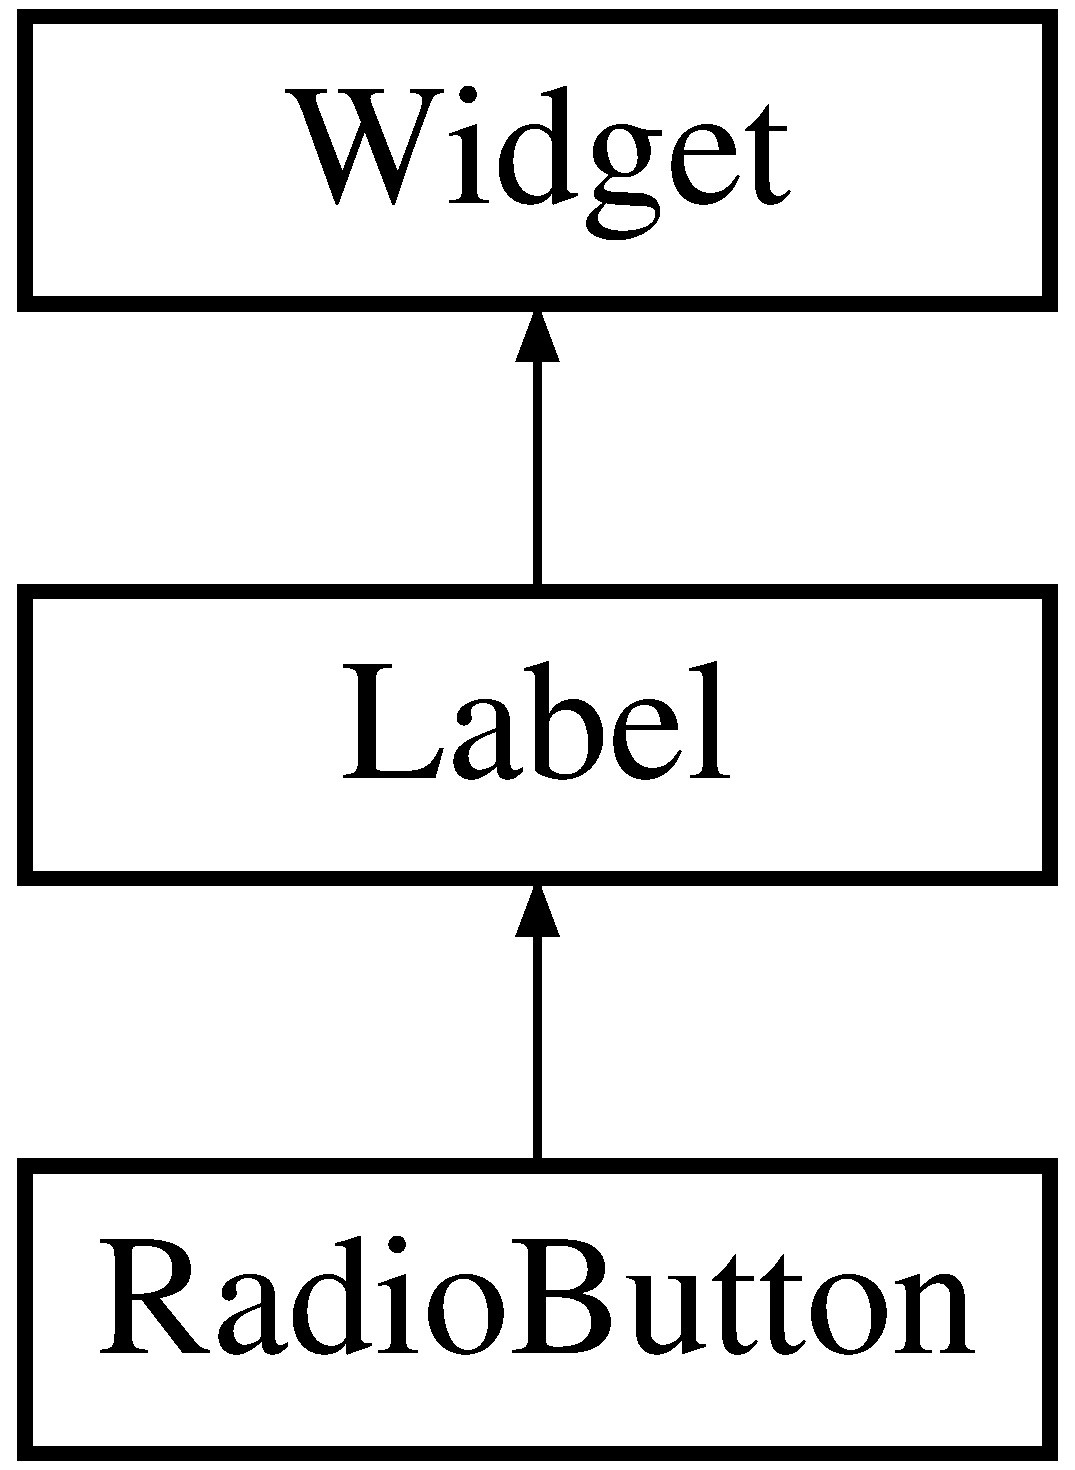
\includegraphics[height=3.000000cm]{class_radio_button}
\end{center}
\end{figure}
\subsection*{Publikus tagfüggvények}
\begin{DoxyCompactItemize}
\item 
\hyperlink{class_radio_button_af4fe7e144ad4ff848bcf4261a359c6e3}{Radio\+Button} (int x, int y, int button\+Size, std\+::string text, int value)
\begin{DoxyCompactList}\small\item\em Létrehoz egy új kiválasztó gombot. \end{DoxyCompactList}\item 
virtual void \hyperlink{class_radio_button_a296e30588da8a4767164c2dfc5d25a71}{Draw} ()
\begin{DoxyCompactList}\small\item\em Kirajzolja a gombot. \end{DoxyCompactList}\item 
virtual void \hyperlink{class_radio_button_a9287d026f57bdfedd878269ec4648135}{Handle} (\hyperlink{structgenv_1_1event}{genv\+::event} ev)
\begin{DoxyCompactList}\small\item\em Kezeli a widgetet az inputnak megfelelõen. \end{DoxyCompactList}\item 
virtual bool \hyperlink{class_radio_button_a94ab27ee37cdd639a185cb746ad7b32f}{Is\+In\+Line} (int x, int y)
\begin{DoxyCompactList}\small\item\em Megadja, hogy egy koordináta rajta van-\/e a widgeten. \end{DoxyCompactList}\item 
void \hyperlink{class_radio_button_a23ff4c296d56f8254b8bcb9afe4f5ee9}{Set\+Selection} (bool value)
\begin{DoxyCompactList}\small\item\em Beállítja, hogy ki van-\/e jelölve. \end{DoxyCompactList}\item 
bool \hyperlink{class_radio_button_a80163b8c471be945857d5a32e3a68056}{Get\+Selection} ()
\begin{DoxyCompactList}\small\item\em Megadja, hogy ki van-\/e jelölve. \end{DoxyCompactList}\item 
int \hyperlink{class_radio_button_a1961313659285fab02247085eb87ceee}{Get\+Value} ()
\begin{DoxyCompactList}\small\item\em Megadja a gomb értékét. \end{DoxyCompactList}\end{DoxyCompactItemize}
\subsection*{Privát tagfüggvények}
\begin{DoxyCompactItemize}
\item 
void \hyperlink{class_radio_button_afaf4b1617e725b65849d23c057dc3fa7}{Draw\+Circle} (int x, int y, int r, int thickness)
\begin{DoxyCompactList}\small\item\em Rajzol egy kört. \end{DoxyCompactList}\end{DoxyCompactItemize}
\subsection*{Privát attribútumok}
\begin{DoxyCompactItemize}
\item 
int \hyperlink{class_radio_button_a98ca476a4f3f93bdadd03c495b1457c9}{Value}
\item 
bool \hyperlink{class_radio_button_aa3ecd38f7d2f5a9b21d1b0ce9f36ecb0}{Is\+Selected}
\item 
\hyperlink{class_colour}{Colour} $\ast$ \hyperlink{class_radio_button_a944ef6b993774e3c36523915a2bb70bd}{on\+Click\+Colour}
\end{DoxyCompactItemize}
\subsection*{Additional Inherited Members}


\subsection{Konstruktorok és destruktorok dokumentációja}
\mbox{\Hypertarget{class_radio_button_af4fe7e144ad4ff848bcf4261a359c6e3}\label{class_radio_button_af4fe7e144ad4ff848bcf4261a359c6e3}} 
\index{Radio\+Button@{Radio\+Button}!Radio\+Button@{Radio\+Button}}
\index{Radio\+Button@{Radio\+Button}!Radio\+Button@{Radio\+Button}}
\subsubsection{\texorpdfstring{Radio\+Button()}{RadioButton()}}
{\footnotesize\ttfamily Radio\+Button\+::\+Radio\+Button (\begin{DoxyParamCaption}\item[{int}]{x,  }\item[{int}]{y,  }\item[{int}]{button\+Size,  }\item[{std\+::string}]{text,  }\item[{int}]{value }\end{DoxyParamCaption})}



Létrehoz egy új kiválasztó gombot. 


\begin{DoxyParams}{Paraméterek}
{\em x} & int Az x koordináta \\
\hline
{\em y} & int Az y koordináta \\
\hline
{\em button\+Size} & int A gomb sugara \\
\hline
{\em text} & std\+::string A gomb szövege \\
\hline
{\em value} & int A gomb értéke \\
\hline
\end{DoxyParams}


\subsection{Tagfüggvények dokumentációja}
\mbox{\Hypertarget{class_radio_button_a296e30588da8a4767164c2dfc5d25a71}\label{class_radio_button_a296e30588da8a4767164c2dfc5d25a71}} 
\index{Radio\+Button@{Radio\+Button}!Draw@{Draw}}
\index{Draw@{Draw}!Radio\+Button@{Radio\+Button}}
\subsubsection{\texorpdfstring{Draw()}{Draw()}}
{\footnotesize\ttfamily void Radio\+Button\+::\+Draw (\begin{DoxyParamCaption}{ }\end{DoxyParamCaption})\hspace{0.3cm}{\ttfamily [virtual]}}



Kirajzolja a gombot. 

\begin{DoxyReturn}{Visszatérési érték}
virtual void 
\end{DoxyReturn}


Újraimplementált ősök\+: \hyperlink{class_label_a184df028b3aa8c7f8dec8ecb90533319}{Label}.

\mbox{\Hypertarget{class_radio_button_afaf4b1617e725b65849d23c057dc3fa7}\label{class_radio_button_afaf4b1617e725b65849d23c057dc3fa7}} 
\index{Radio\+Button@{Radio\+Button}!Draw\+Circle@{Draw\+Circle}}
\index{Draw\+Circle@{Draw\+Circle}!Radio\+Button@{Radio\+Button}}
\subsubsection{\texorpdfstring{Draw\+Circle()}{DrawCircle()}}
{\footnotesize\ttfamily void Radio\+Button\+::\+Draw\+Circle (\begin{DoxyParamCaption}\item[{int}]{x,  }\item[{int}]{y,  }\item[{int}]{r,  }\item[{int}]{thickness }\end{DoxyParamCaption})\hspace{0.3cm}{\ttfamily [private]}}



Rajzol egy kört. 


\begin{DoxyParams}{Paraméterek}
{\em x} & int A kör középpontjának x koordinátája \\
\hline
{\em y} & int A kör középpontjának y koordinátája \\
\hline
{\em r} & int A kör sugara \\
\hline
{\em thickness} & int A kör vastagsága \\
\hline
\end{DoxyParams}
\begin{DoxyReturn}{Visszatérési érték}
void 
\end{DoxyReturn}
\mbox{\Hypertarget{class_radio_button_a80163b8c471be945857d5a32e3a68056}\label{class_radio_button_a80163b8c471be945857d5a32e3a68056}} 
\index{Radio\+Button@{Radio\+Button}!Get\+Selection@{Get\+Selection}}
\index{Get\+Selection@{Get\+Selection}!Radio\+Button@{Radio\+Button}}
\subsubsection{\texorpdfstring{Get\+Selection()}{GetSelection()}}
{\footnotesize\ttfamily bool Radio\+Button\+::\+Get\+Selection (\begin{DoxyParamCaption}{ }\end{DoxyParamCaption})}



Megadja, hogy ki van-\/e jelölve. 

\begin{DoxyReturn}{Visszatérési érték}
bool A kijelölés értéke 
\end{DoxyReturn}
\mbox{\Hypertarget{class_radio_button_a1961313659285fab02247085eb87ceee}\label{class_radio_button_a1961313659285fab02247085eb87ceee}} 
\index{Radio\+Button@{Radio\+Button}!Get\+Value@{Get\+Value}}
\index{Get\+Value@{Get\+Value}!Radio\+Button@{Radio\+Button}}
\subsubsection{\texorpdfstring{Get\+Value()}{GetValue()}}
{\footnotesize\ttfamily int Radio\+Button\+::\+Get\+Value (\begin{DoxyParamCaption}{ }\end{DoxyParamCaption})}



Megadja a gomb értékét. 

\begin{DoxyReturn}{Visszatérési érték}
int A gomb értéke 
\end{DoxyReturn}
\mbox{\Hypertarget{class_radio_button_a9287d026f57bdfedd878269ec4648135}\label{class_radio_button_a9287d026f57bdfedd878269ec4648135}} 
\index{Radio\+Button@{Radio\+Button}!Handle@{Handle}}
\index{Handle@{Handle}!Radio\+Button@{Radio\+Button}}
\subsubsection{\texorpdfstring{Handle()}{Handle()}}
{\footnotesize\ttfamily void Radio\+Button\+::\+Handle (\begin{DoxyParamCaption}\item[{\hyperlink{structgenv_1_1event}{genv\+::event}}]{ev }\end{DoxyParamCaption})\hspace{0.3cm}{\ttfamily [virtual]}}



Kezeli a widgetet az inputnak megfelelõen. 


\begin{DoxyParams}{Paraméterek}
{\em ev} & \hyperlink{structgenv_1_1event}{genv\+::event} Az input eventje \\
\hline
\end{DoxyParams}
\begin{DoxyReturn}{Visszatérési érték}
virtual void 
\end{DoxyReturn}


Újraimplementált ősök\+: \hyperlink{class_label_a5cf04da7def075453b5c0fda93a1b575}{Label}.

\mbox{\Hypertarget{class_radio_button_a94ab27ee37cdd639a185cb746ad7b32f}\label{class_radio_button_a94ab27ee37cdd639a185cb746ad7b32f}} 
\index{Radio\+Button@{Radio\+Button}!Is\+In\+Line@{Is\+In\+Line}}
\index{Is\+In\+Line@{Is\+In\+Line}!Radio\+Button@{Radio\+Button}}
\subsubsection{\texorpdfstring{Is\+In\+Line()}{IsInLine()}}
{\footnotesize\ttfamily bool Radio\+Button\+::\+Is\+In\+Line (\begin{DoxyParamCaption}\item[{int}]{x,  }\item[{int}]{y }\end{DoxyParamCaption})\hspace{0.3cm}{\ttfamily [virtual]}}



Megadja, hogy egy koordináta rajta van-\/e a widgeten. 


\begin{DoxyParams}{Paraméterek}
{\em x} & int Az x koordináta \\
\hline
{\em y} & int Az y koordináta \\
\hline
\end{DoxyParams}
\begin{DoxyReturn}{Visszatérési érték}
virtual bool 
\end{DoxyReturn}


Újraimplementált ősök\+: \hyperlink{class_label_a918ebb45dbaa5484643355cf5ab4be47}{Label}.

\mbox{\Hypertarget{class_radio_button_a23ff4c296d56f8254b8bcb9afe4f5ee9}\label{class_radio_button_a23ff4c296d56f8254b8bcb9afe4f5ee9}} 
\index{Radio\+Button@{Radio\+Button}!Set\+Selection@{Set\+Selection}}
\index{Set\+Selection@{Set\+Selection}!Radio\+Button@{Radio\+Button}}
\subsubsection{\texorpdfstring{Set\+Selection()}{SetSelection()}}
{\footnotesize\ttfamily void Radio\+Button\+::\+Set\+Selection (\begin{DoxyParamCaption}\item[{bool}]{value }\end{DoxyParamCaption})}



Beállítja, hogy ki van-\/e jelölve. 


\begin{DoxyParams}{Paraméterek}
{\em value} & bool A kijelölés értéke \\
\hline
\end{DoxyParams}
\begin{DoxyReturn}{Visszatérési érték}
void 
\end{DoxyReturn}


\subsection{Adattagok dokumentációja}
\mbox{\Hypertarget{class_radio_button_aa3ecd38f7d2f5a9b21d1b0ce9f36ecb0}\label{class_radio_button_aa3ecd38f7d2f5a9b21d1b0ce9f36ecb0}} 
\index{Radio\+Button@{Radio\+Button}!Is\+Selected@{Is\+Selected}}
\index{Is\+Selected@{Is\+Selected}!Radio\+Button@{Radio\+Button}}
\subsubsection{\texorpdfstring{Is\+Selected}{IsSelected}}
{\footnotesize\ttfamily bool Radio\+Button\+::\+Is\+Selected\hspace{0.3cm}{\ttfamily [private]}}

A gomb kiválasztottsága \mbox{\Hypertarget{class_radio_button_a944ef6b993774e3c36523915a2bb70bd}\label{class_radio_button_a944ef6b993774e3c36523915a2bb70bd}} 
\index{Radio\+Button@{Radio\+Button}!on\+Click\+Colour@{on\+Click\+Colour}}
\index{on\+Click\+Colour@{on\+Click\+Colour}!Radio\+Button@{Radio\+Button}}
\subsubsection{\texorpdfstring{on\+Click\+Colour}{onClickColour}}
{\footnotesize\ttfamily \hyperlink{class_colour}{Colour}$\ast$ Radio\+Button\+::on\+Click\+Colour\hspace{0.3cm}{\ttfamily [private]}}

A gomb színe kattintáskor \mbox{\Hypertarget{class_radio_button_a98ca476a4f3f93bdadd03c495b1457c9}\label{class_radio_button_a98ca476a4f3f93bdadd03c495b1457c9}} 
\index{Radio\+Button@{Radio\+Button}!Value@{Value}}
\index{Value@{Value}!Radio\+Button@{Radio\+Button}}
\subsubsection{\texorpdfstring{Value}{Value}}
{\footnotesize\ttfamily int Radio\+Button\+::\+Value\hspace{0.3cm}{\ttfamily [private]}}

A gomb értéke 

Ez a dokumentáció az osztályról a következő fájlok alapján készült\+:\begin{DoxyCompactItemize}
\item 
Radio\+Button.\+h\item 
Radio\+Button.\+cpp\end{DoxyCompactItemize}

\hypertarget{class_radio_button_holder}{}\section{Radio\+Button\+Holder osztályreferencia}
\label{class_radio_button_holder}\index{Radio\+Button\+Holder@{Radio\+Button\+Holder}}
A Radio\+Button\+Holder osztály származási diagramja\+:\begin{figure}[H]
\begin{center}
\leavevmode
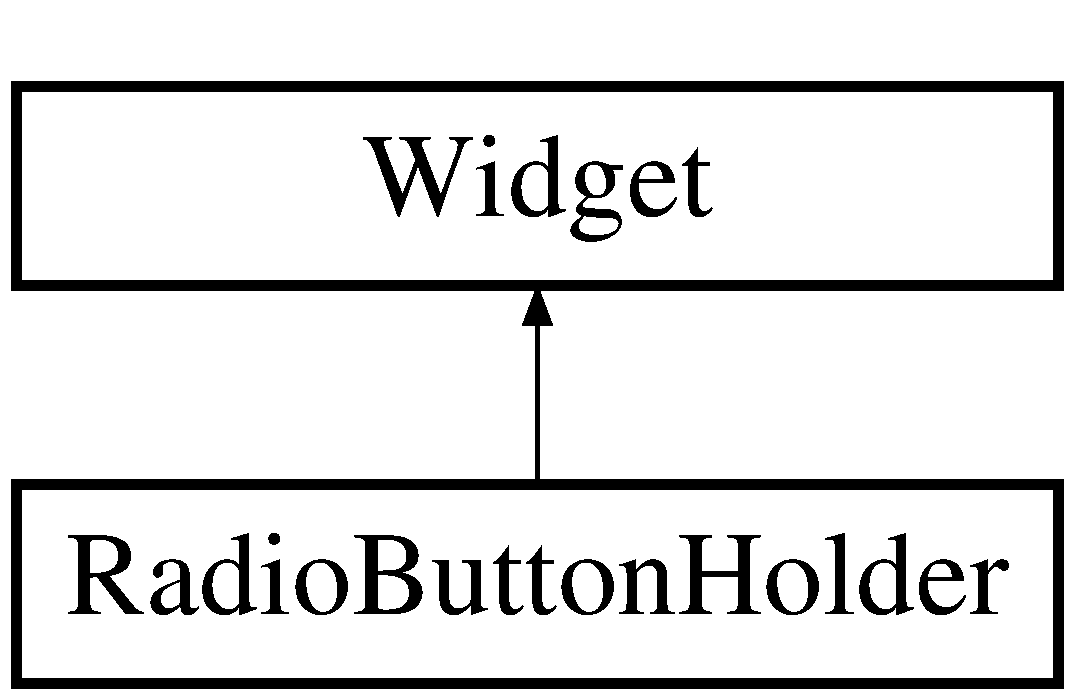
\includegraphics[height=2.000000cm]{class_radio_button_holder}
\end{center}
\end{figure}
\subsection*{Publikus tagfüggvények}
\begin{DoxyCompactItemize}
\item 
\hyperlink{class_radio_button_holder_ab100a3d26a036b76ead2bcd4331e8552}{Radio\+Button\+Holder} ()
\begin{DoxyCompactList}\small\item\em Létrehot egy kiválasztó gomb tartó objektumot. \end{DoxyCompactList}\item 
void \hyperlink{class_radio_button_holder_ab9ac730a7440439eb73b892f193741ae}{Add\+Radio\+Button} (\hyperlink{class_radio_button}{Radio\+Button} $\ast$button)
\begin{DoxyCompactList}\small\item\em A listához ad egy új gombot. \end{DoxyCompactList}\item 
void \hyperlink{class_radio_button_holder_a217e5620f70f0d2633e70896ad166f70}{Remove\+Radio\+Button} (\hyperlink{class_radio_button}{Radio\+Button} $\ast$button)
\begin{DoxyCompactList}\small\item\em Eltávolít egy gombot. \end{DoxyCompactList}\item 
void \hyperlink{class_radio_button_holder_a8a44f58d480a8c1b4822adb9e9df0c98}{Remove\+Radio\+Button} (int place)
\begin{DoxyCompactList}\small\item\em Eltávolít egy gombot. \end{DoxyCompactList}\item 
int \hyperlink{class_radio_button_holder_ad185ab84d978e645eac54f236069705b}{Get\+Currently\+Selected} ()
\begin{DoxyCompactList}\small\item\em Megadja a jelenleg kiválasztott gomb sorszámát. \end{DoxyCompactList}\item 
int \hyperlink{class_radio_button_holder_a5ed73396ddd57f3de474a7487429bae3}{Currently\+Selected\+Value} ()
\begin{DoxyCompactList}\small\item\em Megadja a jelenleg kiválasztott gomb értékét. \end{DoxyCompactList}\item 
void \hyperlink{class_radio_button_holder_a1b15e73021c8e2022d43b12f4246182d}{Set\+Event\+Void} (std\+::function$<$ void(\hyperlink{class_radio_button_holder}{Radio\+Button\+Holder} $\ast$)$>$ event)
\begin{DoxyCompactList}\small\item\em Egy gomra történő kattintáskor meghívandó esemény. \end{DoxyCompactList}\item 
virtual void \hyperlink{class_radio_button_holder_a70d6ba1724bdb68afe351d0474cbd767}{Draw} ()
\begin{DoxyCompactList}\small\item\em Kirajzolja a widgeteket. \end{DoxyCompactList}\item 
virtual void \hyperlink{class_radio_button_holder_a7b4ed9e75eef252ad20c3cbcb8547981}{Handle} (\hyperlink{structgenv_1_1event}{genv\+::event} ev)
\begin{DoxyCompactList}\small\item\em Kezeli a widgeteket az inputnak megfelelõen. \end{DoxyCompactList}\item 
virtual bool \hyperlink{class_radio_button_holder_aa6d6fe7d9eb9ce9c2628f432ef129e01}{Is\+In\+Line} (int x, int y)
\begin{DoxyCompactList}\small\item\em Megadja, hogy egy koordináta rajta van-\/e a widgeten. \end{DoxyCompactList}\end{DoxyCompactItemize}
\subsection*{Privát tagfüggvények}
\begin{DoxyCompactItemize}
\item 
void \hyperlink{class_radio_button_holder_aeca94b584cd2a969f38f587f08ff43df}{Check\+Null} ()
\begin{DoxyCompactList}\small\item\em Ellenőrzi, hogy vannak-\/e gombok. \end{DoxyCompactList}\end{DoxyCompactItemize}
\subsection*{Privát attribútumok}
\begin{DoxyCompactItemize}
\item 
std\+::vector$<$ \hyperlink{class_radio_button}{Radio\+Button} $\ast$ $>$ \hyperlink{class_radio_button_holder_aaed6e22df55ff0174b150c675caff07a}{radio\+Buttons}
\item 
std\+::function$<$ void(\hyperlink{class_radio_button_holder}{Radio\+Button\+Holder} $\ast$)$>$ \hyperlink{class_radio_button_holder_ac2ecfd4a57032afaa6455f9b559a00b3}{On\+Event}
\item 
int \hyperlink{class_radio_button_holder_a115a7d96d3c3a7a97d3e9bc4d04b50e0}{Button\+Count}
\item 
int \hyperlink{class_radio_button_holder_a72c73d2f99d20384f334903cec24040e}{Currently\+Selected}
\end{DoxyCompactItemize}
\subsection*{Additional Inherited Members}


\subsection{Konstruktorok és destruktorok dokumentációja}
\mbox{\Hypertarget{class_radio_button_holder_ab100a3d26a036b76ead2bcd4331e8552}\label{class_radio_button_holder_ab100a3d26a036b76ead2bcd4331e8552}} 
\index{Radio\+Button\+Holder@{Radio\+Button\+Holder}!Radio\+Button\+Holder@{Radio\+Button\+Holder}}
\index{Radio\+Button\+Holder@{Radio\+Button\+Holder}!Radio\+Button\+Holder@{Radio\+Button\+Holder}}
\subsubsection{\texorpdfstring{Radio\+Button\+Holder()}{RadioButtonHolder()}}
{\footnotesize\ttfamily Radio\+Button\+Holder\+::\+Radio\+Button\+Holder (\begin{DoxyParamCaption}{ }\end{DoxyParamCaption})}



Létrehot egy kiválasztó gomb tartó objektumot. 



\subsection{Tagfüggvények dokumentációja}
\mbox{\Hypertarget{class_radio_button_holder_ab9ac730a7440439eb73b892f193741ae}\label{class_radio_button_holder_ab9ac730a7440439eb73b892f193741ae}} 
\index{Radio\+Button\+Holder@{Radio\+Button\+Holder}!Add\+Radio\+Button@{Add\+Radio\+Button}}
\index{Add\+Radio\+Button@{Add\+Radio\+Button}!Radio\+Button\+Holder@{Radio\+Button\+Holder}}
\subsubsection{\texorpdfstring{Add\+Radio\+Button()}{AddRadioButton()}}
{\footnotesize\ttfamily void Radio\+Button\+Holder\+::\+Add\+Radio\+Button (\begin{DoxyParamCaption}\item[{\hyperlink{class_radio_button}{Radio\+Button} $\ast$}]{button }\end{DoxyParamCaption})}



A listához ad egy új gombot. 


\begin{DoxyParams}{Paraméterek}
{\em button} & Radio\+Button$\ast$ Az új gomn \\
\hline
\end{DoxyParams}
\begin{DoxyReturn}{Visszatérési érték}
void 
\end{DoxyReturn}
\mbox{\Hypertarget{class_radio_button_holder_aeca94b584cd2a969f38f587f08ff43df}\label{class_radio_button_holder_aeca94b584cd2a969f38f587f08ff43df}} 
\index{Radio\+Button\+Holder@{Radio\+Button\+Holder}!Check\+Null@{Check\+Null}}
\index{Check\+Null@{Check\+Null}!Radio\+Button\+Holder@{Radio\+Button\+Holder}}
\subsubsection{\texorpdfstring{Check\+Null()}{CheckNull()}}
{\footnotesize\ttfamily void Radio\+Button\+Holder\+::\+Check\+Null (\begin{DoxyParamCaption}{ }\end{DoxyParamCaption})\hspace{0.3cm}{\ttfamily [private]}}



Ellenőrzi, hogy vannak-\/e gombok. 

\begin{DoxyReturn}{Visszatérési érték}
void 
\end{DoxyReturn}
\mbox{\Hypertarget{class_radio_button_holder_a5ed73396ddd57f3de474a7487429bae3}\label{class_radio_button_holder_a5ed73396ddd57f3de474a7487429bae3}} 
\index{Radio\+Button\+Holder@{Radio\+Button\+Holder}!Currently\+Selected\+Value@{Currently\+Selected\+Value}}
\index{Currently\+Selected\+Value@{Currently\+Selected\+Value}!Radio\+Button\+Holder@{Radio\+Button\+Holder}}
\subsubsection{\texorpdfstring{Currently\+Selected\+Value()}{CurrentlySelectedValue()}}
{\footnotesize\ttfamily int Radio\+Button\+Holder\+::\+Currently\+Selected\+Value (\begin{DoxyParamCaption}{ }\end{DoxyParamCaption})}



Megadja a jelenleg kiválasztott gomb értékét. 

\begin{DoxyReturn}{Visszatérési érték}
int A jelenleg kiválasztott gomb értéke 
\end{DoxyReturn}
\mbox{\Hypertarget{class_radio_button_holder_a70d6ba1724bdb68afe351d0474cbd767}\label{class_radio_button_holder_a70d6ba1724bdb68afe351d0474cbd767}} 
\index{Radio\+Button\+Holder@{Radio\+Button\+Holder}!Draw@{Draw}}
\index{Draw@{Draw}!Radio\+Button\+Holder@{Radio\+Button\+Holder}}
\subsubsection{\texorpdfstring{Draw()}{Draw()}}
{\footnotesize\ttfamily void Radio\+Button\+Holder\+::\+Draw (\begin{DoxyParamCaption}{ }\end{DoxyParamCaption})\hspace{0.3cm}{\ttfamily [virtual]}}



Kirajzolja a widgeteket. 

\begin{DoxyReturn}{Visszatérési érték}
virtual void 
\end{DoxyReturn}


Megvalósítja a következőket\+: \hyperlink{class_widget_ac4c2063cd671468ad05d84cfe963c032}{Widget}.

\mbox{\Hypertarget{class_radio_button_holder_ad185ab84d978e645eac54f236069705b}\label{class_radio_button_holder_ad185ab84d978e645eac54f236069705b}} 
\index{Radio\+Button\+Holder@{Radio\+Button\+Holder}!Get\+Currently\+Selected@{Get\+Currently\+Selected}}
\index{Get\+Currently\+Selected@{Get\+Currently\+Selected}!Radio\+Button\+Holder@{Radio\+Button\+Holder}}
\subsubsection{\texorpdfstring{Get\+Currently\+Selected()}{GetCurrentlySelected()}}
{\footnotesize\ttfamily int Radio\+Button\+Holder\+::\+Get\+Currently\+Selected (\begin{DoxyParamCaption}{ }\end{DoxyParamCaption})}



Megadja a jelenleg kiválasztott gomb sorszámát. 

\begin{DoxyReturn}{Visszatérési érték}
int A jelenleg kiválasztott gomb sorszáma 
\end{DoxyReturn}
\mbox{\Hypertarget{class_radio_button_holder_a7b4ed9e75eef252ad20c3cbcb8547981}\label{class_radio_button_holder_a7b4ed9e75eef252ad20c3cbcb8547981}} 
\index{Radio\+Button\+Holder@{Radio\+Button\+Holder}!Handle@{Handle}}
\index{Handle@{Handle}!Radio\+Button\+Holder@{Radio\+Button\+Holder}}
\subsubsection{\texorpdfstring{Handle()}{Handle()}}
{\footnotesize\ttfamily void Radio\+Button\+Holder\+::\+Handle (\begin{DoxyParamCaption}\item[{\hyperlink{structgenv_1_1event}{genv\+::event}}]{ev }\end{DoxyParamCaption})\hspace{0.3cm}{\ttfamily [virtual]}}



Kezeli a widgeteket az inputnak megfelelõen. 


\begin{DoxyParams}{Paraméterek}
{\em ev} & \hyperlink{structgenv_1_1event}{genv\+::event} Az input eventje \\
\hline
\end{DoxyParams}
\begin{DoxyReturn}{Visszatérési érték}
virtual void 
\end{DoxyReturn}


Megvalósítja a következőket\+: \hyperlink{class_widget_abf512e4606c7a5d44245a9b0246634a0}{Widget}.

\mbox{\Hypertarget{class_radio_button_holder_aa6d6fe7d9eb9ce9c2628f432ef129e01}\label{class_radio_button_holder_aa6d6fe7d9eb9ce9c2628f432ef129e01}} 
\index{Radio\+Button\+Holder@{Radio\+Button\+Holder}!Is\+In\+Line@{Is\+In\+Line}}
\index{Is\+In\+Line@{Is\+In\+Line}!Radio\+Button\+Holder@{Radio\+Button\+Holder}}
\subsubsection{\texorpdfstring{Is\+In\+Line()}{IsInLine()}}
{\footnotesize\ttfamily bool Radio\+Button\+Holder\+::\+Is\+In\+Line (\begin{DoxyParamCaption}\item[{int}]{x,  }\item[{int}]{y }\end{DoxyParamCaption})\hspace{0.3cm}{\ttfamily [virtual]}}



Megadja, hogy egy koordináta rajta van-\/e a widgeten. 


\begin{DoxyParams}{Paraméterek}
{\em x} & int Az x koordináta \\
\hline
{\em y} & int Az y koordináta \\
\hline
\end{DoxyParams}
\begin{DoxyReturn}{Visszatérési érték}
virtual bool 
\end{DoxyReturn}


Megvalósítja a következőket\+: \hyperlink{class_widget_a7a18323ef481add82e5edba5c0c6ec06}{Widget}.

\mbox{\Hypertarget{class_radio_button_holder_a217e5620f70f0d2633e70896ad166f70}\label{class_radio_button_holder_a217e5620f70f0d2633e70896ad166f70}} 
\index{Radio\+Button\+Holder@{Radio\+Button\+Holder}!Remove\+Radio\+Button@{Remove\+Radio\+Button}}
\index{Remove\+Radio\+Button@{Remove\+Radio\+Button}!Radio\+Button\+Holder@{Radio\+Button\+Holder}}
\subsubsection{\texorpdfstring{Remove\+Radio\+Button()}{RemoveRadioButton()}\hspace{0.1cm}{\footnotesize\ttfamily [1/2]}}
{\footnotesize\ttfamily void Radio\+Button\+Holder\+::\+Remove\+Radio\+Button (\begin{DoxyParamCaption}\item[{\hyperlink{class_radio_button}{Radio\+Button} $\ast$}]{button }\end{DoxyParamCaption})}



Eltávolít egy gombot. 


\begin{DoxyParams}{Paraméterek}
{\em button} & Radio\+Button$\ast$ Az eltávolítandó gomb \\
\hline
\end{DoxyParams}
\begin{DoxyReturn}{Visszatérési érték}
void 
\end{DoxyReturn}
\mbox{\Hypertarget{class_radio_button_holder_a8a44f58d480a8c1b4822adb9e9df0c98}\label{class_radio_button_holder_a8a44f58d480a8c1b4822adb9e9df0c98}} 
\index{Radio\+Button\+Holder@{Radio\+Button\+Holder}!Remove\+Radio\+Button@{Remove\+Radio\+Button}}
\index{Remove\+Radio\+Button@{Remove\+Radio\+Button}!Radio\+Button\+Holder@{Radio\+Button\+Holder}}
\subsubsection{\texorpdfstring{Remove\+Radio\+Button()}{RemoveRadioButton()}\hspace{0.1cm}{\footnotesize\ttfamily [2/2]}}
{\footnotesize\ttfamily void Radio\+Button\+Holder\+::\+Remove\+Radio\+Button (\begin{DoxyParamCaption}\item[{int}]{place }\end{DoxyParamCaption})}



Eltávolít egy gombot. 


\begin{DoxyParams}{Paraméterek}
{\em place} & int Az eltávolítandó gomb sorszáma \\
\hline
\end{DoxyParams}
\begin{DoxyReturn}{Visszatérési érték}
void 
\end{DoxyReturn}
\mbox{\Hypertarget{class_radio_button_holder_a1b15e73021c8e2022d43b12f4246182d}\label{class_radio_button_holder_a1b15e73021c8e2022d43b12f4246182d}} 
\index{Radio\+Button\+Holder@{Radio\+Button\+Holder}!Set\+Event\+Void@{Set\+Event\+Void}}
\index{Set\+Event\+Void@{Set\+Event\+Void}!Radio\+Button\+Holder@{Radio\+Button\+Holder}}
\subsubsection{\texorpdfstring{Set\+Event\+Void()}{SetEventVoid()}}
{\footnotesize\ttfamily void Radio\+Button\+Holder\+::\+Set\+Event\+Void (\begin{DoxyParamCaption}\item[{std\+::function$<$ void(\hyperlink{class_radio_button_holder}{Radio\+Button\+Holder} $\ast$)$>$}]{event }\end{DoxyParamCaption})}



Egy gomra történő kattintáskor meghívandó esemény. 


\begin{DoxyParams}{Paraméterek}
{\em Radio\+Button\+Holder$\ast$} & A meghívandó esemény \\
\hline
\end{DoxyParams}
\begin{DoxyReturn}{Visszatérési érték}
void 
\end{DoxyReturn}


\subsection{Adattagok dokumentációja}
\mbox{\Hypertarget{class_radio_button_holder_a115a7d96d3c3a7a97d3e9bc4d04b50e0}\label{class_radio_button_holder_a115a7d96d3c3a7a97d3e9bc4d04b50e0}} 
\index{Radio\+Button\+Holder@{Radio\+Button\+Holder}!Button\+Count@{Button\+Count}}
\index{Button\+Count@{Button\+Count}!Radio\+Button\+Holder@{Radio\+Button\+Holder}}
\subsubsection{\texorpdfstring{Button\+Count}{ButtonCount}}
{\footnotesize\ttfamily int Radio\+Button\+Holder\+::\+Button\+Count\hspace{0.3cm}{\ttfamily [private]}}

A gombok száma \mbox{\Hypertarget{class_radio_button_holder_a72c73d2f99d20384f334903cec24040e}\label{class_radio_button_holder_a72c73d2f99d20384f334903cec24040e}} 
\index{Radio\+Button\+Holder@{Radio\+Button\+Holder}!Currently\+Selected@{Currently\+Selected}}
\index{Currently\+Selected@{Currently\+Selected}!Radio\+Button\+Holder@{Radio\+Button\+Holder}}
\subsubsection{\texorpdfstring{Currently\+Selected}{CurrentlySelected}}
{\footnotesize\ttfamily int Radio\+Button\+Holder\+::\+Currently\+Selected\hspace{0.3cm}{\ttfamily [private]}}

A jeleneg kiválasztott gomb sorszáma \mbox{\Hypertarget{class_radio_button_holder_ac2ecfd4a57032afaa6455f9b559a00b3}\label{class_radio_button_holder_ac2ecfd4a57032afaa6455f9b559a00b3}} 
\index{Radio\+Button\+Holder@{Radio\+Button\+Holder}!On\+Event@{On\+Event}}
\index{On\+Event@{On\+Event}!Radio\+Button\+Holder@{Radio\+Button\+Holder}}
\subsubsection{\texorpdfstring{On\+Event}{OnEvent}}
{\footnotesize\ttfamily std\+::function$<$void(\hyperlink{class_radio_button_holder}{Radio\+Button\+Holder}$\ast$)$>$ Radio\+Button\+Holder\+::\+On\+Event\hspace{0.3cm}{\ttfamily [private]}}

A meghíndó esemény \mbox{\Hypertarget{class_radio_button_holder_aaed6e22df55ff0174b150c675caff07a}\label{class_radio_button_holder_aaed6e22df55ff0174b150c675caff07a}} 
\index{Radio\+Button\+Holder@{Radio\+Button\+Holder}!radio\+Buttons@{radio\+Buttons}}
\index{radio\+Buttons@{radio\+Buttons}!Radio\+Button\+Holder@{Radio\+Button\+Holder}}
\subsubsection{\texorpdfstring{radio\+Buttons}{radioButtons}}
{\footnotesize\ttfamily std\+::vector$<$\hyperlink{class_radio_button}{Radio\+Button}$\ast$$>$ Radio\+Button\+Holder\+::radio\+Buttons\hspace{0.3cm}{\ttfamily [private]}}

A tárolt gombok listája 

Ez a dokumentáció az osztályról a következő fájlok alapján készült\+:\begin{DoxyCompactItemize}
\item 
Radio\+Button\+Holder.\+h\item 
Radio\+Button\+Holder.\+cpp\end{DoxyCompactItemize}

\hypertarget{class_selection_box}{}\section{Selection\+Box osztályreferencia}
\label{class_selection_box}\index{Selection\+Box@{Selection\+Box}}
A Selection\+Box osztály származási diagramja\+:\begin{figure}[H]
\begin{center}
\leavevmode
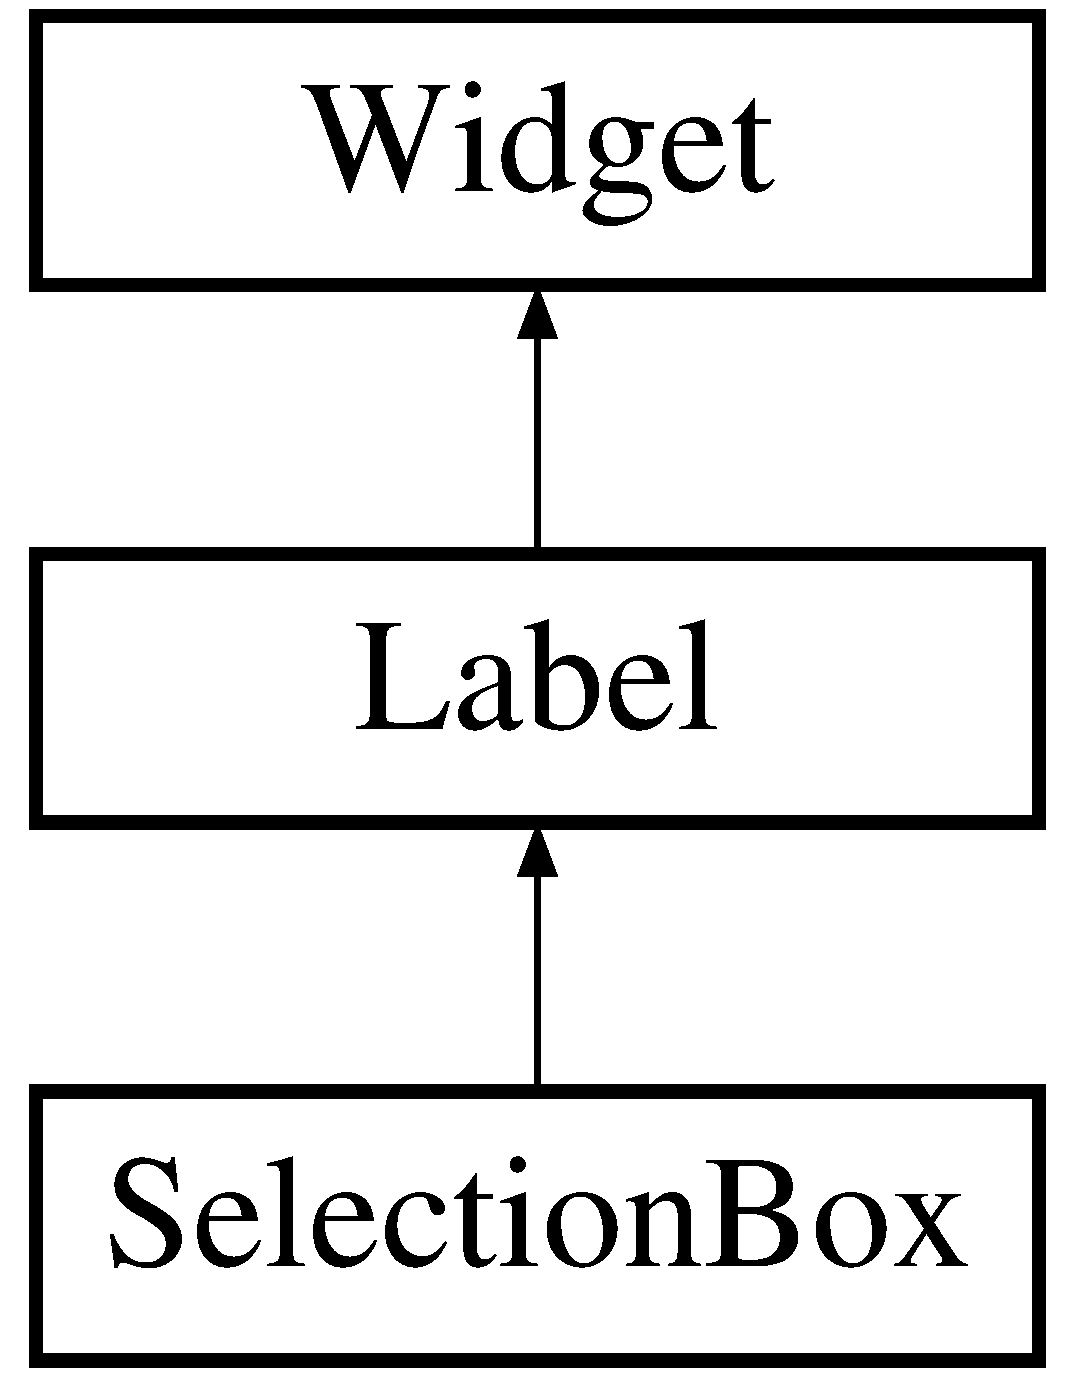
\includegraphics[height=3.000000cm]{class_selection_box}
\end{center}
\end{figure}
\subsection*{Publikus tagfüggvények}
\begin{DoxyCompactItemize}
\item 
\hyperlink{class_selection_box_a1d5613b94e9d7c57a12fedc783813f62}{Selection\+Box} (int x, int y, int x\+Size, int y\+Size, std\+::vector$<$ std\+::string $>$ values)
\item 
void \hyperlink{class_selection_box_a1c0b7b6c851180450964a4df0c7c15e8}{Draw} ()
\item 
void \hyperlink{class_selection_box_a4762480ce86018d74c0cfa271c9cce11}{Handle} (\hyperlink{structgenv_1_1event}{genv\+::event} ev)
\item 
bool \hyperlink{class_selection_box_a0378e1ec035f90dd04efac5d6a2c7132}{Is\+In\+Line} (int x, int y)
\item 
void \hyperlink{class_selection_box_a5f53112258e5b32ac9e0232c75a62eda}{Add\+Item} (std\+::string value)
\item 
void \hyperlink{class_selection_box_ae4bb0013ac37a323c72a426de84c08c8}{Remove\+Item} (std\+::string value)
\item 
void \hyperlink{class_selection_box_af81528e021ed52fee388cb6dea786446}{Remove\+Item} (int place)
\item 
int \hyperlink{class_selection_box_a11dadb7f3ebc3bc797f6747312c18597}{Currently\+Selected\+Value} ()
\item 
std\+::string \hyperlink{class_selection_box_a7bec61ef09f9198f93f88121074753ac}{Currently\+Selected\+Item} ()
\item 
void \hyperlink{class_selection_box_abd6e227d728b5802353d69c210997619}{Edit\+Selected\+Font\+Colour} (int r, int g, int b)
\item 
void \hyperlink{class_selection_box_aaa47aeeda9cb1d50e5c519f5a1bb9dab}{Edit\+Selected\+Front\+Colour} (int r, int g, int b)
\item 
void \hyperlink{class_selection_box_a572b7322795b52447cf6ed292e13e832}{Set\+Button\+Size} (int button)
\item 
void \hyperlink{class_selection_box_a4596a4d2ff08593fda4f1ddd1cfc6eea}{Edit\+Max\+Item\+In\+View} (int elements)
\end{DoxyCompactItemize}
\subsection*{Privát attribútumok}
\begin{DoxyCompactItemize}
\item 
bool \hyperlink{class_selection_box_ad7340177b4fc04b45cc26973f72002ac}{is\+Opened}
\item 
int \hyperlink{class_selection_box_a6a0fac038c98be9bdc85d4208ea5d1d5}{max\+Items\+In\+View}
\item 
int \hyperlink{class_selection_box_a5ecda83cc02b9aa23a1119b599c14420}{currently\+Selected}
\item 
int \hyperlink{class_selection_box_af7d6ac5ec9c1bec8093c4658c8d7eb4a}{mouse\+On\+Item}
\item 
int \hyperlink{class_selection_box_afcfc7749e3ec40e69d58f2774d32805b}{top\+Item}
\item 
\hyperlink{class_colour}{Colour} $\ast$ \hyperlink{class_selection_box_a6db5b172a719f48db281e6bd12e20d5e}{selected\+Font\+Colour}
\item 
\hyperlink{class_colour}{Colour} $\ast$ \hyperlink{class_selection_box_a3e20a7106c555781d74772c0dd983e9d}{selected\+Front\+Colour}
\item 
\hyperlink{class_colour}{Colour} $\ast$ \hyperlink{class_selection_box_a8f00181c55398686633e05055fe9050b}{button\+Colour}
\item 
\hyperlink{class_colour}{Colour} $\ast$ \hyperlink{class_selection_box_a671415d9b6a3625fcffdc0f8a2882f3a}{button\+On\+Click\+Colour}
\item 
int \hyperlink{class_selection_box_a91fe3df437f4ffe0e5885e9362c76e55}{button\+Size} = 15
\item 
std\+::vector$<$ std\+::string $>$ \hyperlink{class_selection_box_a8bac4f40a469f4ed3acba73a3e233390}{Values}
\end{DoxyCompactItemize}
\subsection*{Additional Inherited Members}


\subsection{Konstruktorok és destruktorok dokumentációja}
\mbox{\Hypertarget{class_selection_box_a1d5613b94e9d7c57a12fedc783813f62}\label{class_selection_box_a1d5613b94e9d7c57a12fedc783813f62}} 
\index{Selection\+Box@{Selection\+Box}!Selection\+Box@{Selection\+Box}}
\index{Selection\+Box@{Selection\+Box}!Selection\+Box@{Selection\+Box}}
\subsubsection{\texorpdfstring{Selection\+Box()}{SelectionBox()}}
{\footnotesize\ttfamily Selection\+Box\+::\+Selection\+Box (\begin{DoxyParamCaption}\item[{int}]{x,  }\item[{int}]{y,  }\item[{int}]{x\+Size,  }\item[{int}]{y\+Size,  }\item[{std\+::vector$<$ std\+::string $>$}]{values }\end{DoxyParamCaption})}

Egy leg�rd�l� men�t ad meg. 
\begin{DoxyParams}{Paraméterek}
{\em x} & A widget X poz�ci�ja \\
\hline
{\em y} & A widget Y poz�ci�ja \\
\hline
{\em x\+Size} & A widget hossza \\
\hline
{\em y\+Size} & A widget magass�ga \\
\hline
{\em values} & A widget kezd� �rt�keit tartalmazza \\
\hline
\end{DoxyParams}


\subsection{Tagfüggvények dokumentációja}
\mbox{\Hypertarget{class_selection_box_a5f53112258e5b32ac9e0232c75a62eda}\label{class_selection_box_a5f53112258e5b32ac9e0232c75a62eda}} 
\index{Selection\+Box@{Selection\+Box}!Add\+Item@{Add\+Item}}
\index{Add\+Item@{Add\+Item}!Selection\+Box@{Selection\+Box}}
\subsubsection{\texorpdfstring{Add\+Item()}{AddItem()}}
{\footnotesize\ttfamily void Selection\+Box\+::\+Add\+Item (\begin{DoxyParamCaption}\item[{std\+::string}]{value }\end{DoxyParamCaption})}

�j elemet ad hozz� a list�hoz 
\begin{DoxyParams}{Paraméterek}
{\em value} & Az �j elem \\
\hline
\end{DoxyParams}
\mbox{\Hypertarget{class_selection_box_a7bec61ef09f9198f93f88121074753ac}\label{class_selection_box_a7bec61ef09f9198f93f88121074753ac}} 
\index{Selection\+Box@{Selection\+Box}!Currently\+Selected\+Item@{Currently\+Selected\+Item}}
\index{Currently\+Selected\+Item@{Currently\+Selected\+Item}!Selection\+Box@{Selection\+Box}}
\subsubsection{\texorpdfstring{Currently\+Selected\+Item()}{CurrentlySelectedItem()}}
{\footnotesize\ttfamily std\+::string Selection\+Box\+::\+Currently\+Selected\+Item (\begin{DoxyParamCaption}{ }\end{DoxyParamCaption})}

Megadja a jelenleg kijel�lt elemet \begin{DoxyReturn}{Visszatérési érték}
A kijel�lt elem �rt�ke 
\end{DoxyReturn}
\mbox{\Hypertarget{class_selection_box_a11dadb7f3ebc3bc797f6747312c18597}\label{class_selection_box_a11dadb7f3ebc3bc797f6747312c18597}} 
\index{Selection\+Box@{Selection\+Box}!Currently\+Selected\+Value@{Currently\+Selected\+Value}}
\index{Currently\+Selected\+Value@{Currently\+Selected\+Value}!Selection\+Box@{Selection\+Box}}
\subsubsection{\texorpdfstring{Currently\+Selected\+Value()}{CurrentlySelectedValue()}}
{\footnotesize\ttfamily int Selection\+Box\+::\+Currently\+Selected\+Value (\begin{DoxyParamCaption}{ }\end{DoxyParamCaption})}

Megadja a jelenleg kijel�lt elem sorsz�m�t a list�ban \begin{DoxyReturn}{Visszatérési érték}
A kijel�lt elem sorsz�ma 
\end{DoxyReturn}
\mbox{\Hypertarget{class_selection_box_a1c0b7b6c851180450964a4df0c7c15e8}\label{class_selection_box_a1c0b7b6c851180450964a4df0c7c15e8}} 
\index{Selection\+Box@{Selection\+Box}!Draw@{Draw}}
\index{Draw@{Draw}!Selection\+Box@{Selection\+Box}}
\subsubsection{\texorpdfstring{Draw()}{Draw()}}
{\footnotesize\ttfamily void Selection\+Box\+::\+Draw (\begin{DoxyParamCaption}{ }\end{DoxyParamCaption})\hspace{0.3cm}{\ttfamily [virtual]}}

Ez felel a widget kirajzol�s��rt 

Újraimplementált ősök\+: \hyperlink{class_label_a184df028b3aa8c7f8dec8ecb90533319}{Label}.

\mbox{\Hypertarget{class_selection_box_a4596a4d2ff08593fda4f1ddd1cfc6eea}\label{class_selection_box_a4596a4d2ff08593fda4f1ddd1cfc6eea}} 
\index{Selection\+Box@{Selection\+Box}!Edit\+Max\+Item\+In\+View@{Edit\+Max\+Item\+In\+View}}
\index{Edit\+Max\+Item\+In\+View@{Edit\+Max\+Item\+In\+View}!Selection\+Box@{Selection\+Box}}
\subsubsection{\texorpdfstring{Edit\+Max\+Item\+In\+View()}{EditMaxItemInView()}}
{\footnotesize\ttfamily void Selection\+Box\+::\+Edit\+Max\+Item\+In\+View (\begin{DoxyParamCaption}\item[{int}]{elements }\end{DoxyParamCaption})}

�t�l�tja, hogy maximum h�ny elem l�tsz�djon a leny�l� men�ben. Amennyiben t�bb elemet tartalmaz, mint ez a sz�m, g�rgetni kell 
\begin{DoxyParams}{Paraméterek}
{\em Az} & egyszerre l�that� elemek sz�ma \\
\hline
\end{DoxyParams}
\mbox{\Hypertarget{class_selection_box_abd6e227d728b5802353d69c210997619}\label{class_selection_box_abd6e227d728b5802353d69c210997619}} 
\index{Selection\+Box@{Selection\+Box}!Edit\+Selected\+Font\+Colour@{Edit\+Selected\+Font\+Colour}}
\index{Edit\+Selected\+Font\+Colour@{Edit\+Selected\+Font\+Colour}!Selection\+Box@{Selection\+Box}}
\subsubsection{\texorpdfstring{Edit\+Selected\+Font\+Colour()}{EditSelectedFontColour()}}
{\footnotesize\ttfamily void Selection\+Box\+::\+Edit\+Selected\+Font\+Colour (\begin{DoxyParamCaption}\item[{int}]{r,  }\item[{int}]{g,  }\item[{int}]{b }\end{DoxyParamCaption})}

�t�l�tja kijel�lt sz�veg sz�n�t 
\begin{DoxyParams}{Paraméterek}
{\em r} & Az �j piros �rt�k \\
\hline
{\em g} & Az �j z�ld �rt�k \\
\hline
{\em b} & Az �j k�k �rt�k \\
\hline
\end{DoxyParams}
\mbox{\Hypertarget{class_selection_box_aaa47aeeda9cb1d50e5c519f5a1bb9dab}\label{class_selection_box_aaa47aeeda9cb1d50e5c519f5a1bb9dab}} 
\index{Selection\+Box@{Selection\+Box}!Edit\+Selected\+Front\+Colour@{Edit\+Selected\+Front\+Colour}}
\index{Edit\+Selected\+Front\+Colour@{Edit\+Selected\+Front\+Colour}!Selection\+Box@{Selection\+Box}}
\subsubsection{\texorpdfstring{Edit\+Selected\+Front\+Colour()}{EditSelectedFrontColour()}}
{\footnotesize\ttfamily void Selection\+Box\+::\+Edit\+Selected\+Front\+Colour (\begin{DoxyParamCaption}\item[{int}]{r,  }\item[{int}]{g,  }\item[{int}]{b }\end{DoxyParamCaption})}

�t�l�tja a kijel�lt el�t�r sz�n�t 
\begin{DoxyParams}{Paraméterek}
{\em r} & Az �j piros �rt�k \\
\hline
{\em g} & Az �j z�ld �rt�k \\
\hline
{\em b} & Az �j k�k �rt�k \\
\hline
\end{DoxyParams}
\mbox{\Hypertarget{class_selection_box_a4762480ce86018d74c0cfa271c9cce11}\label{class_selection_box_a4762480ce86018d74c0cfa271c9cce11}} 
\index{Selection\+Box@{Selection\+Box}!Handle@{Handle}}
\index{Handle@{Handle}!Selection\+Box@{Selection\+Box}}
\subsubsection{\texorpdfstring{Handle()}{Handle()}}
{\footnotesize\ttfamily void Selection\+Box\+::\+Handle (\begin{DoxyParamCaption}\item[{\hyperlink{structgenv_1_1event}{genv\+::event}}]{ev }\end{DoxyParamCaption})\hspace{0.3cm}{\ttfamily [virtual]}}

Ez a f�ggv�ny kezeli az eventeket 
\begin{DoxyParams}{Paraméterek}
{\em ev} & Az aktu�lis event objektum \\
\hline
\end{DoxyParams}


Újraimplementált ősök\+: \hyperlink{class_label_a5cf04da7def075453b5c0fda93a1b575}{Label}.

\mbox{\Hypertarget{class_selection_box_a0378e1ec035f90dd04efac5d6a2c7132}\label{class_selection_box_a0378e1ec035f90dd04efac5d6a2c7132}} 
\index{Selection\+Box@{Selection\+Box}!Is\+In\+Line@{Is\+In\+Line}}
\index{Is\+In\+Line@{Is\+In\+Line}!Selection\+Box@{Selection\+Box}}
\subsubsection{\texorpdfstring{Is\+In\+Line()}{IsInLine()}}
{\footnotesize\ttfamily bool Selection\+Box\+::\+Is\+In\+Line (\begin{DoxyParamCaption}\item[{int}]{x,  }\item[{int}]{y }\end{DoxyParamCaption})\hspace{0.3cm}{\ttfamily [virtual]}}

Megadja, hogy az eg�r a saj�t keretein bel�l van-\/e 
\begin{DoxyParams}{Paraméterek}
{\em x} & Az eg�r X poz�ci�ja \\
\hline
{\em y} & Az eg�r Y poz�ci�ja \\
\hline
\end{DoxyParams}


Újraimplementált ősök\+: \hyperlink{class_label_a918ebb45dbaa5484643355cf5ab4be47}{Label}.

\mbox{\Hypertarget{class_selection_box_ae4bb0013ac37a323c72a426de84c08c8}\label{class_selection_box_ae4bb0013ac37a323c72a426de84c08c8}} 
\index{Selection\+Box@{Selection\+Box}!Remove\+Item@{Remove\+Item}}
\index{Remove\+Item@{Remove\+Item}!Selection\+Box@{Selection\+Box}}
\subsubsection{\texorpdfstring{Remove\+Item()}{RemoveItem()}\hspace{0.1cm}{\footnotesize\ttfamily [1/2]}}
{\footnotesize\ttfamily void Selection\+Box\+::\+Remove\+Item (\begin{DoxyParamCaption}\item[{std\+::string}]{value }\end{DoxyParamCaption})}

T�r�l egy elemet a list�b�l 
\begin{DoxyParams}{Paraméterek}
{\em value} & A t�r�lni k�v�nt elem \\
\hline
\end{DoxyParams}
\mbox{\Hypertarget{class_selection_box_af81528e021ed52fee388cb6dea786446}\label{class_selection_box_af81528e021ed52fee388cb6dea786446}} 
\index{Selection\+Box@{Selection\+Box}!Remove\+Item@{Remove\+Item}}
\index{Remove\+Item@{Remove\+Item}!Selection\+Box@{Selection\+Box}}
\subsubsection{\texorpdfstring{Remove\+Item()}{RemoveItem()}\hspace{0.1cm}{\footnotesize\ttfamily [2/2]}}
{\footnotesize\ttfamily void Selection\+Box\+::\+Remove\+Item (\begin{DoxyParamCaption}\item[{int}]{place }\end{DoxyParamCaption})}

T�r�l egy elemet a list�b�l 
\begin{DoxyParams}{Paraméterek}
{\em value} & A t�r�lni k�v�nt elem helye \\
\hline
\end{DoxyParams}
\mbox{\Hypertarget{class_selection_box_a572b7322795b52447cf6ed292e13e832}\label{class_selection_box_a572b7322795b52447cf6ed292e13e832}} 
\index{Selection\+Box@{Selection\+Box}!Set\+Button\+Size@{Set\+Button\+Size}}
\index{Set\+Button\+Size@{Set\+Button\+Size}!Selection\+Box@{Selection\+Box}}
\subsubsection{\texorpdfstring{Set\+Button\+Size()}{SetButtonSize()}}
{\footnotesize\ttfamily void Selection\+Box\+::\+Set\+Button\+Size (\begin{DoxyParamCaption}\item[{int}]{button }\end{DoxyParamCaption})}

Megadja a kis gombok m�ret�t �s a men� mellett l�that� nagy gomb sz�less�g�t 
\begin{DoxyParams}{Paraméterek}
{\em button} & A gombok m�rete \\
\hline
\end{DoxyParams}


\subsection{Adattagok dokumentációja}
\mbox{\Hypertarget{class_selection_box_a8f00181c55398686633e05055fe9050b}\label{class_selection_box_a8f00181c55398686633e05055fe9050b}} 
\index{Selection\+Box@{Selection\+Box}!button\+Colour@{button\+Colour}}
\index{button\+Colour@{button\+Colour}!Selection\+Box@{Selection\+Box}}
\subsubsection{\texorpdfstring{button\+Colour}{buttonColour}}
{\footnotesize\ttfamily \hyperlink{class_colour}{Colour}$\ast$ Selection\+Box\+::button\+Colour\hspace{0.3cm}{\ttfamily [private]}}

A gomb sz�ne \mbox{\Hypertarget{class_selection_box_a671415d9b6a3625fcffdc0f8a2882f3a}\label{class_selection_box_a671415d9b6a3625fcffdc0f8a2882f3a}} 
\index{Selection\+Box@{Selection\+Box}!button\+On\+Click\+Colour@{button\+On\+Click\+Colour}}
\index{button\+On\+Click\+Colour@{button\+On\+Click\+Colour}!Selection\+Box@{Selection\+Box}}
\subsubsection{\texorpdfstring{button\+On\+Click\+Colour}{buttonOnClickColour}}
{\footnotesize\ttfamily \hyperlink{class_colour}{Colour}$\ast$ Selection\+Box\+::button\+On\+Click\+Colour\hspace{0.3cm}{\ttfamily [private]}}

A gomb sz�ne kattint�skor \mbox{\Hypertarget{class_selection_box_a91fe3df437f4ffe0e5885e9362c76e55}\label{class_selection_box_a91fe3df437f4ffe0e5885e9362c76e55}} 
\index{Selection\+Box@{Selection\+Box}!button\+Size@{button\+Size}}
\index{button\+Size@{button\+Size}!Selection\+Box@{Selection\+Box}}
\subsubsection{\texorpdfstring{button\+Size}{buttonSize}}
{\footnotesize\ttfamily int Selection\+Box\+::button\+Size = 15\hspace{0.3cm}{\ttfamily [private]}}

A gombok m�rete \mbox{\Hypertarget{class_selection_box_a5ecda83cc02b9aa23a1119b599c14420}\label{class_selection_box_a5ecda83cc02b9aa23a1119b599c14420}} 
\index{Selection\+Box@{Selection\+Box}!currently\+Selected@{currently\+Selected}}
\index{currently\+Selected@{currently\+Selected}!Selection\+Box@{Selection\+Box}}
\subsubsection{\texorpdfstring{currently\+Selected}{currentlySelected}}
{\footnotesize\ttfamily int Selection\+Box\+::currently\+Selected\hspace{0.3cm}{\ttfamily [private]}}

Megadja, hogy hanyadik elem van jelenleg kiv�lasztva \mbox{\Hypertarget{class_selection_box_ad7340177b4fc04b45cc26973f72002ac}\label{class_selection_box_ad7340177b4fc04b45cc26973f72002ac}} 
\index{Selection\+Box@{Selection\+Box}!is\+Opened@{is\+Opened}}
\index{is\+Opened@{is\+Opened}!Selection\+Box@{Selection\+Box}}
\subsubsection{\texorpdfstring{is\+Opened}{isOpened}}
{\footnotesize\ttfamily bool Selection\+Box\+::is\+Opened\hspace{0.3cm}{\ttfamily [private]}}

Megadja, hogy le van-\/e g�rd�tve a lista \mbox{\Hypertarget{class_selection_box_a6a0fac038c98be9bdc85d4208ea5d1d5}\label{class_selection_box_a6a0fac038c98be9bdc85d4208ea5d1d5}} 
\index{Selection\+Box@{Selection\+Box}!max\+Items\+In\+View@{max\+Items\+In\+View}}
\index{max\+Items\+In\+View@{max\+Items\+In\+View}!Selection\+Box@{Selection\+Box}}
\subsubsection{\texorpdfstring{max\+Items\+In\+View}{maxItemsInView}}
{\footnotesize\ttfamily int Selection\+Box\+::max\+Items\+In\+View\hspace{0.3cm}{\ttfamily [private]}}

Megadja, hogy h�ny elem l�that� egyszerre \mbox{\Hypertarget{class_selection_box_af7d6ac5ec9c1bec8093c4658c8d7eb4a}\label{class_selection_box_af7d6ac5ec9c1bec8093c4658c8d7eb4a}} 
\index{Selection\+Box@{Selection\+Box}!mouse\+On\+Item@{mouse\+On\+Item}}
\index{mouse\+On\+Item@{mouse\+On\+Item}!Selection\+Box@{Selection\+Box}}
\subsubsection{\texorpdfstring{mouse\+On\+Item}{mouseOnItem}}
{\footnotesize\ttfamily int Selection\+Box\+::mouse\+On\+Item\hspace{0.3cm}{\ttfamily [private]}}

Megadja, hogy jelenleg hanyadik elem f�l�tt van az eg�r. -\/1 ha egyik f�l�tt sem vagy a lista csukva van \mbox{\Hypertarget{class_selection_box_a6db5b172a719f48db281e6bd12e20d5e}\label{class_selection_box_a6db5b172a719f48db281e6bd12e20d5e}} 
\index{Selection\+Box@{Selection\+Box}!selected\+Font\+Colour@{selected\+Font\+Colour}}
\index{selected\+Font\+Colour@{selected\+Font\+Colour}!Selection\+Box@{Selection\+Box}}
\subsubsection{\texorpdfstring{selected\+Font\+Colour}{selectedFontColour}}
{\footnotesize\ttfamily \hyperlink{class_colour}{Colour}$\ast$ Selection\+Box\+::selected\+Font\+Colour\hspace{0.3cm}{\ttfamily [private]}}

A kiv�laszt�s bet�sz�ne \mbox{\Hypertarget{class_selection_box_a3e20a7106c555781d74772c0dd983e9d}\label{class_selection_box_a3e20a7106c555781d74772c0dd983e9d}} 
\index{Selection\+Box@{Selection\+Box}!selected\+Front\+Colour@{selected\+Front\+Colour}}
\index{selected\+Front\+Colour@{selected\+Front\+Colour}!Selection\+Box@{Selection\+Box}}
\subsubsection{\texorpdfstring{selected\+Front\+Colour}{selectedFrontColour}}
{\footnotesize\ttfamily \hyperlink{class_colour}{Colour}$\ast$ Selection\+Box\+::selected\+Front\+Colour\hspace{0.3cm}{\ttfamily [private]}}

A kiv�laszt�s el�t�r sz�ne \mbox{\Hypertarget{class_selection_box_afcfc7749e3ec40e69d58f2774d32805b}\label{class_selection_box_afcfc7749e3ec40e69d58f2774d32805b}} 
\index{Selection\+Box@{Selection\+Box}!top\+Item@{top\+Item}}
\index{top\+Item@{top\+Item}!Selection\+Box@{Selection\+Box}}
\subsubsection{\texorpdfstring{top\+Item}{topItem}}
{\footnotesize\ttfamily int Selection\+Box\+::top\+Item\hspace{0.3cm}{\ttfamily [private]}}

Megadja, hogy a leg�rd�l� list�ban melyik elem l�that� legf�l�l \mbox{\Hypertarget{class_selection_box_a8bac4f40a469f4ed3acba73a3e233390}\label{class_selection_box_a8bac4f40a469f4ed3acba73a3e233390}} 
\index{Selection\+Box@{Selection\+Box}!Values@{Values}}
\index{Values@{Values}!Selection\+Box@{Selection\+Box}}
\subsubsection{\texorpdfstring{Values}{Values}}
{\footnotesize\ttfamily std\+::vector$<$std\+::string$>$ Selection\+Box\+::\+Values\hspace{0.3cm}{\ttfamily [private]}}

Ebben vannak t�rolva az �rt�kek 

Ez a dokumentáció az osztályról a következő fájlok alapján készült\+:\begin{DoxyCompactItemize}
\item 
Selection\+Box.\+h\item 
Selection\+Box.\+cpp\end{DoxyCompactItemize}

\hypertarget{structgenv_1_1stamp}{}\section{genv\+:\+:stamp struktúrareferencia}
\label{structgenv_1_1stamp}\index{genv\+::stamp@{genv\+::stamp}}
\subsection*{Publikus tagfüggvények}
\begin{DoxyCompactItemize}
\item 
\mbox{\Hypertarget{structgenv_1_1stamp_a04b980659dede73ee427b386bc1e1d6f}\label{structgenv_1_1stamp_a04b980659dede73ee427b386bc1e1d6f}} 
{\bfseries stamp} (\hyperlink{classgenv_1_1canvas}{canvas} \&cc, int sx1, int sy1, int xsize, int ysize, int tx1, int ty1)
\item 
\mbox{\Hypertarget{structgenv_1_1stamp_a0f5534869474ebfcc76f0a1b76c002e1}\label{structgenv_1_1stamp_a0f5534869474ebfcc76f0a1b76c002e1}} 
{\bfseries stamp} (\hyperlink{classgenv_1_1canvas}{canvas} \&cc, int tx1, int ty1)
\item 
\mbox{\Hypertarget{structgenv_1_1stamp_adbf3f164077acc364b8d969790abc355}\label{structgenv_1_1stamp_adbf3f164077acc364b8d969790abc355}} 
void {\bfseries operator()} (\hyperlink{classgenv_1_1canvas}{canvas} \&out)
\end{DoxyCompactItemize}
\subsection*{Publikus attribútumok}
\begin{DoxyCompactItemize}
\item 
\mbox{\Hypertarget{structgenv_1_1stamp_a992a28625961fa41bdf785baad6db5e4}\label{structgenv_1_1stamp_a992a28625961fa41bdf785baad6db5e4}} 
\hyperlink{classgenv_1_1canvas}{canvas} \& {\bfseries c}
\item 
\mbox{\Hypertarget{structgenv_1_1stamp_a124ad3637e95b749d4bddbd5f072085e}\label{structgenv_1_1stamp_a124ad3637e95b749d4bddbd5f072085e}} 
int {\bfseries x1}
\item 
\mbox{\Hypertarget{structgenv_1_1stamp_aa2ba5da282ca8870adabcbe38b7fd86a}\label{structgenv_1_1stamp_aa2ba5da282ca8870adabcbe38b7fd86a}} 
int {\bfseries y1}
\item 
\mbox{\Hypertarget{structgenv_1_1stamp_a50a845da12393ca2015371e5373560e8}\label{structgenv_1_1stamp_a50a845da12393ca2015371e5373560e8}} 
int {\bfseries x2}
\item 
\mbox{\Hypertarget{structgenv_1_1stamp_afc836254c96ff493572d68beb88cbd2e}\label{structgenv_1_1stamp_afc836254c96ff493572d68beb88cbd2e}} 
int {\bfseries y2}
\item 
\mbox{\Hypertarget{structgenv_1_1stamp_a363beae202447cbfb001c5d8cc3e3d44}\label{structgenv_1_1stamp_a363beae202447cbfb001c5d8cc3e3d44}} 
int {\bfseries x3}
\item 
\mbox{\Hypertarget{structgenv_1_1stamp_a413c90fb7b97f2c7e6667094005da2f9}\label{structgenv_1_1stamp_a413c90fb7b97f2c7e6667094005da2f9}} 
int {\bfseries y3}
\end{DoxyCompactItemize}


Ez a dokumentáció a struktúráról a következő fájl alapján készült\+:\begin{DoxyCompactItemize}
\item 
graphics.\+hpp\end{DoxyCompactItemize}

\hypertarget{struct_step_data}{}\section{Step\+Data struktúrareferencia}
\label{struct_step_data}\index{Step\+Data@{Step\+Data}}
\subsection*{Publikus tagfüggvények}
\begin{DoxyCompactItemize}
\item 
\mbox{\Hypertarget{struct_step_data_a0516e32953276507b2ed8bddefbd4ae3}\label{struct_step_data_a0516e32953276507b2ed8bddefbd4ae3}} 
{\bfseries Step\+Data} (int a)
\end{DoxyCompactItemize}
\subsection*{Publikus attribútumok}
\begin{DoxyCompactItemize}
\item 
\mbox{\Hypertarget{struct_step_data_aefa0ed317192cac2f30917690c22acdf}\label{struct_step_data_aefa0ed317192cac2f30917690c22acdf}} 
int {\bfseries x}
\item 
\mbox{\Hypertarget{struct_step_data_a5b03c1f161033d79fd2ef22eb7787dbb}\label{struct_step_data_a5b03c1f161033d79fd2ef22eb7787dbb}} 
int {\bfseries y}
\item 
\mbox{\Hypertarget{struct_step_data_aeeef49558e20bc633d2b2ddb5c078654}\label{struct_step_data_aeeef49558e20bc633d2b2ddb5c078654}} 
int {\bfseries point}
\end{DoxyCompactItemize}


Ez a dokumentáció a struktúráról a következő fájl alapján készült\+:\begin{DoxyCompactItemize}
\item 
Min\+Max.\+h\end{DoxyCompactItemize}

\hypertarget{structgenv_1_1text}{}\section{genv\+:\+:text struktúrareferencia}
\label{structgenv_1_1text}\index{genv\+::text@{genv\+::text}}
\subsection*{Publikus tagfüggvények}
\begin{DoxyCompactItemize}
\item 
\mbox{\Hypertarget{structgenv_1_1text_ae187a9809090986ac3a852df95dab0e9}\label{structgenv_1_1text_ae187a9809090986ac3a852df95dab0e9}} 
{\bfseries text} (const std\+::string \&s)
\item 
\mbox{\Hypertarget{structgenv_1_1text_a6c076c54816998e68c70c246f230303c}\label{structgenv_1_1text_a6c076c54816998e68c70c246f230303c}} 
{\bfseries text} (char c)
\item 
\mbox{\Hypertarget{structgenv_1_1text_ae878f27480e2b3cebc61268268477b95}\label{structgenv_1_1text_ae878f27480e2b3cebc61268268477b95}} 
void {\bfseries operator()} (\hyperlink{classgenv_1_1canvas}{canvas} \&out)
\end{DoxyCompactItemize}
\subsection*{Publikus attribútumok}
\begin{DoxyCompactItemize}
\item 
\mbox{\Hypertarget{structgenv_1_1text_ae27ed3ed9815c3990cc92109f3861046}\label{structgenv_1_1text_ae27ed3ed9815c3990cc92109f3861046}} 
std\+::string {\bfseries str}
\end{DoxyCompactItemize}


Ez a dokumentáció a struktúráról a következő fájl alapján készült\+:\begin{DoxyCompactItemize}
\item 
graphics.\+hpp\end{DoxyCompactItemize}

\hypertarget{class_widget}{}\section{Widget osztályreferencia}
\label{class_widget}\index{Widget@{Widget}}
A Widget osztály származási diagramja\+:\begin{figure}[H]
\begin{center}
\leavevmode
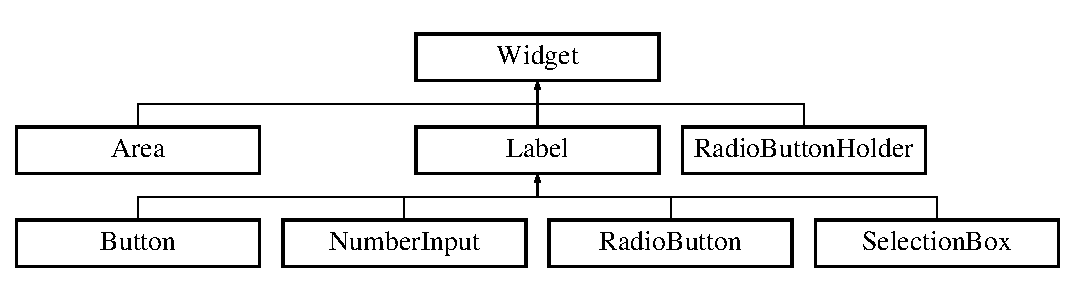
\includegraphics[height=3.000000cm]{class_widget}
\end{center}
\end{figure}
\subsection*{Publikus tagfüggvények}
\begin{DoxyCompactItemize}
\item 
\hyperlink{class_widget_a5a76a8d2fbb399fe02eb89782d1c3e99}{Widget} (int x, int y, int x\+Size, int y\+Size)
\item 
virtual void \hyperlink{class_widget_ac4c2063cd671468ad05d84cfe963c032}{Draw} ()=0
\item 
virtual void \hyperlink{class_widget_abf512e4606c7a5d44245a9b0246634a0}{Handle} (\hyperlink{structgenv_1_1event}{genv\+::event} ev)=0
\item 
virtual bool \hyperlink{class_widget_a7a18323ef481add82e5edba5c0c6ec06}{Is\+In\+Line} (int x, int y)=0
\item 
void \hyperlink{class_widget_ac614472479dfd7c3f54c3d1445647403}{Set\+Border\+Thickness} (int thickness)
\item 
void \hyperlink{class_widget_a714f8e9b39be7e3627cb7031a1ccbfc1}{Set\+Background\+Colour} (int r, int g, int b)
\item 
void \hyperlink{class_widget_ae8018660228f34e126830e1d951e3e39}{Set\+Front\+Colour} (int r, int g, int b)
\item 
\mbox{\Hypertarget{class_widget_aa7003624e0cda852437dcd4d31fbbd74}\label{class_widget_aa7003624e0cda852437dcd4d31fbbd74}} 
void {\bfseries Set\+Enable} (bool value)
\item 
\mbox{\Hypertarget{class_widget_ab44aee83ce8ca060f0164f2cbca53c27}\label{class_widget_ab44aee83ce8ca060f0164f2cbca53c27}} 
void {\bfseries Set\+Visible} (bool value)
\end{DoxyCompactItemize}
\subsection*{Védett attribútumok}
\begin{DoxyCompactItemize}
\item 
int \hyperlink{class_widget_a77cb3fae6d2c4287b57feec515fd247d}{X}
\item 
int \hyperlink{class_widget_a7632723033e771a3b4ed3f699a25a9e3}{Y}
\item 
int \hyperlink{class_widget_a0cc8f9439ec1b0327ae5226289dfaa6f}{X\+Size}
\item 
int \hyperlink{class_widget_abe9fda79928940f9befc857bea306a8d}{Y\+Size}
\item 
\hyperlink{class_colour}{Colour} $\ast$ \hyperlink{class_widget_a2b6dae3f5b5881a10dfbda5cdf1a6c08}{bg\+Color}
\item 
\hyperlink{class_colour}{Colour} $\ast$ \hyperlink{class_widget_a1abd0659ba3986b0666a959aaa0fdc44}{front\+Color}
\item 
int \hyperlink{class_widget_a15883515db90a056b6f79e563cbfbdc4}{border\+Thickness}
\item 
bool \hyperlink{class_widget_a6f559eace419b3371fe263b1de932054}{Selected}
\item 
\mbox{\Hypertarget{class_widget_a28f496ba72bd65d028c06b118964b7aa}\label{class_widget_a28f496ba72bd65d028c06b118964b7aa}} 
bool {\bfseries Is\+Enabled}
\item 
\mbox{\Hypertarget{class_widget_a7f22aaa455c2e0814ecad3974bb3aa89}\label{class_widget_a7f22aaa455c2e0814ecad3974bb3aa89}} 
bool {\bfseries Is\+Visible}
\end{DoxyCompactItemize}


\subsection{Konstruktorok és destruktorok dokumentációja}
\mbox{\Hypertarget{class_widget_a5a76a8d2fbb399fe02eb89782d1c3e99}\label{class_widget_a5a76a8d2fbb399fe02eb89782d1c3e99}} 
\index{Widget@{Widget}!Widget@{Widget}}
\index{Widget@{Widget}!Widget@{Widget}}
\subsubsection{\texorpdfstring{Widget()}{Widget()}}
{\footnotesize\ttfamily Widget\+::\+Widget (\begin{DoxyParamCaption}\item[{int}]{x,  }\item[{int}]{y,  }\item[{int}]{x\+Size,  }\item[{int}]{y\+Size }\end{DoxyParamCaption})}

Egy �j widgetet hoz l�tre. 
\begin{DoxyParams}{Paraméterek}
{\em x} & A widget X poz�ci�ja \\
\hline
{\em y} & A widget Y poz�ci�ja \\
\hline
{\em x\+Size} & A widget hossza \\
\hline
{\em y\+Size} & A widget magass�ga \\
\hline
\end{DoxyParams}


\subsection{Tagfüggvények dokumentációja}
\mbox{\Hypertarget{class_widget_ac4c2063cd671468ad05d84cfe963c032}\label{class_widget_ac4c2063cd671468ad05d84cfe963c032}} 
\index{Widget@{Widget}!Draw@{Draw}}
\index{Draw@{Draw}!Widget@{Widget}}
\subsubsection{\texorpdfstring{Draw()}{Draw()}}
{\footnotesize\ttfamily virtual void Widget\+::\+Draw (\begin{DoxyParamCaption}{ }\end{DoxyParamCaption})\hspace{0.3cm}{\ttfamily [pure virtual]}}

Ez felel a widget kirajzol�s��rt 

Megvalósítják a következők\+: \hyperlink{class_area_ac90399336ed7754946e274e443ed98ff}{Area}, \hyperlink{class_radio_button_holder_a70d6ba1724bdb68afe351d0474cbd767}{Radio\+Button\+Holder}, \hyperlink{class_radio_button_a296e30588da8a4767164c2dfc5d25a71}{Radio\+Button}, \hyperlink{class_label_a184df028b3aa8c7f8dec8ecb90533319}{Label}, \hyperlink{class_number_input_ab65631421ec222bb929f74d1782b5c8b}{Number\+Input}, \hyperlink{class_selection_box_a1c0b7b6c851180450964a4df0c7c15e8}{Selection\+Box} és \hyperlink{class_button_a6aaa2b781c933a296f41a8eca890eb1f}{Button}.

\mbox{\Hypertarget{class_widget_abf512e4606c7a5d44245a9b0246634a0}\label{class_widget_abf512e4606c7a5d44245a9b0246634a0}} 
\index{Widget@{Widget}!Handle@{Handle}}
\index{Handle@{Handle}!Widget@{Widget}}
\subsubsection{\texorpdfstring{Handle()}{Handle()}}
{\footnotesize\ttfamily virtual void Widget\+::\+Handle (\begin{DoxyParamCaption}\item[{\hyperlink{structgenv_1_1event}{genv\+::event}}]{ev }\end{DoxyParamCaption})\hspace{0.3cm}{\ttfamily [pure virtual]}}

Ez a f�ggv�ny kezeli az eventeket 
\begin{DoxyParams}{Paraméterek}
{\em ev} & Az aktu�lis event objektum \\
\hline
\end{DoxyParams}


Megvalósítják a következők\+: \hyperlink{class_area_a8917c7e4715659ae5021d2c9e40127f4}{Area}, \hyperlink{class_radio_button_holder_a7b4ed9e75eef252ad20c3cbcb8547981}{Radio\+Button\+Holder}, \hyperlink{class_radio_button_a9287d026f57bdfedd878269ec4648135}{Radio\+Button}, \hyperlink{class_button_a72dc68b7a78edfebe904bf489d6e03fb}{Button}, \hyperlink{class_label_a5cf04da7def075453b5c0fda93a1b575}{Label}, \hyperlink{class_number_input_a08a2de51093fe35c3c7b9998e88924a9}{Number\+Input} és \hyperlink{class_selection_box_a4762480ce86018d74c0cfa271c9cce11}{Selection\+Box}.

\mbox{\Hypertarget{class_widget_a7a18323ef481add82e5edba5c0c6ec06}\label{class_widget_a7a18323ef481add82e5edba5c0c6ec06}} 
\index{Widget@{Widget}!Is\+In\+Line@{Is\+In\+Line}}
\index{Is\+In\+Line@{Is\+In\+Line}!Widget@{Widget}}
\subsubsection{\texorpdfstring{Is\+In\+Line()}{IsInLine()}}
{\footnotesize\ttfamily virtual bool Widget\+::\+Is\+In\+Line (\begin{DoxyParamCaption}\item[{int}]{x,  }\item[{int}]{y }\end{DoxyParamCaption})\hspace{0.3cm}{\ttfamily [pure virtual]}}

Megadja, hogy az eg�r a saj�t keretein bel�l van-\/e 
\begin{DoxyParams}{Paraméterek}
{\em x} & Az eg�r X poz�ci�ja \\
\hline
{\em y} & Az eg�r Y poz�ci�ja \\
\hline
\end{DoxyParams}


Megvalósítják a következők\+: \hyperlink{class_area_a9d309a54dbc62cd8edd8bc976644090c}{Area}, \hyperlink{class_radio_button_holder_aa6d6fe7d9eb9ce9c2628f432ef129e01}{Radio\+Button\+Holder}, \hyperlink{class_radio_button_a94ab27ee37cdd639a185cb746ad7b32f}{Radio\+Button}, \hyperlink{class_button_a61832186fb0cf58c4c1c6fbbe572b61c}{Button}, \hyperlink{class_label_a918ebb45dbaa5484643355cf5ab4be47}{Label}, \hyperlink{class_number_input_af364cc666a41dfa189e024464e4bc317}{Number\+Input} és \hyperlink{class_selection_box_a0378e1ec035f90dd04efac5d6a2c7132}{Selection\+Box}.

\mbox{\Hypertarget{class_widget_a714f8e9b39be7e3627cb7031a1ccbfc1}\label{class_widget_a714f8e9b39be7e3627cb7031a1ccbfc1}} 
\index{Widget@{Widget}!Set\+Background\+Colour@{Set\+Background\+Colour}}
\index{Set\+Background\+Colour@{Set\+Background\+Colour}!Widget@{Widget}}
\subsubsection{\texorpdfstring{Set\+Background\+Colour()}{SetBackgroundColour()}}
{\footnotesize\ttfamily void Widget\+::\+Set\+Background\+Colour (\begin{DoxyParamCaption}\item[{int}]{r,  }\item[{int}]{g,  }\item[{int}]{b }\end{DoxyParamCaption})}

�t�l�tja a widget h�tt�rsz�n�t 
\begin{DoxyParams}{Paraméterek}
{\em r} & Az �j piros �rt�k \\
\hline
{\em g} & Az �j z�ld �rt�k \\
\hline
{\em b} & Az �j k�k �rt�k \\
\hline
\end{DoxyParams}
\mbox{\Hypertarget{class_widget_ac614472479dfd7c3f54c3d1445647403}\label{class_widget_ac614472479dfd7c3f54c3d1445647403}} 
\index{Widget@{Widget}!Set\+Border\+Thickness@{Set\+Border\+Thickness}}
\index{Set\+Border\+Thickness@{Set\+Border\+Thickness}!Widget@{Widget}}
\subsubsection{\texorpdfstring{Set\+Border\+Thickness()}{SetBorderThickness()}}
{\footnotesize\ttfamily void Widget\+::\+Set\+Border\+Thickness (\begin{DoxyParamCaption}\item[{int}]{thickness }\end{DoxyParamCaption})}

�t�l�tja a marg� vastags�g�t 
\begin{DoxyParams}{Paraméterek}
{\em thickness} & Az �j vastags�g \\
\hline
\end{DoxyParams}
\mbox{\Hypertarget{class_widget_ae8018660228f34e126830e1d951e3e39}\label{class_widget_ae8018660228f34e126830e1d951e3e39}} 
\index{Widget@{Widget}!Set\+Front\+Colour@{Set\+Front\+Colour}}
\index{Set\+Front\+Colour@{Set\+Front\+Colour}!Widget@{Widget}}
\subsubsection{\texorpdfstring{Set\+Front\+Colour()}{SetFrontColour()}}
{\footnotesize\ttfamily void Widget\+::\+Set\+Front\+Colour (\begin{DoxyParamCaption}\item[{int}]{r,  }\item[{int}]{g,  }\item[{int}]{b }\end{DoxyParamCaption})}

�t�l�tja a widget el�t�r sz�n�t 
\begin{DoxyParams}{Paraméterek}
{\em r} & Az �j piros �rt�k \\
\hline
{\em g} & Az �j z�ld �rt�k \\
\hline
{\em b} & Az �j k�k �rt�k \\
\hline
\end{DoxyParams}


\subsection{Adattagok dokumentációja}
\mbox{\Hypertarget{class_widget_a2b6dae3f5b5881a10dfbda5cdf1a6c08}\label{class_widget_a2b6dae3f5b5881a10dfbda5cdf1a6c08}} 
\index{Widget@{Widget}!bg\+Color@{bg\+Color}}
\index{bg\+Color@{bg\+Color}!Widget@{Widget}}
\subsubsection{\texorpdfstring{bg\+Color}{bgColor}}
{\footnotesize\ttfamily \hyperlink{class_colour}{Colour}$\ast$ Widget\+::bg\+Color\hspace{0.3cm}{\ttfamily [protected]}}

A h�tt�r sz�ne \mbox{\Hypertarget{class_widget_a15883515db90a056b6f79e563cbfbdc4}\label{class_widget_a15883515db90a056b6f79e563cbfbdc4}} 
\index{Widget@{Widget}!border\+Thickness@{border\+Thickness}}
\index{border\+Thickness@{border\+Thickness}!Widget@{Widget}}
\subsubsection{\texorpdfstring{border\+Thickness}{borderThickness}}
{\footnotesize\ttfamily int Widget\+::border\+Thickness\hspace{0.3cm}{\ttfamily [protected]}}

A marg� vastags�ga \mbox{\Hypertarget{class_widget_a1abd0659ba3986b0666a959aaa0fdc44}\label{class_widget_a1abd0659ba3986b0666a959aaa0fdc44}} 
\index{Widget@{Widget}!front\+Color@{front\+Color}}
\index{front\+Color@{front\+Color}!Widget@{Widget}}
\subsubsection{\texorpdfstring{front\+Color}{frontColor}}
{\footnotesize\ttfamily \hyperlink{class_colour}{Colour}$\ast$ Widget\+::front\+Color\hspace{0.3cm}{\ttfamily [protected]}}

Az el�t�r sz�ne \mbox{\Hypertarget{class_widget_a6f559eace419b3371fe263b1de932054}\label{class_widget_a6f559eace419b3371fe263b1de932054}} 
\index{Widget@{Widget}!Selected@{Selected}}
\index{Selected@{Selected}!Widget@{Widget}}
\subsubsection{\texorpdfstring{Selected}{Selected}}
{\footnotesize\ttfamily bool Widget\+::\+Selected\hspace{0.3cm}{\ttfamily [protected]}}

Ki van-\/e v�lasztva a widget \mbox{\Hypertarget{class_widget_a77cb3fae6d2c4287b57feec515fd247d}\label{class_widget_a77cb3fae6d2c4287b57feec515fd247d}} 
\index{Widget@{Widget}!X@{X}}
\index{X@{X}!Widget@{Widget}}
\subsubsection{\texorpdfstring{X}{X}}
{\footnotesize\ttfamily int Widget\+::X\hspace{0.3cm}{\ttfamily [protected]}}

A widget X koordin�t�ja \mbox{\Hypertarget{class_widget_a0cc8f9439ec1b0327ae5226289dfaa6f}\label{class_widget_a0cc8f9439ec1b0327ae5226289dfaa6f}} 
\index{Widget@{Widget}!X\+Size@{X\+Size}}
\index{X\+Size@{X\+Size}!Widget@{Widget}}
\subsubsection{\texorpdfstring{X\+Size}{XSize}}
{\footnotesize\ttfamily int Widget\+::\+X\+Size\hspace{0.3cm}{\ttfamily [protected]}}

A widget sz�less�ge \mbox{\Hypertarget{class_widget_a7632723033e771a3b4ed3f699a25a9e3}\label{class_widget_a7632723033e771a3b4ed3f699a25a9e3}} 
\index{Widget@{Widget}!Y@{Y}}
\index{Y@{Y}!Widget@{Widget}}
\subsubsection{\texorpdfstring{Y}{Y}}
{\footnotesize\ttfamily int Widget\+::Y\hspace{0.3cm}{\ttfamily [protected]}}

A widget Y koordin�t�ja \mbox{\Hypertarget{class_widget_abe9fda79928940f9befc857bea306a8d}\label{class_widget_abe9fda79928940f9befc857bea306a8d}} 
\index{Widget@{Widget}!Y\+Size@{Y\+Size}}
\index{Y\+Size@{Y\+Size}!Widget@{Widget}}
\subsubsection{\texorpdfstring{Y\+Size}{YSize}}
{\footnotesize\ttfamily int Widget\+::\+Y\+Size\hspace{0.3cm}{\ttfamily [protected]}}

A widget magass�ga 

Ez a dokumentáció az osztályról a következő fájlok alapján készült\+:\begin{DoxyCompactItemize}
\item 
Widget.\+h\item 
Widget.\+cpp\end{DoxyCompactItemize}

%--- End generated contents ---

% Index
\backmatter
\newpage
\phantomsection
\clearemptydoublepage
\addcontentsline{toc}{chapter}{Tárgymutató}
\printindex

\end{document}
